% Options for packages loaded elsewhere
\PassOptionsToPackage{unicode}{hyperref}
\PassOptionsToPackage{hyphens}{url}
%
\documentclass[
  12pt,
]{scrbook}
\usepackage[]{libertine}
\usepackage{amssymb,amsmath}
\usepackage{ifxetex,ifluatex}
\ifnum 0\ifxetex 1\fi\ifluatex 1\fi=0 % if pdftex
  \usepackage[T1]{fontenc}
  \usepackage[utf8]{inputenc}
  \usepackage{textcomp} % provide euro and other symbols
\else % if luatex or xetex
  \usepackage{unicode-math}
  \defaultfontfeatures{Scale=MatchLowercase}
  \defaultfontfeatures[\rmfamily]{Ligatures=TeX,Scale=1}
\fi
% Use upquote if available, for straight quotes in verbatim environments
\IfFileExists{upquote.sty}{\usepackage{upquote}}{}
\IfFileExists{microtype.sty}{% use microtype if available
  \usepackage[]{microtype}
  \UseMicrotypeSet[protrusion]{basicmath} % disable protrusion for tt fonts
}{}
\usepackage{xcolor}
\IfFileExists{xurl.sty}{\usepackage{xurl}}{} % add URL line breaks if available
\IfFileExists{bookmark.sty}{\usepackage{bookmark}}{\usepackage{hyperref}}
\hypersetup{
  pdftitle={A Guide to the Social Management of New Technology},
  hidelinks,
  pdfcreator={LaTeX via pandoc}}
\urlstyle{same} % disable monospaced font for URLs
\usepackage{longtable,booktabs}
% Correct order of tables after \paragraph or \subparagraph
\usepackage{etoolbox}
\makeatletter
\patchcmd\longtable{\par}{\if@noskipsec\mbox{}\fi\par}{}{}
\makeatother
% Allow footnotes in longtable head/foot
\IfFileExists{footnotehyper.sty}{\usepackage{footnotehyper}}{\usepackage{footnote}}
\makesavenoteenv{longtable}
\usepackage{graphicx}
\makeatletter
\def\maxwidth{\ifdim\Gin@nat@width>\linewidth\linewidth\else\Gin@nat@width\fi}
\def\maxheight{\ifdim\Gin@nat@height>\textheight\textheight\else\Gin@nat@height\fi}
\makeatother
% Scale images if necessary, so that they will not overflow the page
% margins by default, and it is still possible to overwrite the defaults
% using explicit options in \includegraphics[width, height, ...]{}
\setkeys{Gin}{width=\maxwidth,height=\maxheight,keepaspectratio}
% Set default figure placement to htbp
\makeatletter
\def\fps@figure{htbp}
\makeatother
\setlength{\emergencystretch}{3em} % prevent overfull lines
\providecommand{\tightlist}{%
  \setlength{\itemsep}{0pt}\setlength{\parskip}{0pt}}
\setcounter{secnumdepth}{5}
% Authors for each chapter
\newenvironment{chap-auth}
{\vspace{1cm}\begin{center}\begin{flushright}\sffamily\noindent}
  {\end{flushright}\end{center}\vspace{1cm}}

% Fix identations
\usepackage{indentfirst}

% Fix headings
\usepackage{scrlayer-scrpage}

% Fix windows and orphans...
\widowpenalty=10000
\clubpenalty=10000
\newlength{\cslhangindent}
\setlength{\cslhangindent}{1.5em}
\newenvironment{cslreferences}%
  {}%
  {\par}

\title{A Guide to the Social Management of New Technology}
\author{Joel Lööw \& Jan Johansson\\
~\\
\emph{Editors}}
\date{2020-06-11}

\begin{document}
\maketitle

{
\setcounter{tocdepth}{0}
\tableofcontents
}
\hypertarget{preface}{%
\chapter*{Preface}\label{preface}}
\addcontentsline{toc}{chapter}{Preface}

This book is a product of the \href{http://simsmining.eu}{SIMS (Sustainable Intelligent Mining
Systems)} project, which is funded by the European
Union. The vision of SIMS is to create a long-lasting impact on how we
test and demonstrate new technology and solutions for the mining
industry. With a selected consortium ranging from mining companies,
equipment and system suppliers to top-class universities, the SIMS
project will boost development and innovation through joint activities
aiming at creating~sustainable intelligent mining systems.

Our role in the project is to be involved in creating attractive
workplaces by deeply interacting with other work project partners and
influencing their designs. Our role also includes ensuring that gender
aspects are considered in the various parts of the projects. We also
have an important role in the social acceptance of the new technology.

\hypertarget{about-the-authors}{%
\section*{About the authors}\label{about-the-authors}}
\addcontentsline{toc}{section}{About the authors}

\begin{description}
\tightlist
\item[Jan Johansson]
is project manager for the SIMS subproject Attractive Workplaces, is a
professor of Human Work Science at Luleå University of Technology (LTU)
in Sweden.
\item[Joel Lööw]
is a PhD student in Human Work Science at LTU. Together with Jan
Johansson, he edited this book.
\item[Lena Abrahamson]
is a chair professor in Human Work Science at LTU.
\item[Eira Andersson]
is a senior lecturer in Human Work Science at LTU.
\item[Lisa Öman Ekervhén]
is a senior lecturer in Engineering Psychology at LTU.
\item[Camilla Grane]
is a senior lecturer in Engineering Psychology at LTU.
\item[Bo Johansson]
is a associated professor in Human Work Science at LTU.
\item[Magnus Nygren]
is a senior lecturer in Human Work Science at LTU.
\item[Lisa Ringblom]
is a post doc researcher at the Centre for Work Life and Evaluation
Studies at Malmö University.
\item[Eugenia Segerstedt]
is a PhD student in Human Work Science at LTU.
\item[Erik Sundström]
is a PhD student in Human Work Science at LTU.
\end{description}

\hypertarget{introduction}{%
\chapter*{Introduction}\label{introduction}}
\addcontentsline{toc}{chapter}{Introduction}

\markboth{A Guide to the Social Management of New Technology}{Introduction}
\pagestyle{myheadings}

\begin{chap-auth}
Joel Lööw and Jan Johansson (Editors)
\end{chap-auth}

Today's mining industry is facing major technical changes. Earlier incremental development will most certainly be replaced by more radical changes based on digitization and the Internet of Things. These changes must be managed in a socially sustainable way so that we do not create greater problems than those we are solving. We must design tomorrow's mining so that it can gain social acceptance. Tomorrow's mining companies must be able to offer safe and attractive workplaces that can attract young people to the industry. From a longer perspective, offering such workplaces can lead to the recognition of the mining industry as an ethical, ecological and diverse industry that can offer challenging jobs and attractive workplaces. The purpose of this book is to provide advice and simple guidance for how to develop and introduce something we call social management of new technology. We hope that this summary of our experiences from the SIMS project can be useful to you and wish you pleasant reading.

The book is formatted similar to a Swedish smorgasbord. In other words, each chapter can be read independently. Consequently, there may be some repetition. Most chapters end with several summarizing practical advice points.

The book consists of 22 chapters. All the chapters are available for
computers, tablets and mobile phones on \url{https://jloow.github.io/wp8-book/}.

In chapter 1, The future of metal mining, we discuss the challenges facing today's metal mining industry. We make 15 predictions about the future that should be seen as a contextual background to the discussions in the following chapters.

In chapter 2, A vision of ``The New Attractive Mine'', we have tried to create a vision of a future mine, considering the working environment and attractiveness all the way from the mine planning stage.

In chapter 3, What characterizes an attractive mining workplace?, we have used a general model that describes 22 dimensions of what characterizes an attractive workplace and applied it to the mining industry.

In chapter 4, Attracting young people to the mining industry, we have summarized our findings in six recommendations for creating attractive workplaces and increasing the visibility of the good parts of mining work.

In chapter 5, Attractive workplaces do not fit all, we try to give nuance to the concept of attractive workplaces by showing its complexity. Throughout the book, we argue for a participative approach that is based on the wishes of the employees, but occasionally you meet opposing wishes and have to take a position based on other criteria.

In chapter 6, Meeting social challenges in established mining communities, we broaden the frame of reference and discuss the mining industry's responsibility to operate in a socially sustainable society.

In chapter 7, Risk analysis and prevention, we focus on the safety aspects and present practical models for risk assessment. We underline the role of the mine planners; they must find solutions that promote both high productivity and good economy and also safety and a healthy work environment.

In chapter 8, Safe and attractive workplaces for contractor personnel, we address the fact that workplace accidents are a problem in relation to outsourcing and contracting. We indicate several points that can be taken into consideration when aiming to increase safety in these types of work setting.

In chapter 9, Understanding, and improving, safety culture, we discuss improved safety culture as a long term and sustainable safety strategy. We suggest measures that mining companies can take when seeking to develop their safety culture.

In chapter 10, Gender and gender equality in mining, we present a brief theoretical background on why gender is an important issue for the mining industry. The chapter ends with general advice.

In chapter 11, Can technology improve gender equality in mining?, the myth that new technology will automatically open the mines for women is highlighted. More systematic work is required to correct the uneven gender balance.

In chapter 12, Working for gender equality in organizations -- a model, we present a practical model for how to work with gender equality, work that is necessary if mining is to be considered a modern industry.

In chapter 13, Lean mining -- lean production and the mining industry, we discuss the concept of lean production and how it can be adapted to the mining industry and form the basis of what we call lean mining.

In chapter 14, Industry 4.0 in a mining context, we explore the consequences that digitalization and Industry 4.0 can have on future mining work. A vast majority of mining work will be affected by these developments, but miners will not disappear; rather, they will be different in the future.

In chapter 15, Mining 4.0 -- Utopia or Dystopia, we summarize our experiences with two extremes, a negative dystopian development and a positive utopian development. The chapter concludes with six recommendations on how to start shaping the future of Mining 4.0 on human terms.

In chapter 16, Acceptance of new technology -- the most prominent theories, we give an overview of the most prominent theories that are important for understanding which factors affect the acceptance of new technologies.

In chapter 17, Positioning technology -- safety vs privacy concerns, we discuss the positive effects of positioning technology from a safety perspective and set them against privacy concerns. Factors that need to be considered to enhance privacy and reduce the perception of misuse are discussed.

In chapter 18, Investing in new technology: guidelines for how to do it right or to understand what went wrong, we provide guidelines, or statements to consider, when investing in new technology. These questions are meant to aid the organization in the process towards technology and in making that process effective, efficient and accepted from a user perspective.

In chapter 19, Adapting the technology to the miners' human factors, we present a theory for human-centred design, which is a theory for designing equipment, workplaces, tasks and organizations on human terms.

In chapter 20, Iterative design of mining workplaces, we describe a circular method for mining planning that is more dynamic than today's linear planning. Furthermore, an iterative process offers more opportunities to create attractive workplaces for both new and existing employees by involving them more in the design process.

In chapter 21, More research is needed, we present a research agenda that focusses on attracting and keeping skilled personnel in a future high-tech mining industry.

In chapter 22, Checklist for safe and attractive mining workplaces, we summarize our results in a practical checklist. There are many aspects, issues and questions that must be considered and addressed to achieve safe and attractive mining workplaces. This checklist aims to help highlight potential areas of improvement in a mining workplace that could make it a safer and more attractive workplace, without presenting in-depth solutions that may limit the decision-making process.

\clearpage
\pagestyle{headings}
\automark[chapter]{chapter}
\lehead{A Guide to the Social Management of New Technology}

\hypertarget{the-future-of-metal-mining}{%
\chapter{The future of metal mining}\label{the-future-of-metal-mining}}

\begin{chap-auth}
Jan Johansson, Lena Abrahamsson and Bo Johansson
\end{chap-auth}

In this chapter, we will discuss the challenges facing today's metal mining industry. Our statements about the future should be seen as a contextual background to the discussions presented in the following chapters

The world's metal mining industry is rapidly changing and faces several challenges that must be addressed with a sociotechnical approach that covers the whole mining and minerals value adding chain, including environmental issues. We have tried to capture this uncertain future in fifteen predictions presented below:

\begin{enumerate}
\def\labelenumi{\arabic{enumi}.}
\item
  Future mining will be shaped in a context where it is necessary to produce at costs that are determined in \emph{international competition}. The prices of metals and minerals are set by the market, but in the long term, there is little doubt that the demand is increasing. Large nations such as China, India, Indonesia, Brazil and the whole of Africa will require a larger share of consumption, which is leading to the opening of new mines. The difference between these countries' annual ``per capita'' consumption and Western Europe can be greater than 10 times.
\item
  Production conditions will be characterized by the fact that nearby and easily accessible ores will be mined first. \emph{New ores will also become more distant or found in the depths}. Large ore reserves are located under the sea, and there is little doubt that the mining and offshore companies will develop new technology to extract these reserves. In both cases, production costs will increase.
\item
  Mining depths increase, and that increase brings new stability problems. The role of rock mechanics in the design of layouts, cutting sequences, strata stabilization, and roof bolting, etc., must be a central issue for the future. \emph{Full face drilling and cutting} should be interesting from a safety perspective, both directly in safer drifting operations and because it can create more-stable galleries due to reduced or no blasting damages. Cutting should also be useful for selective mining of high-quality ore in narrow ore bodies. Production drilling and blasting for \emph{controlled fragmentation} are two very crucial operations in the ore mining cycle. Improvements in these operations open up many possibilities for \emph{automation}.
\item
  \emph{Environmental requirements} affect both energy consumption and management of ore tailings. The discussion of energy consumption is largely linked to global warming and carbon emissions. Today, not all nations have joined the Paris Climate Agreement, but in the long term, some form of coordination surely will be established. The cost of emission allowances will be a significant factor to consider.
\item
  The mining industry is an \emph{energy-intensive industry}, with high CO\textsubscript{2} emission. Improvement of energy efficiency will increase economic profitability and reduce environmental impact. There are many components that affect total energy consumption; one often discussed is underground pre-concentration (\emph{in situ}). This approach directly affects the energy-consuming hoisting and milling. The use of fossil diesel fuel is extensive and causes environmental burdens. A transition to electric power and battery operation is in progress.
\item
  The discussion of \emph{waste management} is about leaving as few footprints in nature as possible. We must not leave toxic substances that leak out into nature, and the landscape should be restored as much as possible. One solution discussed is \emph{in situ mining}, where as much as possible of the production and processing will take place underground. Such technology is however not without environmental risks and risks for health and safety. Pollution of mine water is the single most important environmental issue for the mining sector and consequently also affects mine water treatment. Regarding water in general, it is a question of \emph{closing the loop}s and re-using the process water as much as possible.
\item
  The environmental debate also includes a discussion on the mining industry's \emph{social responsibility} for the welfare of the local community. In addition to preserving the environment, they are supposed to build a strong technical and social infrastructure that ensures the survival of society after mining has ceased.
\item
  Health and safety at work must have top priority. Mechanization, remote control and automation are efficient preventive safety measures. They are also appropriate for reducing workload to avoid musculoskeletal injuries and allow for recovery periods. New technology makes it possible to both warn of dangerous working conditions and monitor employees' health conditions in real time. Improved safety is also a matter of a developed safety climate in the form of relevant education, rules and effective leadership, with safety prioritized in the day-to-day workplace.
\item
  Many problems in the work environment in present mines (and in other industries) can be traced back to insufficient initial physical planning and design. Since mining is characterized by huge investments and long-term operations, it is very important to have a well-designed physical production system. The physical layout also influences and limits the organizational aspects. If initial mistakes are made, personnel will have to bear the negative consequences for many years to come. The initial design phases of every major development project are therefore critical for establishing a safe and attractive physical and psychosocial work environment in a mine.
\item
  \emph{Industry 4.0} is based on implementations of the Internet of Things, 5G and big data, where the entire production process is included in internet-based networks that transform the mines into smart mines. We will soon see the outlines for Mining 4.0, where miners equipped with minicameras can, for everyday and emergency situations, provide their colleagues and senior management with information that is difficult to convey verbally.
\item
  \emph{The extended business} and \emph{open collaboration} are two concepts where Virtual Reality (VR) technology can be used to link production functions such as planning, mining, maintenance, logistics, purchasing and for the coordination of external contractors, suppliers, and customers, etc., all connected to a production flow, a value adding chain, where all share the same goal and everyone sees the same whole. Common visualization of problems and opportunities in the system allows for all to optimize the whole chain rather than suboptimizing parts.
\item
  N\emph{ew professional roles} with a higher proportion of remote control from production centres and \emph{collaborative visualization rooms}, perhaps located in nearby communities or further away (other continents), where the operators have monitoring and coordinating activities across the value chain. Their jobs will change character towards service work, and the new tasks require different kinds of skills. In addition to dealing with advanced information technology, the miners have to interact with different specialist teams located all over the world.
\item
  New technology creates a new type of work -- new in terms of \emph{competencies and knowledge} and workload. There is an emerging, and in many aspects already evident, knowledge transformation from the old and obsolete physical and tacit knowledge and skills (for example, the ability to `read the rock') to something new that can be described as abstract knowledge. This transformation can challenge the identity of the miners and create resistance to change.
\item
  Future efficient mining operations will be dependent upon a highly competent and well-motivated work force, on all levels. The mining companies will have to recruit their personnel from a limited group of talented individuals with high demands and expectations with respect to future work. To cope with the future labour supply, the mining industry must change the image of mining work and increase the attractiveness of working in the sector, especially for young women and men.
\item
  The mines of the future will have smaller staffing, and it is also clear that they will meet a different kind of \emph{model for work organization} than they do today. Mining companies will gradually turn to a flat and \emph{lean organization} with multiskilled workers who can operate in several areas and functions within the company. There is also a discussion about a staffing system based on the \emph{fly-in/fly-out} method, which is more independent of a local community.
\end{enumerate}

There are of course other important areas of development, but those discussed above are expressed as the most important from a long-term strategic and sustainable view. A major conclusion is that the challenges and the changes are so large and numerous that comprehensive international cooperation is needed both within and outside the industry to succeed. Working separately would lead to a far too slow development, something that is undesirable for both the companies and the miners. Another conclusion is that a successful mining industry must work simultaneously with all the problems mentioned above. There is a need for a new and modern vision for the whole industry based on a sociotechnical approach that covers the whole mining and minerals value adding chain including environmental issues.

\hypertarget{a-vision-of-the-new-attractive-mine}{%
\chapter{A vision of ``The New Attractive Mine''}\label{a-vision-of-the-new-attractive-mine}}

\begin{chap-auth}
Jan Johansson and Bo Johansson
\end{chap-auth}

In this chapter, we have tried to create a vision of a future mine, considering the working environment and attractiveness all the way from the mine planning stage.

The new deep metal mine was a true planning and cooperation success and a huge leap in mining history. Several leading ``European mining companies'' had been inspired by the EU "Sustainable Intelligent Mining Systems" project, which is abbreviated as SIMS. This successful project had provided a conceptual system for automated and flexible mining, based on drill and blast technology for fragmentation of the actual ore. Continuous mining with road headers was still only used in development works where conventional drilling and blasting was abandoned. The zero entry mine was now almost realized, and the large ``European manufacturers of advanced mining equipment'' had contributed largely to the technological success, which had opened a new global market for them.

The new automated mining method made it possible to almost continuously produce desired ore qualities and quantities on customer demand. This ability was a large comparative advantage compared with the old traditional bulk production mines that still existed and struggled for survival. The new mining system dramatically reduced the prevailing and traditional use of expensive storing and stacking of mined ore. With the new approach to mining, an important first step towards true lean-mining was taken; gradually, one bottleneck after another was discovered and eliminated. Metal recovery was very high, and cut-off grades were reduced. It seemed as though traditional mining had been a real waste of resources.

Advanced investment analyses had clearly shown that there were great financial benefits with the new automated mining technology. The costs for underground development works were reduced by approximately 50\% compared with traditional mining methods, and labour costs were reduced by more than that. These cost reductions made it possible for the companies to make large investments in new technology and personnel competence and still be highly profitable. If profits for society and individuals were also included in the analysis, the total expected financial benefits where overwhelming. Follow-up of actual economical results showed even greater savings than expected.

An unusual feature of the new mine was that open pit mining was avoided, although the upper parts of the ore body were close to the surface. A green mining philosophy, ``\emph{In situ} mining'', was applied, and most of the mining activities were invisible for people passing the mine site. Most of the waste material was directly used for backfilling after recovering the metal content.

The mining companies had from the start of the project made use of a newly developed iterative planning methodology that reduced common initial design errors when they designed the new mine. Basic guidelines provided very useful demands for the mine designers. During the development work, there had for example never been any real ventilation problems, stability problems or water drainage problems. No severe accidents or incidents had occurred so far, and all mining activities were systematically risk assessed. The new mine had set a new world standard for results regarding health and safety results. Safety first was not only a simple slogan; it was a complex and applied reality. In fact, no major physical work or main activities were performed unless they had been computer simulated, evaluated and approved. This proactive means of addressing production and safety risks had proven its value time after time. The old description of mining work as ``dark, dirty and dangerous'' had definitively become out of date and irrelevant. Instead of being almost unpredictable and uncertain, mining had become highly predictable. Some of the old miners felt that the original charm of mining was somewhat lost when all worked according to plans, but no one truly wanted the old risky ways and days back.

One key to the success was the fact that the mine was already from the start designed for automation and sociotechnical principles, with a work organization based on production teams and broad professional skills among management and miners. One of the mine's most impressive features was the information and decision systems based on sensor technology and production analysis in real time. This system made it possible for the personnel to actively steer and control production instead of just passively reacting to deviations and alarms from an automated production process. This ability constituted a major difference and advantage compared with traditional control room work in, for example, regular processing plants. Impressive results regarding product quality and production availability and stability had been achieved due to this proactive philosophy. The philosophy also made the miners' work interesting and challenging.

The new remote-operations control centres (ROCs) were designed to promote cooperation and creative problem-solving in multiskilled teams. The working teams were mixed regarding age, experience, gender, and competence, etc. Diversity had replaced conformity and proved a good base for creating ``production scouts'', miners who were always ready and interested in improving the mining processes. Most of the team members were recruited from national and regional education programmes that were specifically developed with regards to the new demands that the mining sector had, basically that modern mining was intellectual analytical work for wise and reliable persons. New education programmes on all levels had been started and were recruiting well. Mining work had become attractive, not only because of the wages but also because it was very interesting work with good possibilities for personal and professional development in a safe and sound working environment.

Total progress had been astonishing, although they had only started to utilize parts of the potential that the new technology and organization offered. Investments in research and development work had paid off quickly, and management were convinced that innovative R\&D combined with a challenging vision had been and would continue to be the key factor for success.

\hypertarget{what-characterizes-an-attractive-mining-workplace}{%
\chapter{What characterizes an attractive mining workplace?}\label{what-characterizes-an-attractive-mining-workplace}}

\begin{chap-auth}
Erik Sundström
\end{chap-auth}

As mentioned in chapter 1, the mining industry has had difficulty with hiring people from younger generations and should therefore look for ways to improve the attractiveness of mining workplaces. However, it is not so easy to know what characterizes attractive mining work. We have chosen to use a general model that consists of 22 dimensions described by Åteg, Hedlund and Pontén (2004). In an effort to investigate whether and how these aspects of attractive work could be applied to mining workplaces, Lööw, Johansson, Andersson, \& Johansson (2019) examined the 22 dimensions and their relation to the mining industry. Below is a list describing each of the dimensions; the list includes descriptions of how they are best fulfilled and how mining workplaces are affected by and can affect the attractiveness of the workplace.

\hypertarget{attractive-working-conditions}{%
\section*{Attractive working conditions}\label{attractive-working-conditions}}
\addcontentsline{toc}{section}{Attractive working conditions}

\begin{itemize}
\item
  \emph{Adequate equipment and tools:} Modern equipment capable of providing good results efficiently and safely should be provided. Equipment should be designed to accommodate people of different sizes and with different needs.

  \begin{itemize}
  \tightlist
  \item
    Equipment in the mining industry has a history of having trouble accommodating the people that use it. With new technologies comes opportunities to design attractive equipment that accommodates both new and existing employees' needs.
  \end{itemize}
\item
  \emph{Leadership:} There should exist proper trust, communication and cooperation between employees and management. Management should feel safe letting the operators have more control over the planning and execution of work tasks and with letting them partake in decision making. Employees should feel as though they can safely give suggestions and voice concerns, while also trusting that management will take their needs into account when making changes.
\item
  \emph{Location:} It is important that the workplace is located close to home, that there is proper transportation to work and that the surrounding society is developed.

  \begin{itemize}
  \item
    Mining companies cannot easily accommodate this aspect due to being bound by mineral deposits' locations. However, by providing adequate transportation and housing, and investing in local societies, they can mitigate the negative effects on attractiveness.
  \item
    While bringing in personnel through fly-in/fly-out methods is an alternative, European mines generally try to avoid relying on such methods.
  \end{itemize}
\item
  \emph{Loyalty:} Employees should be loyal to and be treated with loyalty from the company, their colleagues and across organizational boundaries by cooperating and making sacrifices for each other.

  \begin{itemize}
  \item
    \emph{Establishing trust is an important factor for promoting loyalty. Management must ensure that the employees can trust them to make decisions and changes that are designed with their needs in mind.}
  \item
    \emph{Another important factor is to provide transparency. Management should detail and explain how and why certain decisions are made, which in turn should help build trust.}
  \end{itemize}
\item
  \emph{Organization:} A successful company can be more attractive, in addition to having low turnover, being in a good economic situation and providing advancement possibilities and benefits. The size of the organization also affects its attractiveness; smaller companies tend to be more attractive.

  \begin{itemize}
  \tightlist
  \item
    In modern mining companies, there is a trend amongst organizations to adapt something called lean mining. It is meant to help rationalize and make their production and organizations more effective by implementing lean philosophies. It entails a focus on quality of infrastructure and safety, production uptime, flexible and multiskilled workers, and teamwork.
  \end{itemize}
\item
  \emph{Physical work environment:} Attractive locales should have nice appearances and furnishing, pollutant-free air, and low sound levels, and they should be clean.

  \begin{itemize}
  \item
    The move towards control-room work helps mitigate negative impacts by removing the operators from the potentially risky mining workplaces for much of the work.
  \item
    Proper ventilation, noise protection and tunnels clear from debris are vital for a good work environment in a mine, even with more remote-controlled work.
  \end{itemize}
\item
  \emph{Relations:} The employees need relations in the workplace that provide support and empathy, with good team spirit, camaraderie, cooperation, honesty and so on.

  \begin{itemize}
  \tightlist
  \item
    Future mining work provides good opportunities to develop good work relationships with your colleagues if team members work in the same control rooms.
  \end{itemize}
\item
  \emph{Social contact:} The workplace allows for social interactions with other people, such as customers or colleagues.

  \begin{itemize}
  \item
    With control room work, people can more easily speak with their colleagues face-to-face.
  \item
    As mining work may occasionally require working alone, proper equipment for communication should be provided to avoid isolating operators.
  \end{itemize}
\item
  \emph{Wage:} It is important that the wage provided is of a sufficient level that it allows for people to support themselves and that it gradually increases.

  \begin{itemize}
  \item
    Wages in mining workplaces are generally higher than average, which could contribute to attractiveness, should other factors be addressed.
  \item
    Wages should not be based on produced results, both to provide a stable wage and to promote healthier ways of working, because piece rate wages have been shown to increase the risk of workplace accidents occurring, as they lead to safety procedures being neglected to increase production rates.
  \end{itemize}
\item
  \emph{Working hours:} Reasonable working hours that are predetermined and configurable can make a workplace more attractive. The employees should always know when they start and get off work, while also being able to influence the scope and distribution over the week and plan vacations.

  \begin{itemize}
  \item
    Mining usually relies on around-the-clock working hours. Setting up offices in larger cities that remotely control machines in the mines far away would access a larger employee base, making it easier to find people willing to accommodate these working hours.
  \item
    Working in extended shifts of 10-12 hours is common in the mining industry, but longer shifts increase the risk for accidents to occur. Thus, it should be avoided in favour of more standard working hours of approximately 8 hours per shift.
  \end{itemize}
\end{itemize}

\hypertarget{attractive-work-content}{%
\section*{Attractive work content}\label{attractive-work-content}}
\addcontentsline{toc}{section}{Attractive work content}

\begin{itemize}
\item
  \emph{Familiarity:} The employee should know what to do and what to expect in the workplace. This goal requires proper training, access to work instructions and an incentive to utilize that information.

  \begin{itemize}
  \tightlist
  \item
    With the implementation of 5G in mines and a digitalization of work, it will become easier to communicate with others and access work instructions whenever needed, even when below ground.
  \end{itemize}
\end{itemize}

\begin{itemize}
\item
  \emph{Freedom of action:} The employees should be able to organize and control their own and others' work, for instance by influencing the planning and execution of work tasks.

  \begin{itemize}
  \item
    Working from control rooms and with digitalized systems could give more opportunities for controlling one's work. For example, operators could more easily swap between and choose which machines in what parts of the mine to operate.
  \item
    Freedom of action could also be provided by placing the lowest planning level at the workgroup level. Management would no longer need to create individual plans and schedules for each employee. Instead, the workgroups would be provided with goals and missions after which they could plan their work accordingly, thus giving the workgroups more control over their work.
  \end{itemize}
\item
  \emph{Physical activity:} The workplace should allow and include healthy physical activity and movement to help prevent employees from suffering static work-related injuries or health problems.

  \begin{itemize}
  \tightlist
  \item
    After the automation, mechanization and digitalization of the mining industry, there will still be physical activities available, for example through maintenance work. Having the operators alternate between these tasks and control room work would help vary the otherwise very static workplace.
  \end{itemize}
\item
  \emph{Practical work:} The workplace should include practical and creative work tasks with handheld machines or tools to break from working only with computers or control systems.

  \begin{itemize}
  \tightlist
  \item
    This aspect can also benefit from including maintenance work to vary the control room work. Furthermore, since the new technologies will likely require adapting into the already complex mining systems of today, there will be opportunities for more creative work through retrofitting.
  \end{itemize}
\item
  \emph{Mental work:} Work tasks or problem solving should include cognitive work in addition to physical work and should be performed cooperatively with colleagues and management. This goal should include workplace learning, development and training.

  \begin{itemize}
  \item
    Control room work in mining industries offers many opportunities for mental work and brings groups of operators together in the same workplace.
  \item
    A more digitalized organization would enable easier communication and cooperation between groups that would otherwise rarely meet.
  \end{itemize}
\item
  \emph{Variation:} Throughout the day, employees should be provided opportunities for job rotation, development of work tasks and flexibility in ways to perform the tasks to prevent potential ergonomic and mental loads from working repeatedly with the same tasks.

  \begin{itemize}
  \item
    While remote-controlled mining workplaces may allow for rotating between work tasks, there might be less variation between tasks, as they would all be controlled through computer systems in control rooms. Including maintenance work tasks could help introduce more variation in work content and working environments, making the job less monotonous.
  \item
    Variation between work tasks requires that the employees are trained in how to handle the different tasks.
  \end{itemize}
\item
  \emph{Work pace:} The work pace should include both intensive and calm periods to engage people while also providing opportunities for rest and reflection.

  \begin{itemize}
  \tightlist
  \item
    Since the work pace in mining is continuous around the clock, there are few calm periods outside of assigned breaks. Introducing autonomous or semi-autonomous machines to the mining workplace would allow for more opportunities for calmer periods during the work. As an example, mining vehicles could autonomously drive to their destination, allowing the operator a short break from active work. The operator could then take control during more complicated or critical tasks once the vehicle has arrived.
  \end{itemize}
\end{itemize}

\hypertarget{work-satisfaction}{%
\section*{Work satisfaction}\label{work-satisfaction}}
\addcontentsline{toc}{section}{Work satisfaction}

\begin{itemize}
\item
  \emph{A demand for the person:} Workplaces where the employees feel as though they are needed and that they perform important work are generally considered more attractive.

  \begin{itemize}
  \item
    As the mining industry needs more skilful people and people from younger generations, those people may become more interested in the job if that demand can be communicated to them.

    \begin{itemize}
    \tightlist
    \item
      Potential ways to communicate the demand could include having a presence in mining-related education to show students that they are in demand.
    \end{itemize}
  \item
    Existing employees could feel more appreciated if the importance of their knowledge and skillsets is made more apparent to them.
  \end{itemize}
\item
  \emph{Recognition:} The employees should themselves feel that they have done a good job, in addition to being provided recognition for their work from management, colleagues or customers. Good performance should be rewarded according to the employee's subjective preference, perhaps through a monetary reward or through more time off.
\item
  \emph{Results:} The employees need to clearly understand what the results of their work are and how their work contributes to the workplace.

  \begin{itemize}
  \item
    The switch from operating the machines yourself to controlling them from a remote-control room could cause some disconnect from their work for the employees.
  \item
    Working from a control room with more digital systems provides a good opportunity to visualize and present the operators with an overview of the entire mine process.
  \end{itemize}
\item
  \emph{Status:} The workplace contributes to and strengthens an employee's sense of pride, success and professional identity. Companies must communicate to their employees the value of their work and their knowledge.

  \begin{itemize}
  \item
    The mining industry has had an image of heavy, tough and dirty but profitable work for a long time. The change towards more digital and remote work could impact that image and in turn impact people's perception of the industry.
  \item
    As many existing employees have established a sense of pride from working in the current mining industry, changing how mines are operated might negatively affect the attractiveness of the job for them.
  \item
    At the same time, moving towards the implementation of more-modern technologies could make the industry more attractive to younger generations of employees.
  \end{itemize}
\item
  \emph{Stimulation:} The workplace provides an opportunity for the employees to exert effort and use their skills in their work. The work being too difficult can be demoralizing for them, while it being too easy can lower the employees' motivation.

  \begin{itemize}
  \item
    The mining workplaces of today and of the future both provide opportunities for stimulating work; however, they may be stimulating in different ways. A current employee may find future mining workplaces to be unstimulating, while future employees may find the opposite.
  \item
    Regardless of what subjective views employees have of the work, they need to be provided with proper training and support if the work is difficult to them.
  \end{itemize}
\end{itemize}

While these dimensions cover many of the aspects that can affect the attractiveness of work, there is one important subject that remains largely unmentioned, namely, gender. Creating workplaces that are attractive for and accommodate both men and women is important if the mining industry wants to address the issue of hiring younger and skilful people. Otherwise, the mining industry runs the risk of driving away many potential applicants who otherwise could have been interested.

Although mining workplaces have the potential to fulfil the dimensions of attractiveness, it could still be difficult to accommodate each of these aspects simultaneously. However, this challenge does not mean that the workplace cannot be attractive if it only fulfils most or some aspects. What is important is that the parts of the workplace that negatively affect attractiveness are being compensated for through other positive aspects to ensure that the negative impact is lessened. For example, if heavy and ergonomically unhealthy tasks are unavoidable, supportive equipment and opportunities for rest in between can be used to lessen the negative impact. That way, an image of a safe and accessible workplace can better be conveyed and maintained.

\hypertarget{attracting-young-people-to-the-mining-industry}{%
\chapter{Attracting young people to the mining industry}\label{attracting-young-people-to-the-mining-industry}}

\begin{chap-auth}
Jan Johansson, Bo Johansson, Joel Lööw, Magnus Nygren and Lena
Abrahamsson
\end{chap-auth}

In most mines, the present workforce is ageing, and mining companies have difficulties recruiting young talented people. A precondition for being able to recruit the right workforce is that the mining industry can offer workplaces that attract the youths of tomorrow. To succeed, the mining companies need to know what in fact constitute attractive jobs and workplaces in mining and how they can change their own present operations to align with these requirements. These changes need to be based on current and relevant research on work attractiveness. However, labour supply is determined not only by the work itself and the working environment but also as much by the society and what it can offer its members. Several factors affect the attractiveness of society, such as social relations with family, friends and relatives, and opportunities regarding work and education, housing and leisure activities. These factors must also be considered when creating the mines of the future.

Unfortunately, there is no single accepted definition of what constitutes an attractive job, and current explanations and models differ. While pay and the possibilities of advancement are two general factors, answers have varied in, for example, different time periods and fields of research. It follows that what is attractive also differs between countries, since the general contexts and individuals differ.

A general model for attractive work is presented by Åteg et al.~(2004). In this model, three factors, covering 22 dimensions (see tbl.~\ref{tbl:table41}), interact and contribute to the attractiveness of work. For a detailed description of the various dimensions, see chapter 3. In comparison with previous, similar models, Åteg et al.~have added work satisfaction as a factor. This factor is especially important for keeping people at work, Åteg et al.~argue.

\hypertarget{tbl:table41}{}
\begin{longtable}[]{@{}lll@{}}
\caption{\label{tbl:table41}Work attractiveness}\tabularnewline
\toprule
\begin{minipage}[b]{0.37\columnwidth}\raggedright
Attractive working conditions\strut
\end{minipage} & \begin{minipage}[b]{0.30\columnwidth}\raggedright
Attractive work content\strut
\end{minipage} & \begin{minipage}[b]{0.24\columnwidth}\raggedright
Work satisfaction\strut
\end{minipage}\tabularnewline
\midrule
\endfirsthead
\toprule
\begin{minipage}[b]{0.37\columnwidth}\raggedright
Attractive working conditions\strut
\end{minipage} & \begin{minipage}[b]{0.30\columnwidth}\raggedright
Attractive work content\strut
\end{minipage} & \begin{minipage}[b]{0.24\columnwidth}\raggedright
Work satisfaction\strut
\end{minipage}\tabularnewline
\midrule
\endhead
\begin{minipage}[t]{0.37\columnwidth}\raggedright
Adequate equipment and tools

Working hours

Physical work environment

Leadership

Loyalty

Location

Wage

Organization

Relations

Social contact\strut
\end{minipage} & \begin{minipage}[t]{0.30\columnwidth}\raggedright
Work pace

Familiarity

Physical activity

Freedom to act

Practical work

Theoretical work

Variation\strut
\end{minipage} & \begin{minipage}[t]{0.24\columnwidth}\raggedright
Demand, need

Recognition

Status

Stimulation

Results\strut
\end{minipage}\tabularnewline
\bottomrule
\end{longtable}

In another model, Hedlund (2007) states that a job is attractive for a person if he/she wants the job and wants to keep it. Thus, an individual can judge the attractiveness both as an applicant (external view) and as an employee (internal view). In other words, a job can be described in four different ways: attractive, hidden, idealized and unattractive (see fig.~\ref{fig:figure41}). Accordingly, a job is attractive if it has a high attractiveness from both an internal and an external point of view. A job with high internal attractiveness but low external attractiveness is classified as hidden, while a job with low internal attractiveness but high external attractiveness is regarded as idealized. Finally, a job that has a low attractiveness from both an internal and external view is classified as unattractive.

Thus, an individual's relation to work, experience of work and wishes and expectations are important components that form the perception of work attractiveness, i.e., different people have varying opinions of the same job depending on their personal situation and preferences. In essence, the relative importance of each dimension in the model by Åteg et al.~(2004) depends on the individual. Additionally, we argue that the weight of a dimension may even be negative, having the effect that an ``objectively'' attractive job may be perceived as unattractive.

\begin{figure}
\hypertarget{fig:figure41}{%
\centering
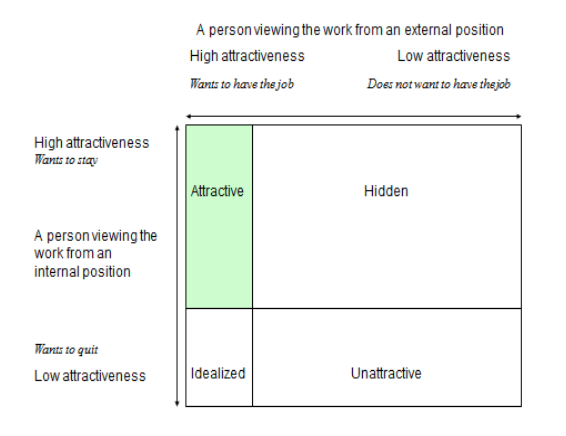
\includegraphics[width=0.75\textwidth,height=\textheight]{./media/04-attracting-young-people-to-the-mining-industry/media/image1.png}
\caption{The attractiveness of the mining industry illustrated}\label{fig:figure41}
}
\end{figure}

In fig.~\ref{fig:figure41}, we have used Hedlund's (2007) model to illustrate a plausible present situation for the mining sector. The attractive section is quite small; the view from an internal position is more positive than is one from an external position. Thus, we argue that the mining industry needs to expand job attractiveness, both for external and internal viewers (fig.~\ref{fig:figure42}). As was shown in the above models, this expansion can be achieved in many ways. Essentially, present attractive qualities must be presented and not hidden away from applicants and potential staff. Unattractive or repelling job features must be eliminated or decreased.

\begin{figure}
\hypertarget{fig:figure42}{%
\centering
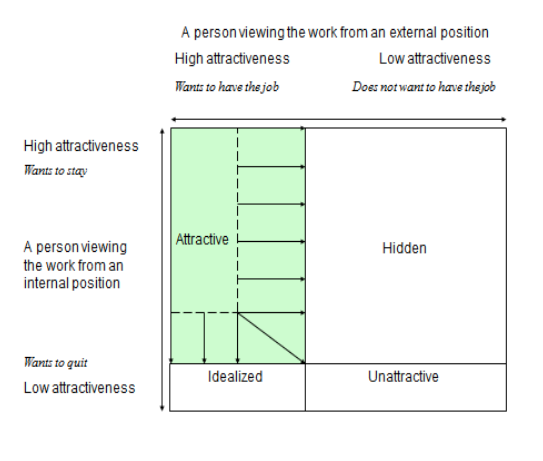
\includegraphics[width=0.75\textwidth,height=\textheight]{./media/04-attracting-young-people-to-the-mining-industry/media/image2.png}
\caption{The expanded attractiveness of the future mining industry}\label{fig:figure42}
}
\end{figure}

The question is how to achieve this expansion of attractiveness. Based on our experiences from the SIMS project and other similar projects, we have summarized our findings in six recommendations for creating attractive workplaces and increasing the visibility of the good parts of mining work:

\begin{itemize}
\item
  Health and safety at work must have top priority. Mechanization, remote control, and automation are efficient preventive safety measures but are also appropriate for reducing workload to avoid musculoskeletal injuries and allow for recovery periods. Improved safety is also a matter of a developed safety climate in the form of relevant education, rules and effective leadership where safety clearly is prioritized in the day-to-day work.
\item
  A work organization should be based on groups as an operative unit where all employees have control over their own work cycle. This very concrete demand guarantees variety at work while also providing meaningful autonomy. The demand can also be combined with a lean approach.
\item
  Competence development and learning at work are important to guarantee flexibility for the company and development in one's professional role. It is also a question of changing into a workplace culture that follows the developments in the industry, such as new production techniques, new products, and new quality demands.
\item
  Gender equality is essential for the mining industry to being viewed as a modern employer. The industry must break away from its macho-masculine image.
\item
  The mining companies must more actively demonstrate their social responsibility. Employees want to feel proud to work at the company, so issues such as vision, mission and core values are important.
\item
  Focus should be placed on the benefits and potential problems that may come with having a workforce consisting of both in-house personnel and contractors. This approach includes an emphasis on strengthening both the formal (e.g., implementing joint safety management practices) and informal (e.g., communication and interaction at the workplace level) relations at the emerging multiemployer worksites.
\end{itemize}

Finally, if the mining industry wants to improve its image and recruit young people in the future, it has to broaden its perspective. New technology is important and can solve many problems, but not all of them. Technology must be complemented with a social perspective that includes attractive and safe workplaces in a social functioning society and sought-after workplaces in a company that people are proud to work for.

\hypertarget{attractive-workplaces-do-not-fit-all}{%
\chapter{Attractive workplaces do not fit all}\label{attractive-workplaces-do-not-fit-all}}

\begin{chap-auth}
Joel Lööw
\end{chap-auth}

Thus far, we have not gone too far into the theoretical foundations of attractive work. For large parts of this book, we believe such delving to be more than is needed to use and understand the advice we advance. Nevertheless, we would like to discuss some of the less intuitive parts of attractive work and what effects these parts have on designing attractive work in a wider perspective.

We have talked about how the mining industry has a hard time recruiting labour. However, the discussion about attractive work is not only about how well organizations recruit employees. We already discussed that an organization can be attractive and still not be able to recruit workers (we have called these jobs or organizations ``hidden''). However, an organization can also be \emph{unattractive} but have no problem with recruiting the labour it needs. Think about all the workplaces with poor working conditions in which people actually work.

The model in chapter 4 (with work as attractive, unattractive, hidden or idealized) we have used in this book is useful. However, if we start to explore all the different manners in which it can be interpreted, questions start to arise. Example questions are as follows:

\begin{itemize}
\item
  Is there a difference between internal and external attractiveness? That is, will the same thing that increases internal attractiveness also increase external attractiveness (and vice versa)?
\item
  How do we balance between the many factors of attractiveness? Can negative factors be accepted if there are positive factors to compensate?
\item
  When does work go from being unattractive to attractive? If one-half of a population thinks the job is unattractive and the other half thinks it is attractive, what is the final classification? In other words, who decides whether work is attractive? Additionally, when is work attractive \emph{enough}?
\end{itemize}

We will not answer these questions definitively. However, the discussion below will hopefully help us on the way.

First, we must realize that there is a difference between what an individual considers attractive, the view of that individual of the work or workplace in question, and the actual characteristics of that work or workplace.

For example, if we had two identical individuals, where one is employed in the particular job and the other is not, they probably would not make the same judgement, because they have different ``access'' to the actual characteristics of the work or workplace. If we had two different individuals, they also likely would not make the same judgement because they have different preferences.

Additionally, the ``attractiveness'' constantly changes as preferences change. For instance, past experience, and norms and values in society, can change how we think. Therefore, perhaps the important part is not deciding whether work is attractive. Instead, we should constantly ensure that the work can change as preferences and society change.

Here, we must understand that the attractiveness is applicable not only to (potential) workers but also to designers, managers and others who form jobs and workplaces. What they (we) think is attractive will influence such decisions about what changes to make to a workplace. Moreover, the view they have of a workplace, for example, may not completely correspond to reality.

It all becomes more difficult when we consider that some aspects of attractiveness come down to personal judgement, while other parts are objectively good or bad. Let us look at an example to illustrate this point.

Blauner (1964) studied textile and automobile workers. He found that both were \emph{objectively} alienated.\footnote{According to Blauner (1964, 15), ``Alienation exists when workers are unable to control their immediate work processes, to develop a sense of purpose and function which connects their jobs to the overall organization of production, {[}and{]} to belong to integrated industrial communities, and when they fail to become involved in the activity of work as a mode of personal self-expression.''} Only the automobile workers, however, were \emph{subjectively} alienated. He argued that norms and values in the societies of the textile workers worked prevented subjective alienation.

That is, not everything a worker might prefer is good, or things are not necessarily fine because they feel fine. There are other examples. Workers occasionally prefer piece-rate wages (due to the ability to earn extra money) and extended work-hours (due to the additional days off). However, much research shows that this approach can be bad for workers' health. Moreover, organization change is occasionally resisted, for example, when implementing measures for increased equality. That they are resisted does not necessarily mean that they are bad.

Thus, although we previously discussed the views of employees forming work, we must also ensure that we are knowledgeable about many different aspects of work.

What does the above mean for designing attractive work? At the very least, it means that participation from workers is absolutely necessary. Attractive work cannot be designed from behind a desk. Today, it is quite common to talk about user-centric design. However, if we are serious about attractive work, we must go further. We must ask even those who will not work in the jobs we are designing. Societal norms and values will influence what we think of particular jobs. If we do not take this point into consideration, it may not matter how well we design jobs -- they still can be considered unattractive.

However, we cannot leave it all up to opinion. In fact, all of us who make decisions that influence work must better our understanding of work and how our actions influence it.

This book is about technology and its social acceptance. With our discussion here, we can say that the design of technology is ongoing work. Even when a design is finished, a product delivered and so on, it will need attention. Because ``society''---humans---change all the time, technology must adapt.

\hypertarget{meeting-social-challenges-in-established-mining-communities}{%
\chapter{Meeting social challenges in established mining communities}\label{meeting-social-challenges-in-established-mining-communities}}

\begin{chap-auth}
Eugenia Segerstedt
\end{chap-auth}

In this chapter, we will broaden the frame of reference and discuss the mining industry's responsibility to operate in a socially sustainable society. By ``established mining communities'', we mean communities that co-exist with ongoing mines and mining companies. In Sweden, these communities are often rural and small or midsized towns.

Such towns face many practical challenges that provide both possibilities and obstacles to supporting socially sustainable development, challenges that they in varying degrees share with mining communities in countries such as Norway, Finland, Australia, and Canada. Many of these communities have always been, and indeed still are, at the mercy of global market fluctuations in the mining, steel, and forestry sectors. They are situated in districts that are home to highly valued natural areas, major tourist attractions, and mixed populations where indigenous peoples are an important presence; in some cases, these areas are sources for important and difficult discussions and debates, and occasionally even overt conflicts. Examples of deep-rooted and persistent problems in these communities include the following: low education levels (especially among men), depopulation (as women and young people move away), economic stagnation, downsized welfare services, a low level of activity in other sectors (trade, housing, communication, and infrastructure), and a gender-segregated labour market with a low degree of differentiation. Those two last aspects distinguish industrial communities from small rural communities. In addition, these areas are often characterized by a social construction of rural citizens (especially men) as ``old fashioned'' and culturally conservative.

The problems outlined above are undoubtedly substantial, but some of them are offset by periods of more positive trends such as a low level of unemployment, new investments in housing and infrastructure, and growing entrepreneurial activity. Many of those challenges are relevant for rural industrial communities, but some are specific to mining communities. In periods when mining is booming, the problems change character and become related to, for example, lack of housing and infrastructure and the difficulty in recruiting new employees with the right skills, both for the mining companies and other ancillary businesses and welfare services such as healthcare. Other major challenges relate to the environment, more specifically, to how to balance the mining companies' need for efficient licensing with environmental concerns. Moreover, even if we can see an emerging diversity of livelihoods, the recent mining boom mainly led to an increase in activity in businesses and industries that have long been dominated by men.

Aspects of urban life in established mining communities such as social cohesion and inclusion, migration and demographics, good housing infrastructure, and gender equality can enable (or disable, in a figurative sense) diversity of livelihoods in those communities. A strong community identity can be seen as good grounds for social cohesion, but at the same time, this result can be associated with a certain lifestyle that is not inclusive, for example, if this lifestyle has a connection with traditional (specifically rural and mining worker) masculinity. Concerning social cohesion and inclusion, some studies focus on the local community with respect to decision-making processes (e.g., issuing a ``social license to mine''). Swedish studies of mining communities discuss strong community identity, which can be seen as promoting cohesion, but as alluded to above, this identity is often associated with a certain lifestyle that is not inclusive and is characterized by ``traditional masculinities''. Some international studies have also found mining communities to be notably cohesive internally, but local networks were not considered strong \emph{and} inclusive.

Crawley and Sinclair (2003) have examined how to broaden a mining company's recruitment base by including indigenous people, a strategy based on power sharing. The conclusions in the study placed high hopes on the UN declaration on the Rights of Indigenous People that was being discussed at the time of the study and that was adopted later in 2007. One might argue though that the UN declaration lacked the ability to alter the normative environment for mining companies. Indeed, the aftermath of the declaration proved to be something of a disappointment because it became clear that it did not---perhaps could not---change things anywhere near enough for indigenous people; rather, positive advances would, as so often in the past, come from local pressures exerted and directed from below. There is an undeniable ambition to preserve indigenous peoples' cultural expressions. Australian and North American studies have examined how the mining industry has negatively affected indigenous people by severely limiting their ability to practice their traditional lifestyle. The concern is often with indigenous peoples' rights and access to prior, free, and informed consent to mine, for example, as these issues relate to international law.

The practical implications of these challenges are the following:

\begin{itemize}
\item
  Measures towards community cohesion might be problematic.
\item
  Social licensing should be a continuous process, a dialogue between the mining company and the established mining community.
\item
  Working towards a less gender-segregated local labour market is essential.
\item
  It is important to work for indigenous peoples' rights and access to prior, free, and informed consent to mine.
\end{itemize}

\hypertarget{risk-analysis-and-prevention}{%
\chapter{Risk analysis and prevention}\label{risk-analysis-and-prevention}}

\begin{chap-auth}
Jan Johansson and Bo Johansson
\end{chap-auth}

A heavy responsibility for safe mines lies on the mine planners' shoulders. They must find solutions that promote high productivity and good economy and safety and a healthy work environment. The mine planners will initially shape the general and specific work environment for miners for many years to come. If the planners design a poor solution and it is necessary to redesign it, it will also probably be very expensive to correct after it has been implemented.

Work environment and safety issues are unfortunately often left quite unattended in the early stages of mine planning and design when they instead should be systematically highlighted and developed from the very first planning steps. The best and most efficient means of gaining safety is through proactive planning rather than through reactive corrective actions. It is also the best approach to reducing the associated costs for risk elimination and reduction.

The mine planner is, however, not alone; he or she works in a company context where safety climate and culture, safety policy and safety management have a strong influence on how well the planner can succeed in his or her work.

The slogan ``safety first'' has been heard in the mining business for many decades but is still in many cases no more than a slogan, since safety first is not fully practised, especially if the business has financial problems. It seems, however, that times are changing and that many mining companies are now making great efforts to improve their safety climate and safety culture. Research on safety has shown that a positive safety climate and well-developed safety culture are important requisites for a healthy and safe work environment, especially in heavy industries.

To manage the risks in the business, every mining company also needs a strategic long-term policy regarding how to deal with safety issues and strive for better work conditions. The safety policy should direct and establish systematic ways to manage (plan, steer and control) the safety work, including early planning and design activities.

Because mining is a very risky business, it has to follow and obey many directives, laws and provisions. Most of these rules only stipulate minimum demands; the companies are free to exceed them. This approach is also what mine planners should aim at, i.e., exceeding minimum demands. A first step for a mine planner is therefore to become acquainted with the national and international (i.e., EU regulations) system of rules and basic demands. Many of these demands are provided by the national or EU authorities, a task that must be done thoroughly in each country; there are quite a large number of directives, laws and provisions that regulate and give guidelines for health and safety issues in underground mining.

The basis for all activities in systematic health and safety work should always be an initial, thorough risk assessment of both the present state and a future planned state. It is of course easier to assess present or historical risks than future risks, especially if the future holds large changes in technology and or work organization. Nevertheless, a mine planner needs to assess the risks associated with different mining concepts that are developed and planned.

Mining might develop in a revolutionary way, but it will most likely develop in another way, in an evolutionary way. In other words, much can be learned from history and from the present state. Thorough evaluations of present and historic designs have for example systematically been used by the Swedish mining company LKAB in the design of their newest main level at 1365 m below the surface. This evaluation has been very important, since the time span from the first conceptual designs to the final solutions has stretched over 12 years and many planners.

Risk assessments can be performed in number of ways, depending on the situation and circumstances. All risk assessment should however be based on probability and consequences of unwanted events. A practical tool for this purpose is a risk matrix that eases a systematic and consequent risk assessment; see fig.~\ref{fig:tablea}

\begin{figure}
\hypertarget{fig:tablea}{%
\centering
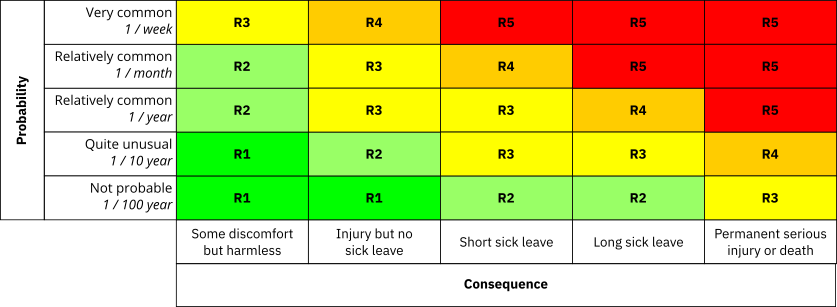
\includegraphics{./media/tab-matrix.png}
\caption{Risk matrix based on probability and consequences.}\label{fig:tablea}
}
\end{figure}

As seen in fig.~\ref{fig:tablea}, probability is expressed as a frequency for a specific event or deviation. During planning, the assessed risk level can also be coupled to a specified need for action; see fig.~\ref{fig:tableb}

\begin{figure}
\hypertarget{fig:tableb}{%
\centering
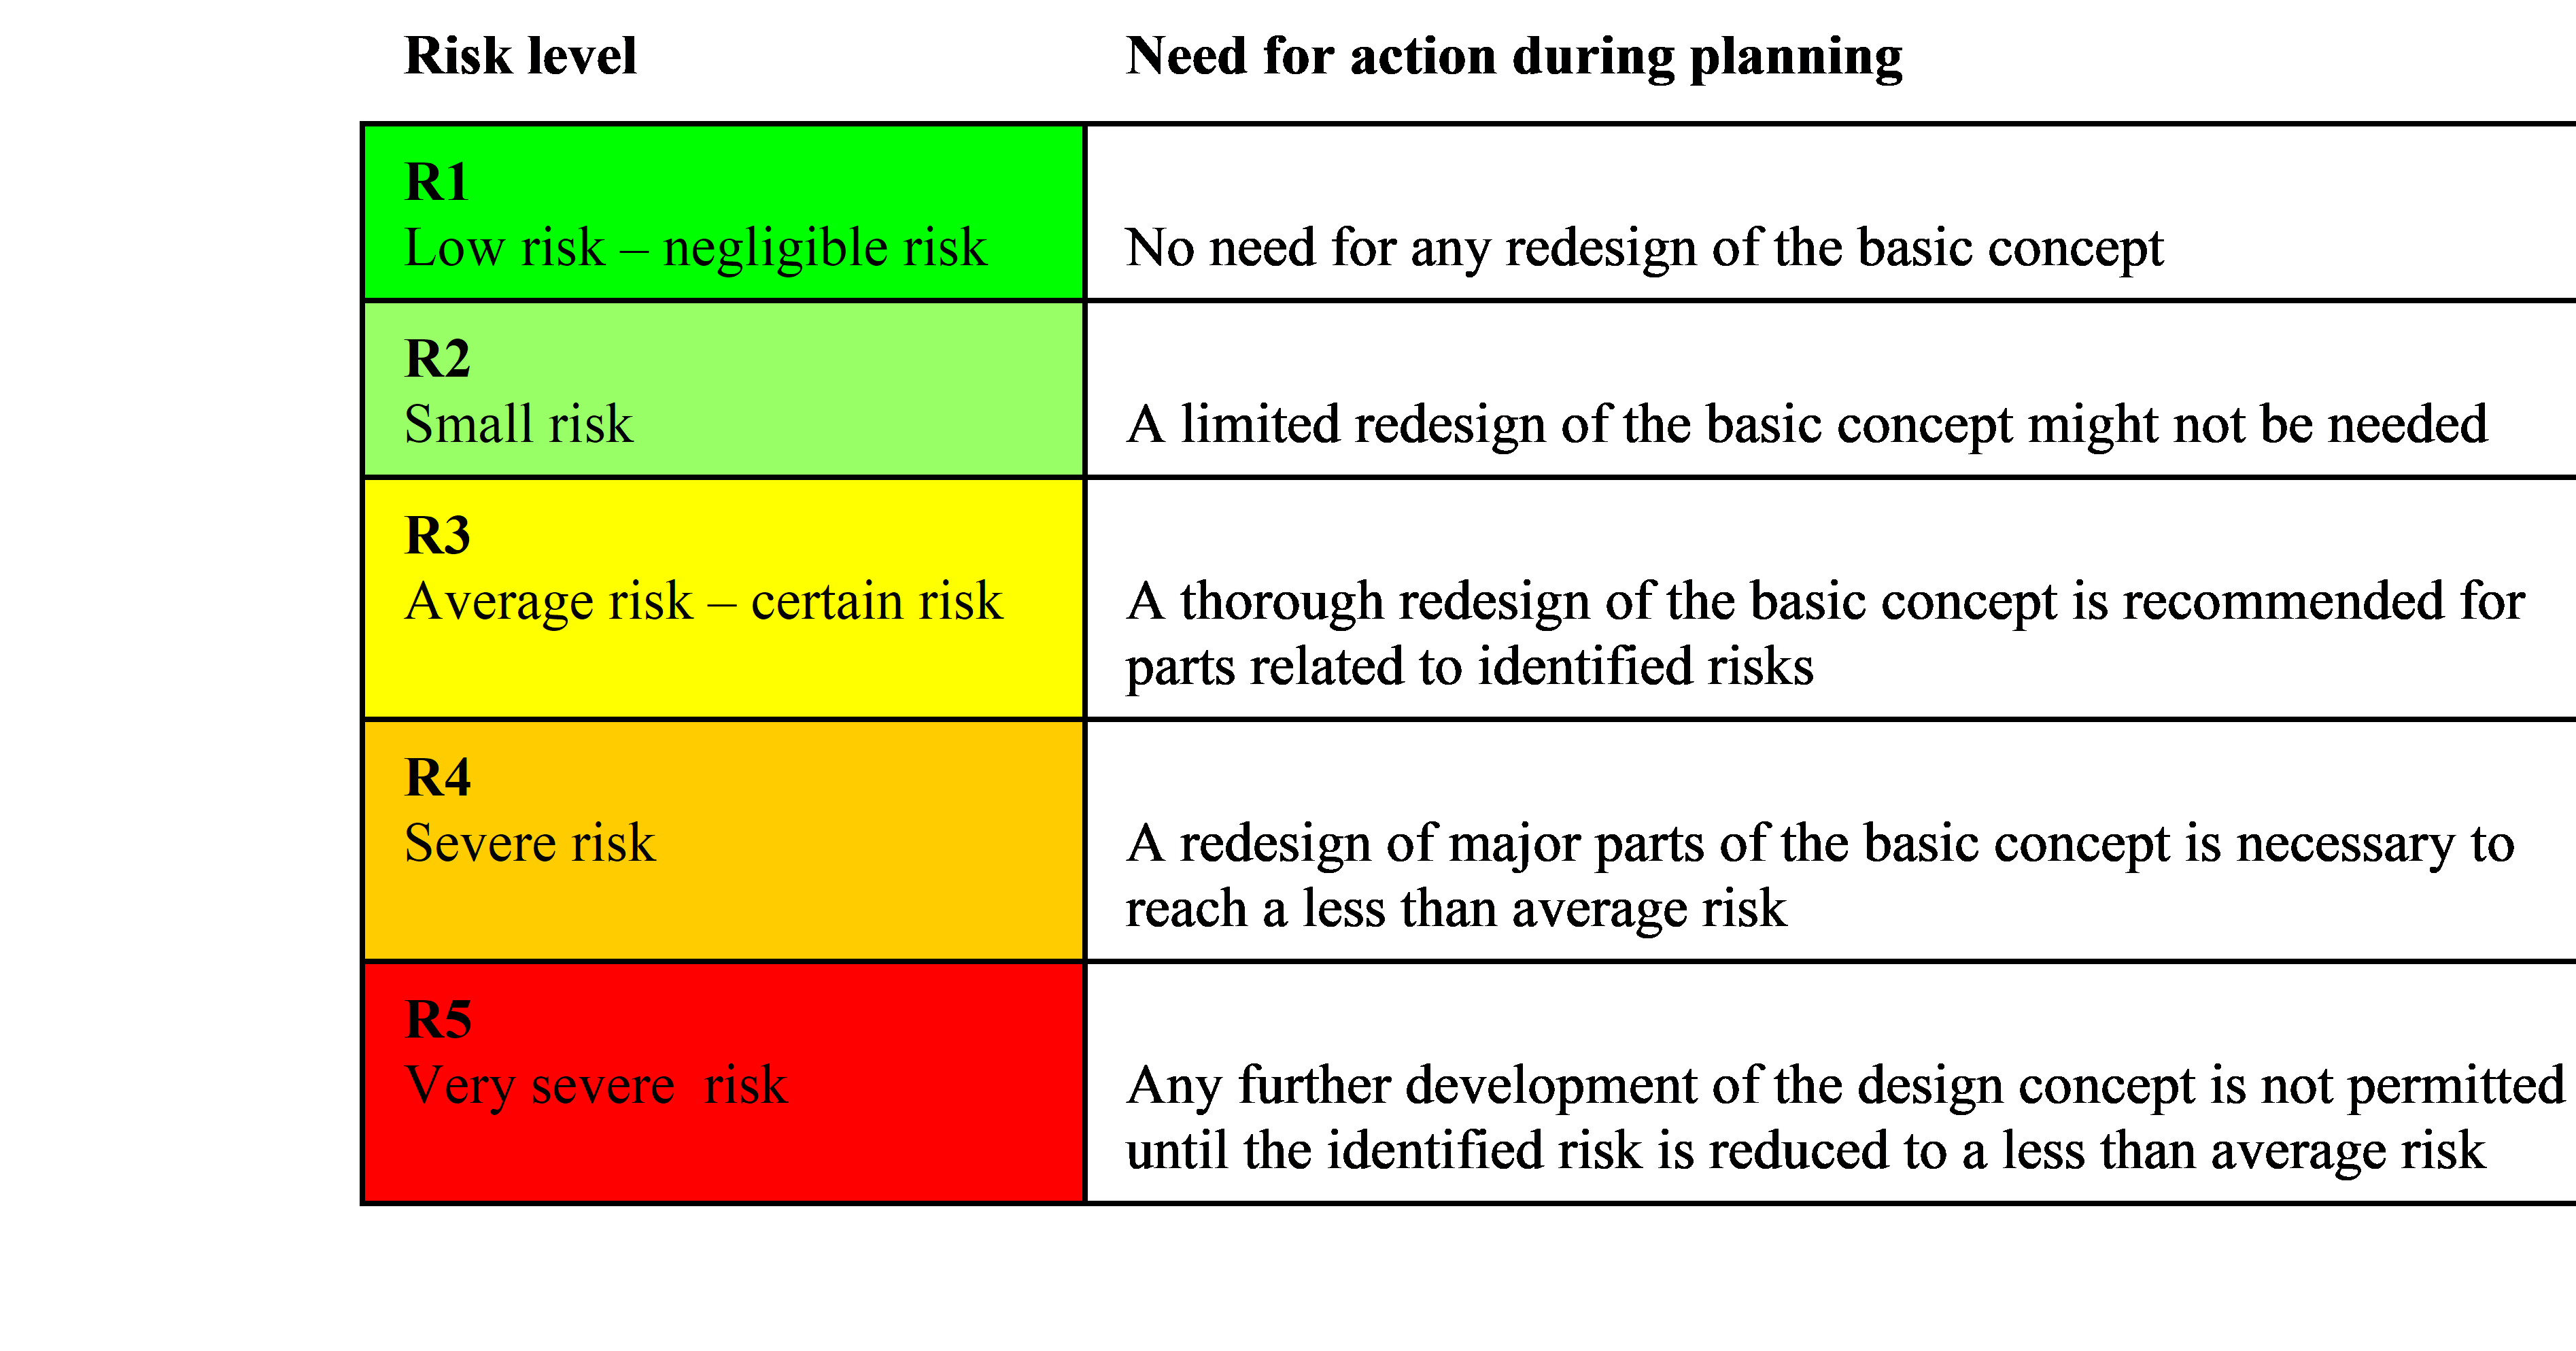
\includegraphics{./media/risk-level-planning.png}
\caption{Risk level and need for action during planning.}\label{fig:tableb}
}
\end{figure}

The risk matrix for risk assessments during planning can also, with some modification, be used for risk assessments in the operative production stages (fig.~\ref{fig:tablec}). The risk matrix has therefore become a quite well known and used tool in mining companies.

\begin{figure}
\hypertarget{fig:tablec}{%
\centering
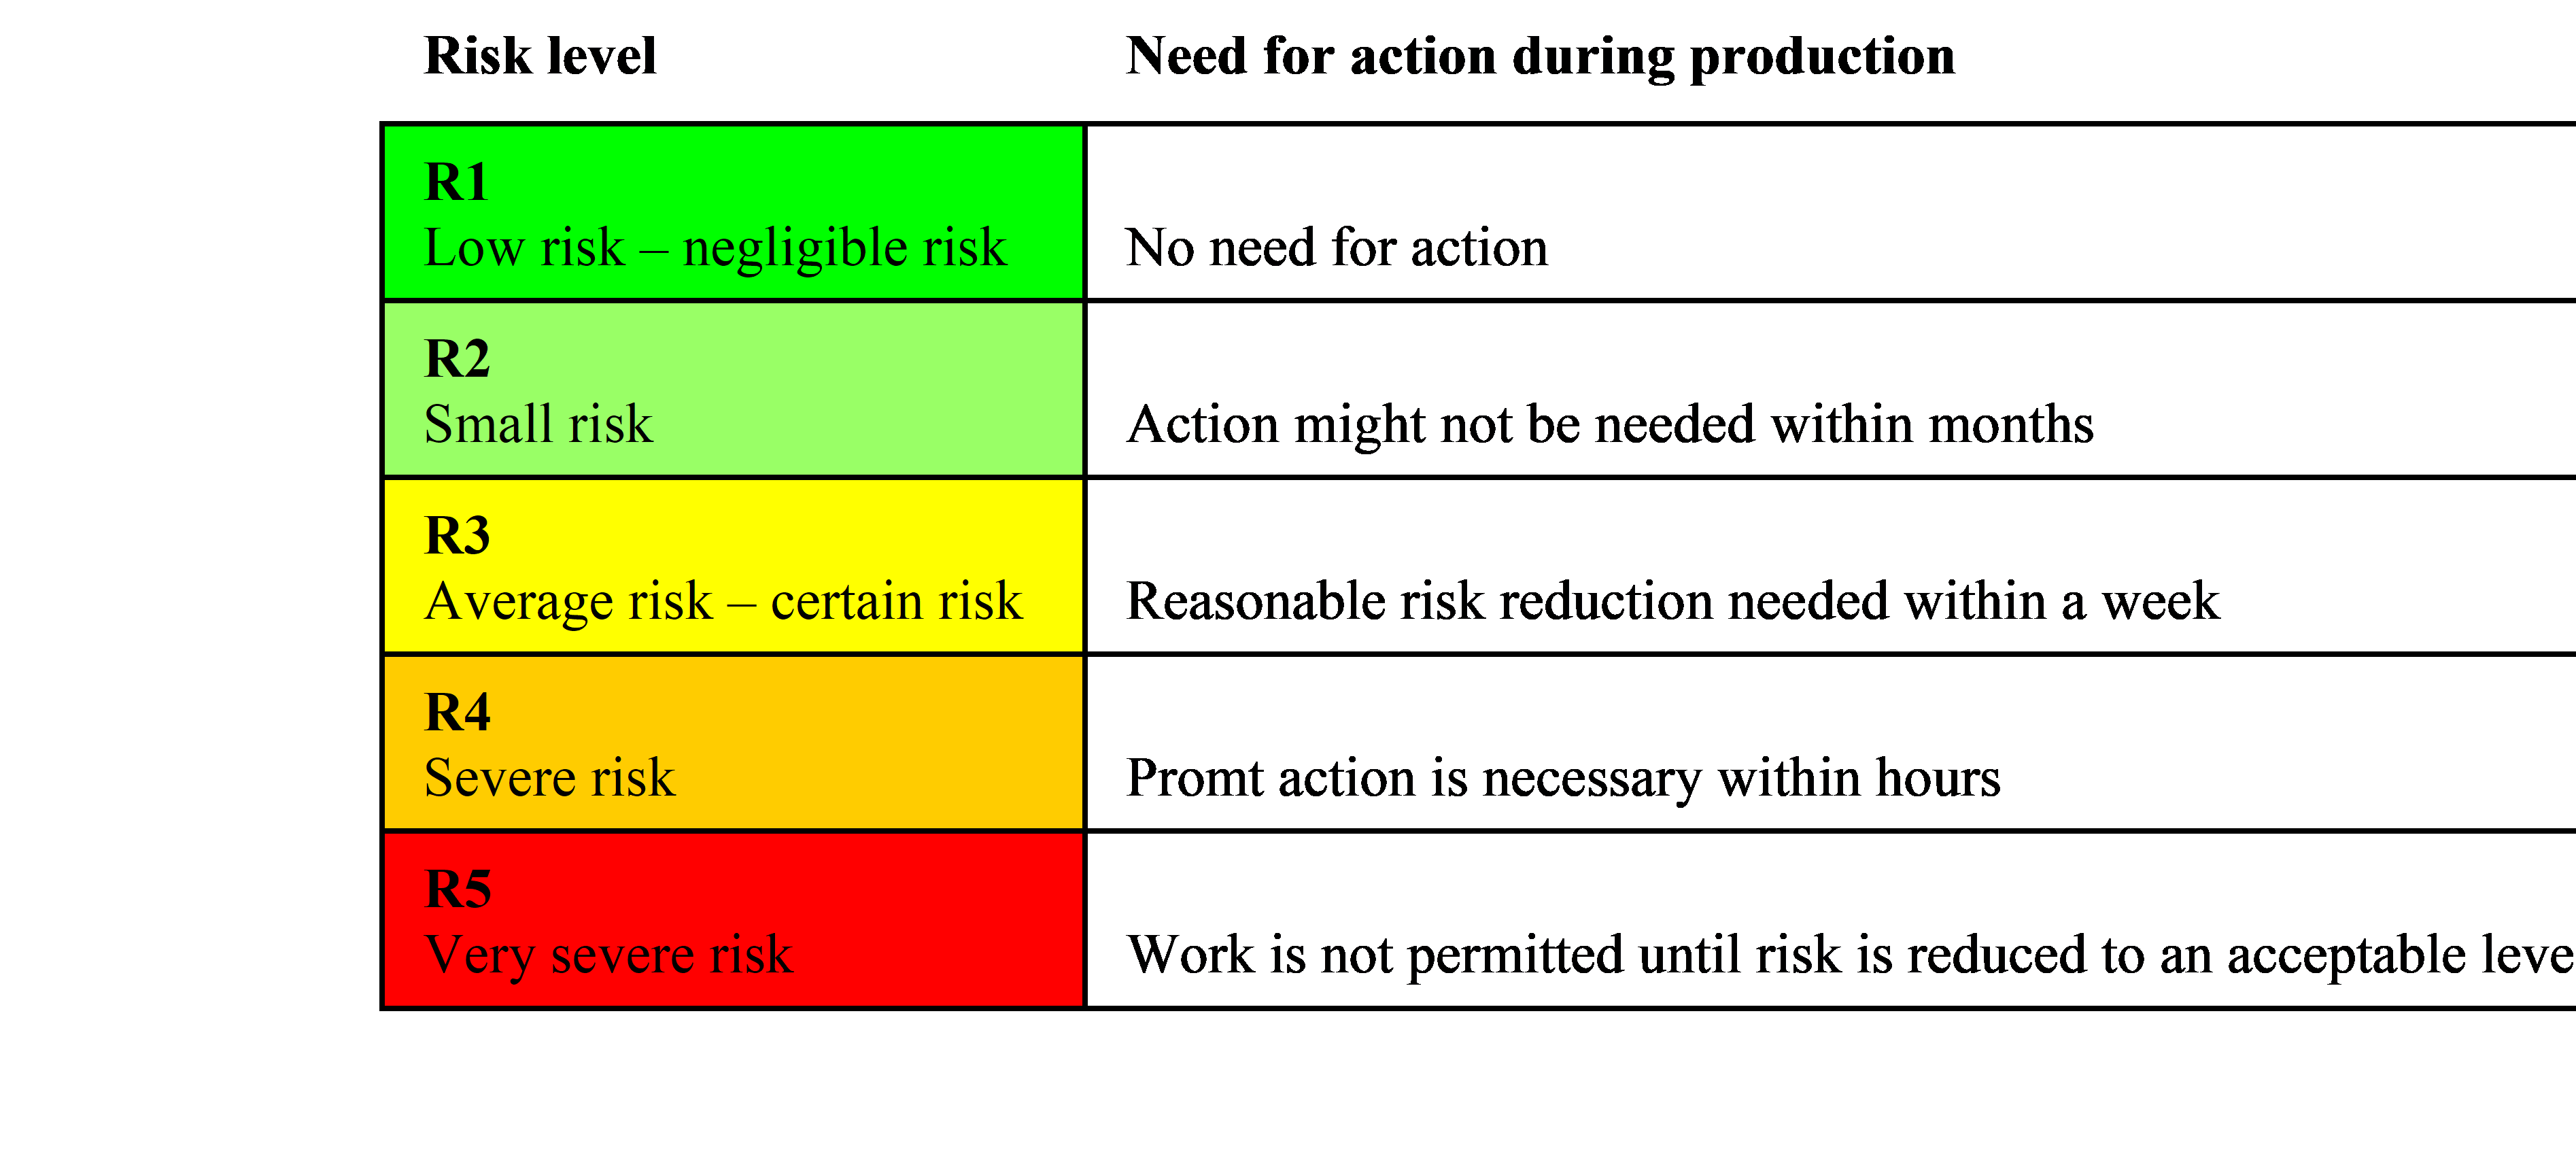
\includegraphics{./media/risk-level-production.png}
\caption{Risk level and need for action during production.}\label{fig:tablec}
}
\end{figure}

The classical tools for the identification of occupational risks in the existing production environments are safety rounds, incident reporting and accident reporting. These tools are however less suitable to identify and assess risks in future work environments. These environments require other types of more proactive methods such as the following:

\begin{itemize}
\item
  Preventive deviation analysis
\item
  Preventive energy analysis
\end{itemize}

According to Harms-Ringdahl (2013), a deviation is defined as an event or condition that deviates from the intended or normal. The purpose of a deviation analysis is to predict and prevent abnormalities that can cause damage and to develop proposals to improve safety measures. Deviation analysis is a very useful method, since it takes into account the entire system, human-technology organization. Energy analysis focusses more on technology and might be useful when developing new productions systems. The three main components considered in an energy analysis are the following:

\begin{itemize}
\item
  Energy that can damage
\item
  Targets that may be harmed
\item
  Barriers to energy
\end{itemize}

The energies usually considered are the following: gravity, height (including static load), linear motion, rotary motion, stored pressure, electrical energy, heating and cooling, fire and explosion, chemical effects, radiation, and miscellaneous (human movement, sharp edges, and points).

There are also many other different risk analysis methods that can be used in the development of new production systems. In addition to the methods mentioned above, methods such as preventive work safety analysis (PWSA), failure mode effect analysis (FMEA), fault tree analysis (FTA), event tree analysis (ETA), and work environment screening tool (WEST), etc., can be used. The most appropriate tools have to be chosen for every specific analysis task, and the users of the tools must also have the necessary competence to attain reliable and relevant results. Here, the mining business probably can learn much from other industries that have strong safety cultures and long experience of systematic risk management. Especially important will be to learn how to proactively manage risks for fatalities and other severe risks. Here, so-called leading indicators are preferred instead of lagging indicators.

Although there are many risk-evaluation tools available, the mining industry seems to need new and efficient tools for description, evaluation and design of work environments during early phases of strategic decision making and production system design. The most important decisions regarding work environment and safety are made by top management when mining methods, technology, and work organization, etc., are decided. Therefore, risk analyses regarding these matters should be performed as early as possible in the mine design process.

Once a risk analysis is completed, it often requires measures that in most situations should be implemented in the following well-known order:

\begin{enumerate}
\def\labelenumi{\arabic{enumi}.}
\item
  Prevent in the planning stage; replace the hazards entirely, for example, through automation to eliminate manual or mechanized underground work.
\item
  Isolate the individual hazard or risk process, for example, by designing ventilation and layout so that blasting fumes cannot be spread outside the risk zone.
\item
  Change process technology and behaviour; for example, employ DTH-drilling with water hydraulics rather than pneumatics to reduce dust emissions.
\item
  Limit the hazard through enclosures and physical protection. For example, build concrete borders and railings at the shaft openings.
\item
  Isolate personnel from the hazard risk area, for example, by supplying the mining vehicles with safety cabs with good climate control.
\item
  Risk is reduced by instructions, procedures, and training, etc., with, for example, procedures for safe handling of explosives.
\item
  Risk is reduced through personal protective equipment, for example, functional working clothes.
\end{enumerate}

Depending on the complexity and severity of problems, one may require different combinations of measures as described above. One recommendation is to always try to attack the root causes of the problem first. This approach tends to result in the most cost efficient and result-efficient solutions. This task is important for mine planners. They have the best opportunity to eliminate many potential health and safety problems when they develop the first conceptual solutions. Planners that do not realize this point and neglect these matters can cause great harm for many years to the mining personnel and their company.

\hypertarget{safe-and-attractive-workplaces-for-contractor-personnel}{%
\chapter{Safe and attractive workplaces for contractor personnel}\label{safe-and-attractive-workplaces-for-contractor-personnel}}

\begin{chap-auth}
Magnus Nygren
\end{chap-auth}

It is common practice in the contemporary mining industry to hire contractors to perform certain work tasks. This approach has led to the emergence of multiemployer worksites where workers from different companies are active in close proximity to one another. This situation poses specific challenges concerning health and safety and, by extension, work attractiveness. Workplace accidents, in particular, have historically been a problem in relation to outsourcing and contracting. Muzaffar et al.~(2013) show that the odds for contractor employees sustaining a fatal injury while performing work in the US mining industry were almost three times higher compared with those of the mining companies' own personnel. In the Swedish mining industry, contractor workers have likewise regularly had higher accident rates in recent years (Svemin, 2010). The matter of certain groups of workers potentially having an increased risk of suffering accidents is important to address in its own right. However, such a risk is also important to consider from the perspective of recruitment and ensuring work attractiveness.

In a literature review of research on safety at multiemployer worksites, Nygren et al.~(2017) propose that several key concepts and terms can be found and divided into three overlapping categories (tbl.~\ref{tbl:tablex}).

\hypertarget{tbl:tablex}{}
\begin{longtable}[]{@{}lll@{}}
\caption{\label{tbl:tablex}Examples of key concepts and terms (Nygren et al., 2017)}\tabularnewline
\toprule
\begin{minipage}[b]{0.31\columnwidth}\raggedright
Category\strut
\end{minipage} & \begin{minipage}[b]{0.27\columnwidth}\raggedright
Key concepts and terms\strut
\end{minipage} & \begin{minipage}[b]{0.33\columnwidth}\raggedright
\strut
\end{minipage}\tabularnewline
\midrule
\endfirsthead
\toprule
\begin{minipage}[b]{0.31\columnwidth}\raggedright
Category\strut
\end{minipage} & \begin{minipage}[b]{0.27\columnwidth}\raggedright
Key concepts and terms\strut
\end{minipage} & \begin{minipage}[b]{0.33\columnwidth}\raggedright
\strut
\end{minipage}\tabularnewline
\midrule
\endhead
\begin{minipage}[t]{0.31\columnwidth}\raggedright
Contract work characteristics\strut
\end{minipage} & \begin{minipage}[t]{0.27\columnwidth}\raggedright
\begin{itemize}
\item
  High workload
\item
  Insufficient training
\item
  Low autonomy and task demand
\item
  Normalization of risk
\end{itemize}\strut
\end{minipage} & \begin{minipage}[t]{0.33\columnwidth}\raggedright
\begin{itemize}
\item
  Time constraints
\item
  Temporary and/or peripheral work
\item
  Unfamiliarity with work environment
\end{itemize}\strut
\end{minipage}\tabularnewline
\begin{minipage}[t]{0.31\columnwidth}\raggedright
Structural/organizational factors and conditions\strut
\end{minipage} & \begin{minipage}[t]{0.27\columnwidth}\raggedright
\begin{itemize}
\item
  Communication barriers
\item
  Disorganization effects
\item
  Substandard division of responsibility
\end{itemize}\strut
\end{minipage} & \begin{minipage}[t]{0.33\columnwidth}\raggedright
\begin{itemize}
\item
  Ineffective and insufficient information sharing
\item
  Unstable social relations
\end{itemize}\strut
\end{minipage}\tabularnewline
\begin{minipage}[t]{0.31\columnwidth}\raggedright
Cultural conditions\strut
\end{minipage} & \begin{minipage}[t]{0.27\columnwidth}\raggedright
\begin{itemize}
\item
  Cultural integration difficulties
\item
  Culture of independence
\item
  Differing norms and values
\end{itemize}\strut
\end{minipage} & \begin{minipage}[t]{0.33\columnwidth}\raggedright
\begin{itemize}
\tightlist
\item
  Macho-masculine work culture
\end{itemize}\strut
\end{minipage}\tabularnewline
\bottomrule
\end{longtable}

As seen, research on the subject mainly highlights the safety-related problems that arise when contractors are hired, rather than the benefits that multiemployer arrangements may bring. Consistent with Mayhew et al (1997), Nygren et al.~(2017) argue that many of the problems can be connected to two main factors:

\begin{enumerate}
\def\labelenumi{\arabic{enumi})}
\item
  Economic pressures
\item
  Disorganization
\end{enumerate}

The first factor, \emph{economic pressures}, highlights that contractors (and in particular smaller companies) may not invest in health and safety-related matters due to a lack of resources. This factor includes less systematized management practices and a lack of comprehensive safety education and training. The second factor, \emph{disorganization}, focusses on the organizational conditions for safety. Multiemployer worksites are often characterized by complex contracting chains, with contractors hiring other (sub)contractors, or multiple contractors being hired by a mining company for different projects. This situation can lead to unclear relationships between groups of workers, ambiguity in the organization of work, and a breakdown in communication and substandard division of management responsibilities.

Given that mining companies are relying on contractors to a significant extent, the concept of work attractiveness should be expanded to also include the conditions that arise in multiemployer arrangements. The following points can be taken into consideration when aiming to increase safety in these types of work setting and, by extension, work attractiveness for contractor personnel:

\begin{itemize}
\item
  The mining company should ensure that the contractors have well-functioning health and safety management systems in place, including a clear division of roles and responsibilities.
\item
  Safety education and training should be a prerequisite for conducting work in the industry, regardless of employer. This prerequisite should also be documented in the form of, e.g., certificates of completed courses.
\item
  The work needs to be scheduled carefully, include realistic time frames, and communicated clearly to everyone involved, including the mining company informing the contractors of any/all adjacent work by other companies that will be conducted simultaneously.
\item
  Meetings should be organized where health and safety-related issues are discussed as a means of encouraging risks and hazards to be shared between companies and between workers. The responsibility for organizing these meetings should lie on the party that owns and oversees the operation in question, i.e., representatives from the mining company itself.
\item
  It should be possible for contractors to report safety-related incidents to the mining company's own safety database. It should also be possible to hand in observed risks and hazards manually through, e.g., specific ``mailboxes'' placed in and around the operations.
\item
  Post-work evaluations should be performed on how health and safety issues have been handled by the contractors and by the mining company itself, including the communication and information sharing between the parties involved.
\end{itemize}

\hypertarget{understanding-and-improving-safety-culture}{%
\chapter{Understanding, and improving, safety culture}\label{understanding-and-improving-safety-culture}}

\begin{chap-auth}
Magnus Nygren
\end{chap-auth}

Safety work has evolved over time in the mining industry. In the 1980s and 1990s, a focus was to a significant extent placed on technological solutions such as improved protection from hazards related to blasting and safer and more efficient machinery. New laws and regulations have also come into effect in recent decades that have led to more systematized risk management practices overall. Although technological solutions and the implementation of formal rules still play an important part, there has been a trend towards finding more-novel organizational solutions for safety-related issues. One such solution is improving the \emph{safety culture} within the companies.

Safety culture can be defined as the ``shared and learned meanings, experience and interpretations of work and safety---expressed partially symbolically---which guide peoples' actions towards risks, accidents and prevention'' (Richter \& Koch, 2004, p.~705). In practice, improving safety culture often involves a focus on encouraging safe behaviours, including the introduction of new procedures that are seen as facilitating certain types of behavioural practices. However, safety culture is a complex phenomenon that also involves interactions and exchanges among the workers themselves; i.e., safety culture emerges in a ``bottom-up'' fashion and may establish worker-specific norms and values that are outside of the direct control of management.

The notion of safety culture being something that both management can improve and something that evolves naturally among the workers themselves is succinctly encapsulated in a model by Edwards et al.~(2013) (fig.~\ref{fig:figure91}).

\begin{figure}
\hypertarget{fig:figure91}{%
\centering
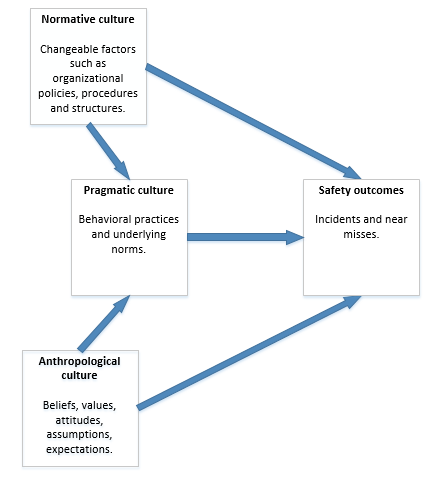
\includegraphics{./media/10-understanding-and-improving-safety-culture/media/image1.png}
\caption{Model of safety culture (Edwards et al., 2013)}\label{fig:figure91}
}
\end{figure}

Safety outcomes can thus be seen as being dependent on three different ``types'' of culture that interact with each other in complex ways -- or rather that three different perspectives can be used on the nature and characteristics of culture. Normative culture highlights that specific structures, policies and procedures will make certain behavioural practices more likely to occur (i.e., pragmatic culture) that, in themselves, are affected by the beliefs, values and expectations of the workers (i.e., anthropological culture). However, while taking the interconnectedness of the three perspectives into account, a dedicated focus by management on implementing appropriate structures, policies and procedures is clearly a promising avenue for cultural change. One reason for this promise is that the formal structures and processes of an organization are under the direct control of management and, consequently, something that can be fairly easy to change, which eventually may have an effect on the meaning workers ascribe to safety. For example, Guldenmund (2010) suggests that the safety management system of an organization may play an important part in creating meaningful safety practices for the workers by, e.g., making clear what is expected of them in their daily work. Nevertheless, it is also important to consider how new initiatives will be perceived and interpreted by the workers given that the culture, in the anthropological sense described above, can be seen as something ``belonging'' to the members of the organization themselves. If the suggested changes to policy and procedures are not consistent with what the workers expect and need, there may be a resistance to change or, in other words, a clash between cultures. Of course, some policies and procedures may be non-negotiable, for example wearing personal protective equipment and following safety rules, but it is important to reflect on the actual consequences that management-led initiatives will have from a cultural perspective.

As seen, safety culture is a complex phenomenon, and there are no easy solutions or implementation strategies. The literature, however, offers additional considerations for mining companies when they are seeking to develop their culture:

\begin{itemize}
\item
  It is important to consider cultural issues in relation to other vital aspects of workplace safety, such as the current and future levels of technology development. Mining companies operate in conditions of intricate technical, physical and organizational relationships; everything is connected to everything, and it is important to consider both ``soft'' (e.g., safety culture) and ``hard'' (e.g., technology development) perspectives on safety (Lööw \& Nygren, 2019).
\item
  Cultural change may require several years, even decades, to come into effect (Guldenmund, 2010); thus, management needs to take this requirement into account when developing and implementing new structures and processes aimed at supporting the development of safety culture.
\item
  If a mining company hires contractors, it is important to consider how the workers of these external companies can be integrated into the structures and processes of the mining company and the level of integration that is appropriate given the formal division of responsibilities between different employers (Lööw \& Nygren, 2019). A reasonable start could be to synchronize the safety management systems of every company involved with that of the mining company. Cultural integration, in itself, may not be possible or even desirable due to the often-short-term projects contractors are hired to perform. However, introducing the workers to the context for safety work can clarify what kind of meaning should be placed on safety and that it is everyone's responsibility to act accordingly.
\end{itemize}

\hypertarget{gender-and-gender-equality}{%
\chapter{Gender and gender equality}\label{gender-and-gender-equality}}

\begin{chap-auth}
Lisa Ringblom
\end{chap-auth}

The mining industry is exceedingly male-dominated. Globally, the workforce consists of approximately 90 per cent men but with great variation depending on country, mineral and company. In the world's top 500 listed mining companies only seven of these have a woman as CEO and about eight per cent of board representatives of these companies are women. Although mining has a significant history as work for and by men, this has not always been the case. A historical perspective on mining shows that the mine and its workplaces have not always been an arena solely for men. Depending on time and geographic location in history women have participated in all areas of the mining process. For example, in Sweden before the industrialization the number of women were at some mines as high as 55 per cent of the workforce. Due to the changes that came with the industrialization a statutory ban on women in underground work was implemented in 1900, a law that was repealed first 1978. The ban on women underground followed a more general ideological shift of societal norms that took place during industrialization, which affected the relationship between men and women. With the development of a stronger division between paid and unpaid work, a women's place was first and foremost seen as the one as a wife and mother and women's salaried employment was predominantly seen as a complement to that of men. The exclusion of women in mining is not unique to Sweden, but is also found in other national contexts such as the United Kingdom, China and Peru. The reason for women's more or less temporary exclusion from mining work at different times in history has been legitimated with all from superstition (e.g.~beliefs concerning misfortune with women underground) to national structural changes.

The mining industry is not only male-dominated but also characterized by masculinity. Traits that traditionally have been labelled masculine, such as being strong, brave, and tough, etc., are still ideals within mining. A ``macho-masculinity'' has to a large extent ruled structures, practices and procedures for the blue-collar working professional and professional ideals of mining. This type of macho-masculinity, associated with characteristics that are largely related to a physical body, such as practical knowledge, physical strength and endurance under stressful and risky working conditions, have connections to increased risk-taking, which in mining can have devastating outcomes for organizations but primarily for the individual in terms of injuries and ultimately death. Research on the link between gender and safety work in the mine has shown how the idealized macho-masculinity premise of risk-taking poses a potential safety risk at work. These conservative ideas concerning gender can also be problematic during organizational and technological change and can create implementation problems and restoration responses. Because of the male dominance and the idealized macho-masculinity, mining organizations risk conflating gender with competence, something that can function as an effective exclusion mechanism in these workplaces for those who are not perceived as fitting the norm of a ``real'' mineworker, i.e., women. The historical exclusion of women from mining work, the dominant ideal of macho-masculinity, and men's numerical dominance has created an opportunity for constructing women as deficient and deviant in relation to mining. This construction has contributed to the fact that women have not been able to participate in mining work under the same conditions as men and is expressed through, for example, stereotyping and sexualization of women. Sexism, sexual harassment and discrimination are recurring themes in women's working life in the mine.

Although men and macho-masculinity dominate mining, when gender and gender equality is actualized in the mining industry, it tends to focus on women. For example, when a mining organization raises gender as an issue, it is commonly the (often) low proportion of women that tends to be in focus. This issue is of course an important question to increase women's participation in mining and to have the benefits of mining be more equally distributed between men and women. However, focussing only on the number of women is not the entire solution for the male bias in the mining industry. Women should not only have the opportunity to enter but also want to stay in the industry. To increase gender awareness and to improve gender equality demands more from organizations than counting heads. In other words, more-qualitative measures that focus on the terms for men and women in the industry also need to be implemented, that is, actions that challenge the unequal structures that do not necessarily change with an equal distribution of women and men. To have a gender perspective and to work for increased gender equality does not mean a sole focus on women; men are not to be left out of the equation.

What is understood as ``appropriate'' work for men or women is not a law of nature; it is possible to change, as are organizational cultures and the degree of diversity in the workforce. A long-term responsibility and commitment towards a socially sustainable development in mining needs to take gender issues into account in a broad range of ways, concerning both organizational issues and the gendered implications for the surrounding communities. Issues for women in the work environment in male-dominated organizations are usually an indication that the work environment is not healthy for anyone. Even if women are especially exposed in a male-dominated workplace, there are good reasons to believe that the work environment is problematic for all.

\begin{itemize}
\item
  Gender equality means that women and men have the same rights, responsibilities and opportunities in all areas of life. So, gender is not a women's issue. Gender equality concerns \emph{both} women and men.
\item
  In a male-dominated industry as mining, to attract and recruit (more) women is an important step towards improved gender equality. \emph{But}, to just focus on the number of women entering the industry is not enough. For example, women could be entering \emph{and} leaving the industry within a short period of time which means that both in-flux and out-flux are important aspects. Most importantly however, is to analyze and examine the organizational terms and conditions for women \emph{and} men within the organization. To increase gender equality in a sustainable and long- term way demands knowledge, time, resources and systematic work.
\item
  At last, changing the question could lead to other solutions. Instead of asking why there are few women working within the mining industry, a maybe more interesting question would be -- Why is there so many men?
\end{itemize}

\hypertarget{can-technology-improve-gender-equality-in-mining}{%
\chapter{Can technology improve gender equality in mining?}\label{can-technology-improve-gender-equality-in-mining}}

\begin{chap-auth}
Lisa Ringblom
\end{chap-auth}

Few professions have such an aura of masculine symbolism as mining work. Work in the mine has historically been characterized by heavy body work in a risky work environment. Notions concerning who is considered a ``real'' miner and what the work in the mine implies, to a large extent, still constitute the story of a man that with his physical strength and practical skills masters the profession. This point is notable since many of the workplaces in the mine today are considerably mechanized and digitalized and that women are part of the workforce. The work is in many ways characterized by both new and advanced technology, and there is an accelerated pace of change in this area, bringing new work-tasks, competence demands and new ways of organizing mining work. As a result, mine work is changing due to technology development, potentially having an impact concerning gender equality.

The technical development that has been evident in the mining sector in recent decades is often described as part of the explanation that has enabled women's increased participation in the workforce and the main reason that women now work in the mine to a greater extent than before. However, technology as an explanation for women's increased participation in mining is somewhat puzzling. Historically, technology (its development and use) has to a large extent been linked to men and masculinity. Hence, male miners and the dominating ideal of macho-masculinity has a somewhat different relation with new technology in the workplace. Here, traditional tools and working methods with an emphasis on manual labour is an important part of the professional identity as a miner. Historically, there has been a gender barrier on work in the mine as being for and by men. Today, the boundary has been moved down in the mine and is rather between the mining work which has more manual elements and which is considered to be work primarily for men, and the work carried out using remote control, machines and automation and which is understood as being for both men and women. This change could partly explain the occurrence of mining men's distancing and resistance to new technology, and somewhat of a feminization of new technologies such as automation, digitization and robotization.

There is a recurring story within the mining industry that women are particularly suited as machine operators. It is often said that women drive the machines more carefully, which leads to improved safety and lower maintenance costs. In an Australian context, there are examples of how new giant mining trucks and bulldozers weighing over 20 tons became "women's machines" and, as a result, the male miners refused to drive them. This behaviour is an interesting aspect, since heavy machinery in the world outside mining is not usually seen as suitable for women but rather an area of men. New technology could be understood as challenging the traditional ideals of mining professionals. In a Swedish context, there are for example studies showing that when the first front loaders were moved from their machines underground to control the machines from the control centre above ground, they still looked similar to miners and went to the dressing room as usual to change clothes before each shift, although they were now working in a clean office environment. Miners underground, especially those who worked with more manual tasks, gave the remote controllers nicknames such as "velour workers", called the control centre the "seventh heaven" or in other ways clearly indicated that the remote controllers up at the control centre were not "real" miners (although they were men). Over time, this ritual ceased, but it indicates uncertainty in a new professional role and makes clear that the step away from traditional underground mining was difficult to take.

The increased proportion of women in mining work, is many times understood in relation to new machines and technical solutions that have created a better and safer working environment, which meant that certain tasks has become physically easier and thus also possible for women to perform. This explanation might be more ideological than real enabler since neither advanced technology nor a good working environment are necessarily indications for occupations or workplaces with a high proportion of women. Furthermore, if there is a link between automation and similar new technology and an increased proportion of women in these male-dominated workplaces, there is a certain lag. Admittedly, technology development in the mine may be said to have accelerated in recent years, but automated machinery and other technical equipment has existed for a considerable amount of time.

The technical development in mining has been connected to the increased participation of women in mining during the last decade, since technological changes has improved the work environment and enabled women to participate due to the shift from manual to mechanized work. Even though the changes of mining work might have opened up for renegotiations concerning who can be a mine worker, technology is usually not the explanation for improved gender equality in work organizations in general. Technology, its development, implementation and use are an area that is commonly highly associated with men and masculinity and the tech-industry is an area of work that is highly male-dominated. This indicates that new male-dominated industry of digital technologies not necessarily will be the game changer concerning gender equality that the old male-dominated mining industry hopes for. The role of technology in mining and its relation to gender and gender equality could be both a window for change but could also in the long run reinforce mining as a male-dominated sphere. Therefore, the rapid technological development in the mine need to be closely monitored concerning its effect on gender equality and gender patterns within mining.

\begin{itemize}
\tightlist
\item
  When developing and implementing new technology -- strive for inclusiveness of different perspectives and people along the entire chain. Who is regarded competent and why?
\end{itemize}

\hypertarget{working-for-gender-equality-in-organizations-a-model}{%
\chapter{Working for gender equality in organizations -- a model}\label{working-for-gender-equality-in-organizations-a-model}}

\begin{chap-auth}
Eira Andersson and Lisa Ringblom
\end{chap-auth}

To work for increased gender equality in organizations requires a systematic and long-term approach. We suggest here a model for that work (see fig.~\ref{fig:figure121}). The model focusses the work as a process, as a circular movement for learning and continuous improvements. The first step of the model for working for improved gender equality is analysis, which focusses on a situation assessment and collecting data about the current situation, an important aspect of all change processes within organizations as a basis for a new practice. Thereafter, the model takes on objectives, planning, actions, monitoring of the activities and, finally and importantly, evaluation of the process and its results to take on to the next cycle.

\begin{figure}
\hypertarget{fig:figure121}{%
\centering
\includegraphics{./media/13-working-for-gender-equality-in-organizations-–-a-model/media/image1.png}
\caption{A model for gender equality in organizations.}\label{fig:figure121}
}
\end{figure}

\textbf{Analysis:} A prerequisite to be able to work for gender equality, set goals and implement change, is access to basic facts about women and men's situation in the organization. An important part of gender equality work is a situation assessment from a gender perspective, e.g.~a gender analysis, meaning that facts are gathered, and that gender patterns are made visible and analyzed. Gender divided statistics is a necessary tool for gender analysis. Gender divided statistics enfolds not only statistics by sex, the statistics must aim at visualizing men and women's conditions and needs at work and identifying problem areas. It is important to recognize both similarities and dissimilarities between men and women. A good way to start is to analyze issues of work division, task assignments, competence development, career paths to leadership positions, recruitment processes, sick leave, injuries, harassment cases, etc. -- from a gender perspective. To perform an in depth gender analysis, quantitative and qualitative, with the aim of addressing norms, you need competence specializing in this field. If the groundwork is in place according to good knowledge about the organization and women and men's condition, it is easier to introduce and implement new actions.

\textbf{Objectives:} With the basis of the given gender analysis, including a situation assessment and problem identification, it is now time to identify objectives, i.e., what you want to achieve (short term, long term, in numbers and/or other changes in the organization). A common mistake is to just formulate a general objective, e.g., increasing the number of women in the organization, gazing at numerical gender equality goals of X \% in policy documents. A good way to start is for example the SMART tool. SMART goals are a tool used to formulate goals that are \emph{Specific} (clearly defined), \emph{Measurable} (can be measured and followed up), \emph{Accepted} (by all actors involved), \emph{Realistic and Relevant} and \emph{Time-limited} (a deadline is provided). Aim at identifying objectives in both quantitative and qualitative terms.

\textbf{Planning:} Good results require good preparation. To achieve the aim of improved gender equality, it is important that in the early stages think about organizational conditions and make plans on how to go about it. A good planning process is important in change management and in all gender equality initiatives as such. The project/initiative/action needs a: 1. Budget, 2. Schedule/timetable, 3. Accountability, who/m is responsible and for what. Allocating of resources (money, time, capacity) is an important steep to formalize the project and to prepare the organization for the upcoming action and change. Do not forget that change management and gender equality initiatives have costs! An important issue in the planning phase is also to determine if there is a need for expertise outside the organization. Do we need specialized competence for example process leaders or gender experts?

\textbf{Action:} When the situation is analyzed and problem areas are visualized, when objectives are clearly defined and the preparation and planning is set, it is time to take action.

\textbf{Monitoring:} Monitoring and documentation of the process is very important to get a picture about the progress but also to pinpoint if the project is going in the wrong direction. If the set up is successful you can use the same systematics over an oven again. Another gain is that the knowledge and learning process is not connected to the process leader, project manager or its participants.

\textbf{Evaluation:} In all projects and in development work, it is important to evaluate and follow-up on the outcome, and actions for gender equality are no exception. To ask for results and evaluate the measures implemented is also a means of visualizing that gender issues are a priority and an important issue for the organization. Evaluation must be made of the result/outcome in relation to project-specific objectives, preferably both in quantitative and qualitative terms, but also as an evaluation of the process as a whole; what can we take with us to the next cycle? Finally, the entire process and its content should be carefully documented for the work to be implemented as an organizational structure that is easy to follow and evaluate and for the work not to be dependent on specific individuals in the organization.

\hypertarget{lean-mining-lean-production-and-the-mining-industry}{%
\chapter{Lean mining -- lean production and the mining industry}\label{lean-mining-lean-production-and-the-mining-industry}}

\begin{chap-auth}
Joel Lööw and Jan Johansson
\end{chap-auth}

Lean production is a management concept that originated in the Japanese car manufacturing industry. It spread quickly around the world and to other industries, as it managed to outperform other production approaches. Today, almost every industry practices some variant of lean production, but not the mining industry. Rather, the mining industry has not developed its own variant of lean production, while most other industries have.

We think that the mining industry could be helped by practising some variant of lean production. We thus want to take this opportunity to introduce the concept of lean mining, i.e., lean production in the mining industry.

You might have heard of terms such as ``mean production''. This term refers to very hard implementations of lean production, in which workers are treated similar to machines. However, there are other, ``softer'' variants of lean production. In these versions, workers are empowered alongside improving production. It is these versions that we want to introduce to the mining industry. Additionally, it seems that these versions may be the only ones that will work in mining.

\hypertarget{what-is-lean-production}{%
\section*{What is lean production?}\label{what-is-lean-production}}
\addcontentsline{toc}{section}{What is lean production?}

To discuss lean production, we first need to understand what it is. Defining it is not easy. Many disagree about what parts actually constitute lean production. To paint our picture, instead at looking at one book or theory of lean production, we will depart from research that has tried to summarize the most salient points of most management studies on lean production. There are so many versions and few ways of telling which version is correct. Thus, we obtain a broader overview.\footnote{There is also research on how lean production is actually practiced in organizations. We will not use this research, as when most people are introduced to lean, it is through the management literature.}

According to Lyons et al.~(2013), lean production comes down to four principles:

\begin{itemize}
\tightlist
\item
  Alignment of production with demand
\item
  Elimination of waste
\item
  Integration of suppliers
\item
  Creative involvement of the workforce
\end{itemize}

These principles in turn consist of practices.

The \textbf{alignment of production with demand} deals with production. The idea is essentially that products should be manufactured on demand instead of being ``pushed'' through production. Production is ``pulled'' based on the demand of customers. A customer can be internal (e.g., other workstations) or external (e.g., people or companies buying the product). Production should start only in response to demand from a downstream customer. Thus, the demand of the customer sets the rate of production. This approach requires that production rates can be varied and are flexible. Another way of thinking about it is that lean production seems to establish a ``flow''. All the principles covered here relate to this approach in one way or another.

The \textbf{elimination of waste} is probably the most recognizable principle of lean production and perhaps the most central concept. Lean production talks of eight wastes:

\begin{itemize}
\tightlist
\item
  Overproduction
\item
  Waiting times
\item
  Unnecessary transportation
\item
  Unnecessary processing or reworking
\item
  Inventories (e.g., intermediate storage)
\item
  Useless motions
\item
  Scrap, repairs and inspections
\item
  Unused employee creativity
\end{itemize}

To many, the main purpose of lean production is to eliminate (or reduce) waste. In this process, standards are central, for example, to provide instruction on how to best perform a procedure with as little waste as possible. They are also needed for evaluations (i.e., to determine whether the task, production technology, or perhaps even the whole flow needs to be modified).

Other tools for waste elimination include systems that prevent faulty products from continuing in the production process. For example, each worker is trained to recognize and control potential defects. Quality can also be ensured with the help of poka-yoke (meaning roughly ``mistake proofing'') by designing technology and tools so that it is impossible to make mistakes in positioning, number of operations, operations sequence, and so on.

Total productive maintenance (TPM) is another tool. It involves employees' continuously making small improvements and performing preventative maintenance to create disruption-free production; everyone learns how to clean, inspect and maintain equipment. Similarly, 5S is a tool with the objective of engaging every employee in all aspects of production and, with orderliness, creating an efficient and conducive workplace.

The \textbf{integration of suppliers} means supporting suppliers in their effort in adapting lean production, such as assisting in solving problems and improving performance. One goal of this approach is for deliveries to be just-in-time, i.e., that deliveries should arrive exactly as they are needed in production. The suppliers, similar to the ordering company, have to be flexible, with the ability to quickly respond to changing demands. The aim is to develop long-term contracts and relations.

The last principle is the \textbf{creative involvement of the workforce}. In many respects, this principle concerns avoiding the eighth waste, i.e., unused employee creativity. However, it also addresses developing and training the workforce and improving the working environment. Thus, work should be organized in multifunctional teams, with no one worker assigned to a single task. Instead, each member of a team should be capable of doing the tasks of the other team members, thus making the teams less sensitive to disruptions and allowing workers to rotate between tasks and develop their competences. Workforce problem solving is another part of creative workforce involvement. Kaizen, or continuous improvements, is a central concept reflecting the idea that organizations should continuously strive to improve on every last detail (e.g., to develop existing, stable and standardized processes in small steps). This approach has to be worker-driven; the workers possess the knowledge of the manufacturing process and its shortcomings.

\hypertarget{envisioning-lean-mining}{%
\section*{Envisioning lean mining}\label{envisioning-lean-mining}}
\addcontentsline{toc}{section}{Envisioning lean mining}

What, then, might lean mining look like? It is not enough to ``copy'' lean production to mining (this approach usually leads to failed lean production implementations). Instead, we must find a form of lean production that is right for the mining industry. Moreover, we should not become too focussed on individual practices. This approach has been tried in the past, and it usually does not work. Therefore, we should look at the goals of lean production, and then the practices---\emph{any} practices---that can achieve these goals.

Given the central role of waste, we could start with it or rather with its opposite, i.e., value. Waste, being a general concept, is directly applicable to the mining industry. In traditional lean production, value is anything a customer is willing to pay for, such that its inclusion in a product makes the customer willing to accept a higher price. This value can be specific features but also quality. However, the nature of mining operations---usually being huge operations with large societal and environmental impact---requires us to expand what we mean by value. Wijaya, Kumar, and Kumar (2009) have in this manner argued that mining companies have several \emph{indirect} customers, such as society, government and the media.

The point here is that ``value'' should reflect what these stakeholders hold as important. For example, we can imagine sustainability as such a stakeholder value. A mining operation then only provides value if it produces ore \emph{and} does so in a sustainable manner. Removing waste is then also a question of removing unsustainable practices.\footnote{This approach may require us to extend the categories of waste, but at least for sustainability (be it social or environmental), the original categories can be used. Other researchers have looked more into this approach. Winkel et al.~(2015) for example have tried to combine lean production and ergonomic interventions. Kurdve (2014) has tried to conceptualize ``green'' lean.}

In the past (Lööw 2018), we have looked at which practices of lean production the mining industry use (both as a part of and outside of lean production). Our thinking is that we can look at these practices to obtain a picture of what may be suitable for the industry. The most common practices we found were the following:

\begin{itemize}
\tightlist
\item
  TPM
\item
  Cross training
\item
  Employee involvement
\item
  Team organization
\item
  Continuous improvements
\item
  Standardization
\item
  Supplier involvement
\end{itemize}

The above is just a selection of all practices and principles of lean production. However, they are interesting. For example, this set of ideas is quite rare when compared with other industries. It seems that in mining, having competent and multiskilled employees is more important than in other sectors. Some have argued that this relationship exists because the complex mining environment makes it hard to rely on standard solutions. Instead, the miners must use their skill and knowledge to solve problems. Possibly because of this need, cross training, employee involvement and continuous improvements are more common.

Historically, mines have often used team organization, again, because the complexities of mining. With limited communication, for example, and long trips to and from the front, it is hard to have centralized planning and decision making. Therefore, teams of workers have to fill this role. Similarly, with TPM, it is expensive to move machines from the front to workshops. Indeed, competent workers are needed to ensure TPM works at all.

We then have standardization. This idea might stand out, as we claimed standardization is hard in mining. However, many mines use standard operating procedures. Perhaps we can understand these procedures as providing certainty in uncertain contexts. This point is certainly true for safety procedures. (In mining, it has been argued that quality is a matter of safety. Standards are often used to ensure quality.) We do not see standards as replacing the multiskilled miner. Nor does it seem likely that standards can succeed without the active involvement of the miner in their development.

Finally, regarding supplier integration, many mining companies use contractors in their operations. We are thus not talking about suppliers in the traditional sense. However, we argue we should view contractors as suppliers. Moreover, it makes sense to integrate them into mining operations. Depending on what work the contractors perform, they may fill a very central role. (They may, for example, handle all transportation of ore in a mine.) We can then argue that supplier integration is absolutely necessary for mining operations to run smoothly. This point is particularly true for safety.

\hypertarget{lean-mining-and-social-management-of-technology}{%
\section*{Lean mining and social management of technology}\label{lean-mining-and-social-management-of-technology}}
\addcontentsline{toc}{section}{Lean mining and social management of technology}

The last question that we must answer in this chapter is, How does lean mining relate to the social management of new technology? We have to answer this question in stages.

Lean production wants to establish a flow and maximize value (or eliminate waste). The lean mining ideas help to contribute to this result. For example, for flow to be possible, machines need to be available when they are needed, which is only possible if operators are trained so that they can handle repair in addition to operating machines, planning, and so on. This skillset is too much to ask of a single operator, so teams are required. These broad responsibilities mean operators come to deeply know the mine. This experience can be used to continuously improve operations. This experience can also be incorporated into standards so that others can learn from these experiences. Such standards can also help familiarize groups such as contractors with the specific mining operations.

This approach ultimately places certain requirements on technology:

\begin{itemize}
\tightlist
\item
  Technology must allow for teamwork.
\item
  It must be possible to modify technology to continuously improve it.
\item
  It must be possible for operators to repair and maintain the technology.
\item
  Technology must be intuitive enough that it can be safely interacted with by groups such as contractors; in other words, standards are essentially enough to describe its rudimentary operations.
\end{itemize}

\hypertarget{industry-4.0-in-a-mining-context}{%
\chapter{Industry 4.0 in a mining context}\label{industry-4.0-in-a-mining-context}}

\begin{chap-auth}
Erik Sundström, Lena Abrahamsson, Joel Lööw and Jan Johansson
\end{chap-auth}

\hypertarget{industry-4.0}{%
\section*{Industry 4.0}\label{industry-4.0}}
\addcontentsline{toc}{section}{Industry 4.0}

\emph{Industry 4.0} is a strategy that was shaped by the German government in 2013. Industry 4.0 is described as the next great industrial revolution. After the steam engine, electricity and electronics, the revolution consists of an implementation of ``Internet of Things, Humans and Services'', where the entire production process is included in internet-based networks that transform ordinary factories into \emph{smart} factories (Kagerman et al 2013). Similar concepts have appeared all over the world. The Chinese government promotes a similar idea under the name \emph{Made in China 2025}, the Japanese government has launched \emph{Society 5.0}, and the Swedish government uses the term \emph{Smart Industry}.

Additionally, the German vision paints a bright picture of the future industry in which virtual and physical worlds will be linked into a powerful `whole' through the integration of software; from product development and production, machines will not only do `physical work' but also perform calculations. This approach is described as cyber-physical systems, or even socio-cyber-physical systems; smart ventilation, smart logistics, smart maintenance, smart machines and other smart systems continuously exchange information with each other and with human workers. The German strategy highlights the potential for skill development and a richer working life with more challenging work tasks.

\hypertarget{mining-4.0}{%
\section*{Mining 4.0}\label{mining-4.0}}
\addcontentsline{toc}{section}{Mining 4.0}

Industry 4.0 will also come to affect the mining industry. In fact, some mines have taken important steps towards the digitalized mine of the future. Gradually, the mining industry approaches more closely the visions of Industry 4.0, fully automated mines and more-technologically sophisticated ore processing facilities. Analogous to the application of Industry 4.0 in a mining context, we conceptualize Mining 4.0 as a mining operation where the miner is an expert who ensures that production runs smoothly. A Mining 4.0 operator is not confined to a control room. Instead, real-time process data and the status of machines follow the miners as they move around the mine. The miner solves problems on the spot by remotely interacting with other operators, experts, suppliers and customers in multicompetent teams. Production control could even be done in a digital model (or ``digital twin'') far away from the factory. In short, Mining 4.0 envisions an augmented miner with senses and memory extended through technology. This technology takes advantage of and supports human skills and increases situational awareness through sensors embedded in the clothes of the operator, for example, while maintaining an uninterrupted operational vigilance.

Romero et al.~(2016) formed a typology of the future Industry 4.0 operator -- Operator 4.0. They built on eight characteristics that can be seen as the core of the new technology; we have modified them to relate to the future miner:

\begin{itemize}
\item
  \textbf{Strengthened operator} -- Powered industrial exoskeletons assist with heavy loads and lifts, while also mitigating vibrations, which helps operators avoid musculoskeletal disorders from unergonomic work. In future mines, while much of the work will be done remotely, exoskeletons can be useful during manual work tasks, such as maintenance work and manual drilling. A common optimistic hope is that this technology opens up more tasks for women. This technology does not come without drawbacks, however. Industries could start using exoskeleton technology to mitigate health problems from work tasks rather than addressing and solving the issues that cause the problems in the first place.
\item
  \textbf{Augmented operator} -- Augmented reality glasses allow for overlaying digital information onto the real world. This technique has many possible uses in the mining industry that would help provide and translate information for the operators while they are out working. It includes having work instructions show the operators what they need to interact with and when, navigational aid within mines and displaying machine information such as fuel levels.
\item
  \textbf{Virtual operator} -- VR technology provides interactive 3D visualizations by, for example, allowing operators to train and interact with a virtual machine before working with a physical one. In the mining industry, through cameras, VR technology could simulate sitting inside the cabin of a machine while the operator would in reality be sitting in a control room, allowing for more accurate remote control. It also allows for training simulations to become more realistic or engaging. The combination of VR technology and remote-controlled machines could, however, lead to outsourcing parts of production control to low-wage countries becoming a more viable and attractive prospect.
\item
  \textbf{Healthy operator} -- Tracking of operators' health values and position allows for notifying them of danger, identifying injured people and locating them. This approach can help locate people and provide vital information if an accident, such as a cave-in, were to occur in the mine. The technology can also be used to better monitor and organize the operators in the mine. For example, operators can be guided based on monitoring data to travel through safer paths with less traffic, which will make navigating the mine safer and more efficient. At the same time, one must be aware that these systems are a threat against personal integrity and must be handled with care. The technology could be used to control workers rather than the process. In a safety-critical situation, this type of human tracking might be welcomed, but the information could also be misused.
\item
  \textbf{Smarter operator} -- Intelligent personal assistants (IPAs) will, through voice interaction technology, allow an operator to more easily interface with machines and digital systems. For example, an operator would be able to vocally ask the IPA where certain vehicles are, and the IPA would map out a route. For a mining operator, an IPA could make it easier to access and manage information while out working or performing maintenance. IPAs could also be used to control semi-autonomous machines vocally, for example, by asking a drill to drive to a specific part of the mine.
\item
  \textbf{Collaborative operator} -- Advancements in industrial robot technology would allow for robots more capable of avoiding collisions with any nearby people or objects. This technology would allow operators to work side-by-side with industrial robots and would help make tunnels, where mining vehicles travel, safer for the employees. The optimistic perspective for this technology sees that the robots take over the dangerous, unergonomic and/or tedious work tasks, letting the employees focus on interesting and safe work tasks. From a pessimistic perspective, robots and technology take over all jobs, essentially replacing the people with machines. The fear of this replacement occurring must be taken into account when implementing the technology to not cause worry or incite resistance from the employees.
\item
  \textbf{Social operator} -- The utilization and implementation of social networking technology in the organization would allow for better communication possibilities between operators and machines. Such possibilities also allow for more opportunities for informal knowledge sharing between operators. With the development and implementation of 5G networks in mining industries, operators and machines can utilize high-speed connections to communicate even from below ground. The greater capabilities to stay connected could, however, lead to a thinning of the lines between work and spare time due to employees' being more readily available at all times.
\item
  \textbf{Analytical operator} -- With more data being gathered from machines and systems, operators can better understand their performance and status. In addition, the increased amount and types of information allow for better forecasts of system and machine performance. This improvement allows for better scheduling of more types of maintenance work. The increased data flow can also come to affect the mining operators because their work tasks could be focussed more on optimization and development.
\end{itemize}

This classification points to the numerous possibilities of integrating Industry 4.0 with human labour, with some good and some bad. However, this development is not about \emph{creating new} kinds of jobs. Rather, it is a development indicating that most current jobs will be \emph{influenced} by these characteristics and developments. Miners will not disappear, but they will be different in the future.

\hypertarget{mining-4.0-utopia-or-dystopia}{%
\chapter{Mining 4.0 -- Utopia or Dystopia}\label{mining-4.0-utopia-or-dystopia}}

\begin{chap-auth}
Jan Johansson, Joel Lööw and Lena Abrahamsson
\end{chap-auth}

In previous chapters, we have described various development opportunities for future mining work. Here, we will try to summarize our experiences in two extremes, a negative dystopian and a positive utopian development. The two visions are documented and illustrated on \url{https://www.simsmining.eu/project/attractive-workplaces/} The chapter concludes with six recommendations on how to start shaping the future of Mining 4.0 on human terms

How will Mining 4.0 affect tomorrow's mining work? There is no clear answer to that question. There is no inherent technological determinism in the development; the answer will depend on the choices that we make. It is up to us. The dystopian scenario yields this miserable picture:

\begin{quote}
\emph{You have to be grateful that you even have a job. Most of the jobs have disappeared, and the entire municipality is depopulated. There are some qualified jobs located in the control centre above ground, but most of these jobs have moved to town and are carried out remotely via the net. Some work is even done from India. It is not just an A and B team anymore; we now also have a C team. What remains is mostly maintenance work. We are wearing augmented-reality glasses and carrying out tasks according to the instructions that we receive from central maintenance or a machine supplier. Occasionally, we have to put on an exoskeleton} \emph{if there is heavy lifting.}

\emph{However, everything is not bad. The work is not as dangerous as before, because we do not work at the front currently, and there are no diesel vehicles anymore. Underground, everything is automated, but of course we must install the electricity and access points, and then you notice that the company has reduced the ventilation. The blasting gases remain far into the shift, and you can feel your head becoming heavier as the day drags on. What I miss most is my workmates; we have our mobile phones and tablets so that we can keep in touch with each other, but it is not the same as when working with the boys.}
\end{quote}

The utopian vision becomes much more pleasant to accept:

\begin{quote}
\emph{Most of the underground work is automated and no one works near the front anymore. The production control takes place from a bright and pleasant control room above ground. The routine monitoring work has been automated; with AI, you obtain better stability in production. Our professional role has been extended to include the entire value flow, from mountain to customer. If we see an opportunity for improvement, we can switch over to our digital twin to experiment and test the outcome. It is always fun if you can trim the production; then, not only financial measures but also so-called green measures apply, such as saving water or reducing greenhouse gas emissions. We are quite proud that our company takes a great social responsibility, not only for the environment but also for a prosperous society that can offer a rich social and cultural environment.}

\emph{When something goes wrong in production, it is indicated on our mobile phones; usually, we can solve it with a few keystrokes. However, occasionally, we have to go into a VR model and perhaps direct a robot to a crusher to break apart a boulder. If the error has not occurred before, we occasionally have to go down into the mine to understand what has happened. When we are forced to go down into the mine, we always wear a safety vest with sensors so that one can follow where we are and warn if any dangerous environmental factor appears or if something seems strange in our health.}

\emph{Last month, my daughter even started working for the company. She is a computer science major but works as much with my colleagues as she does with a computer. For a long time, I thought I would be the last miner in the family. It feels good to know that there will be a new generation and that young people have stopped moving away. It seems the company's investments in the community, and insistence on training and using locals, really paid off.}
\end{quote}

The scenarios are exaggerated but probable. Mining 4.0 can definitely represent a positive development, but there are many questions that must be cleared. Based on our experiences and previous research, we want to bring forward six recommendations that can be considered the beginning of a road map for developing Mining 4.0 on human terms:

\begin{itemize}
\item
  We need more ways of measuring success, ways that capture social factors.
\item
  Any reduction in the workforce must be managed with great transparency and in close cooperation with the trade unions.
\item
  All employees must be included in competence development; leave no one behind.
\item
  Create a flat organization that empowers employees and encourages their creativity.
\item
  Handle privacy and integrity issues in close cooperation with the trade unions and workers.
\item
  Embed all changes in a context of great social responsibility.
\end{itemize}

It is important that the mining industry is active in creating Mining 4.0, but we also know that it will take time and that there will be many obstacles along the way. To succeed, we must be vigilant and attentive to all aspects of modern mining, both future and past.

\hypertarget{acceptance-of-new-technology-the-most-prominent-theories}{%
\chapter{Acceptance of new technology -- the most prominent theories}\label{acceptance-of-new-technology-the-most-prominent-theories}}

\begin{chap-auth}
Lisa Öman Ekervhén and Camilla Grane
\end{chap-auth}

Introducing new technology in the mining industry is a constant process, one that is important for future development. A challenge in all changes, including the introduction of new technology, is user acceptance. Acceptance of new technology reduces the risk of reluctance and misuse. User acceptance can be created if you understand the psychological processes behind and have a user perspective when purchasing, developing and introducing new technology. The purpose of this chapter is to give a brief overview of theories/models that are important for understanding which factors affect the acceptance of new technologies.

Organizations in the modern industrialized world face a rapidly evolving environment that requires change to be able to keep up with the requirements, and the mining industry is no exception. First, we need to state that the human is generally sceptical about change; there is a fear of the unknown. Change can be perceived as stressful, which leads to negative emotions and feelings of uncertainty that in turn can affect acceptance. There is of course variation in how well individuals embrace and accept change. However, for technologies to be useful, they must be accepted and used by the employees in the organization (Venkatesh, Morris, Davis \& Davis, 2003). Therefore, when introducing new technology, there are several aspects that need to be considered to gain acceptance and succeed in implementation. We will now give a brief overview of the most prominent theories in this area.

\hypertarget{the-theory-of-planned-behaviour-tpb}{%
\section{The Theory of Planned Behaviour (TPB)}\label{the-theory-of-planned-behaviour-tpb}}

When new technology is introduced, we may think that the employees' attitudes towards the technology play an important role. However, the relationship between attitudes and acceptance is complex. It could be argued that attitudes only matter if they actually influence behaviour (Arnold \& Randall, 2016), i.e., if the employees have a negative attitude towards the new technology and hence resist using it. In fact, research has shown that the link between attitudes and behaviour is not that straightforward and that it is quite complex (e.g., Arnold \& Randall, 2016). Employees may have a negative attitude but still use and accept the new technology, or they may have a positive attitude but resist using it anyway. Hence, there are further factors that need to be considered when predicting acceptance and future behaviour.~

One such prominent theory that takes other factors into account is the theory of planned behaviour (TPB), developed by Ajzen and Fishbein (1980, read in Ajzen, 1991). The theory is useful when the decision to engage in a particular behaviour is assumed to be the result of a rational process. In other words, humans decide how to behave after considering different behavioural options and evaluating different possible outcomes (Branscombe \& Baron, 2017). The decision will lead to an \emph{intention} to perform the chosen behaviour. Intentions are assumed to capture the motivational factors that influence a behaviour and are suggested to be a good predictor of actual behaviour (Ajzen, 1991). In general, the stronger the intention to engage in a specific behaviour, the more likely the behaviour will be performed. According to the theory, intentions are formed and determined by three factors: a\emph{ttitudes towards the behaviour}, s\emph{ubjective norms} and p\emph{erceived behavioural control} (see fig.~\ref{fig:figure161}).

\begin{figure}
\hypertarget{fig:figure161}{%
\centering
\includegraphics{./media/17-acceptance-of-new-technology-–-the-most-prominent-theories/media/image1.png}
\caption[Theory of planned behaviour (Ajzen, 1991) ~]{Theory of planned behaviour (Ajzen, 1991)\footnotemark{} ~}\label{fig:figure161}
}
\end{figure}
\footnotetext{~Icons from Noun project designed by A. Uddin, G. Cresnar, J. Pictos, Popcornarts, and Corpus delicti.}

The first factor, \emph{attitude towards the behaviour}, refers to ``the degree to which a person has a favourable or unfavourable evaluation or appraisal of the behaviour in question'' (Ajzen, 1991, p.~188); in other words, in this context, whether the employees believe that the implementation of new technology will have positive or negative consequences. If the attitude is positive, the intention to use the new technology will be stronger. The second factor, \emph{subjective norm,} refers to ``the perceived social pressure to perform or not to perform the behaviour'' (Ajzen, 1991, p.~188). In other words, the intention to use the new technology will be affected by the opinions of other people, whether they approve or disapprove the use, and how much the person cares about others' opinion. If a prominent group member shows strong attitudes towards or against the technology, the other group members may follow and make that person's opinions their own. The third factor is the degree of \emph{perceived behavioural control}, which refers to ``the perceived ease or difficulty of performing the behaviour and is assumed to reflect past experience and anticipated impediments and obstacles'' (Ajzen, 1991, p.~188), i.e., people's appraisals of their ability to perform the behaviour.~

Let us suppose that an organization implements new technology and wants to predict whether the employees will use and accept the technology. Acceptance will then, according to the theory, depend on the employees' own attitudes towards the technology, the perception of prominent others' attitude towards the technology and the perception of~technology usefulness and behavioural control. The theory of planned behaviour is suggested to be applicable to several workplace issues and situations. Although the theory does not offer a complete explanation for the link between attitudes and behaviour, it highlights some important factors that need to be considered when for example wanting to predict the acceptance of new technology (Arnold \& Randall, 2016).~

\hypertarget{the-technology-acceptance-model-tam}{%
\section*{The Technology Acceptance Model (TAM)}\label{the-technology-acceptance-model-tam}}
\addcontentsline{toc}{section}{The Technology Acceptance Model (TAM)}

The theory of planned behaviour (Ajzen \& Fishbein, 1980, read in Ajzen, 1991) provides a model of what factors influence our intentions to use a system and actual use of the system, i.e., the person's behaviour. Researchers have studied this phenomenon further and, among other things, delved into what creates our attitudes towards behaviour, that is, what makes us positive or negative about using a system from the beginning. Davis (1993) has developed a theory called the technology acceptance model (TAM), in which he focusses on systems and their effects on use behaviour. Since the model has a system focus, it uses the terms \emph{attitude to use} and \emph{actual use} instead of attitude to behaviour and behaviour. Davis (1993) suggests that there are two main factors, related to the system, that influence the attitudes towards using and actual use of a system. These two factors are the user's perceived usefulness of a system (\emph{perceived usefulness}) and the experience of how easy the system is to use (\emph{perceived ease of use}). The technology acceptance model, with its factors and interconnections of the factors, is shown in fig.~\ref{fig:figure162}. To understand the model, we need to understand the two influencing factors better.~

What is meant by \emph{perceived usefulness} and \emph{perceived ease of use}? \emph{Perceived usefulness} is defined by Davis (1993) as "the degree to which an individual experiences that using a particular system would enhance his or her job performance (p.~477), in other words, whether the system makes the user more productive. Usefulness addresses both the process and outcome. Therefore, it could also be used on a system that improves safety. A well-functioning fire alarm, for example, would be classified as having good usefulness. Enhancing job performance can be exemplified with a copying machine.~If a person needs to copy a document to several different people, the option may be to either hand write multiple copies or use a copier. The copier will most likely be perceived to facilitate the task and improve both the process and the outcome and thus will be perceived as more useful. \emph{Ease of use} is defined by Davis (1993) as "the degree to which an individual experiences that using a particular system would be free of physical and mental effort" (p.~477), in other words, whether the system is perceived as easy to understand, learn, and use. In the example of copying, it is easy to understand how to do it when the task is to manually write the same text in several copies. However, handwriting can be experienced as labourious and tiring and thus may reduce the sense of ease. A copier may be more efficient, but most people probably have their own experience that it may be unnecessary difficult to understand how to use some copiers. User interfaces can be both intuitive and easy to use, but they can also be very complicated, complex and difficult to understand. A basic prerequisite for a system to be considered easy to use is that it can be used without a manual, at least the second time the system is used. The mental and physical effort needed to solve the task should be low, and the accuracy of the outcome should be high.

TAM also describes how the system affects the use through perceived usefulness and perceived ease of use; i.e., the model describes how the various factors influence each other. In fig.~\ref{fig:figure162}, the connections that have been shown to have the greatest significance are marked with bold arrows, while weaker connections have been marked with thinner arrows. To begin with, the model shows that perceived ease of use reinforces perceived usefulness. The reverse, however, does not apply. Increased usefulness does not result in increased perceived ease of use, a point that can be explained by the ease of use simplifying the process and thereby providing increased productivity, which is part of perceived usefulness. A copier can thus gain increased usefulness by simplifying the user interface. The process of making a copy of a document is simplified if it is easy to understand how to perform. The process becomes cumbersome and ineffective if you first need to read a manual or ask a colleague for advice. However, adding more features to the copier, such as adding the ability to also scan documents, or making the copier more efficient, such as making it print twice as fast, does not change how easy it is to use. Ease of use affects usefulness, but usefulness does not affect ease of use. The model (fig.~\ref{fig:figure162}) also shows which factors affect actual use the most. Davis (1993) found that it is primarily the perceived usefulness that influences whether the system will be used. If the system is perceived to be useful, then that perception is likely to have a positive effect on the attitude towards using it, but it could also have a direct, positive effect on actual use. That is, a system that has high usefulness may be used even if the person has a negative attitude to the system. It may be that they rather would have had a different system, but that the system nevertheless fulfils a function and is therefore used. Ease of use does not have the same direct effect on use. Ease of use enhances the experience of how useful the system is and improves the attitude towards the system. Since a positive attitude towards using the system increases the chance that the system is actually used, ease of use has an indirect, positive effect on its use.

As a summary, when purchasing a new system, it is first and foremost important to ensure that it corresponds to an actual benefit and thus is useful. The system should improve the outcome, e.g., provide increased quality, quantity, accuracy or safety. The system should also streamline the execution of a task, such as reducing time and effort. An easy-to-use system makes the design more efficient; thus, it is also an advantage if the system is perceived as easy to use in addition to being useful.

\begin{figure}
\hypertarget{fig:figure162}{%
\centering
\includegraphics{./media/17-acceptance-of-new-technology-–-the-most-prominent-theories/media/image2.png}
\caption[The Technology Acceptance Model (Davis, 1993)~]{The Technology Acceptance Model (Davis, 1993)~\footnotemark{}}\label{fig:figure162}
}
\end{figure}
\footnotetext{Icons from Noun project designed by Strokeicon, A. Uddin, G. Cresnar, M. Polakovic, and Corpus delicti.}

\hypertarget{unified-theory-of-acceptance-and-use-of-technology-utaut}{%
\section*{Unified Theory of Acceptance and Use of Technology (UTAUT)}\label{unified-theory-of-acceptance-and-use-of-technology-utaut}}
\addcontentsline{toc}{section}{Unified Theory of Acceptance and Use of Technology (UTAUT)}

There are many models that attempt to determine what factors affect information technology acceptance among users. Based on eight such prominent models, including the previously described TPB and TAM, Venkatesh and colleagues (2003) presented a unified model, called the unified theory of acceptance and use of technology (UTAUT). The model has been found to explain 70\% of the variance in user intention (Venkatesh et al., 2003) and 50\% of that in technology use (Venkatesh, Thong, \& Xu, 2012). According to UTAUT, four constructs are direct determinants of user acceptance and usage behaviour: \emph{performance expectancy, effort expectancy, social influence}, and \emph{facilitating conditions} (see fig.~\ref{fig:figure163}). The four constructs are briefly described below.

The construct \emph{performance expectancy} is defined, by Venkatesh and colleagues (2003, p.~447), as ``the degree to which an individual believes that using the system will help him or her to attain gains in job performance''. It is suggested to be the strongest predictor of behavioural intention to use and accept the technology (e.g., Zuiderwijk, Janssen, \& Dwivedi, 2015). This point implies that it is of great importance to make the usefulness of the new technology visible to the workers.~

The second construct, \emph{effort expectancy}, is defined as ``the degree of ease associated with the use of the system'' (Venkatesh et al., 2003, p.~450). In other words, although the users believe the technology to be useful, it will not be accepted unless they also believe the technology to be easy to use. It is therefore important to build and design technology on human terms. It may seem obvious that a technology should be useful and both efficient and effective to use. However, there are often several needs that are missed in the process. Some specific demands for operators in the mining industry that are important to consider when investing in usable technology are presented in Chapter 19, \emph{Adapting the technology to the miners}.

Third, \emph{social influence} is defined as ``the degree to which an individual perceives that important others believe he or she should use the new system'' (Venkatesh et al., 2003, p.~451). The opinions of colleagues, managers, supervisors, family and friends may therefore be salient when an individual user is forming an intention to use new technology, a point that is especially true in mandatory settings, i.e., when using the technology is not optional (e.g., Venkatesh et al., 2003). The influence of others' opinions tends to be highest in the early stages of experience with the technique, before the individual has had time to form their own opinion, implying that it is important to view the implementation of new technology as a group process and therefore also handle that implementation on a group level. Further, it is also extremely important to remember that workers are influenced by the management; therefore, managers must communicate support and believe in the system. In other words, acceptance of the technology must permeate the entire organization.

The fourth construct, \emph{facilitating conditions}, is defined as ``the degree to which an individual believes that an organizational and technical infrastructure exists to support use of the system'' (Venkatesh et al., 2003, p.~453). This construct includes things such as the need for users to feel that they have the resources and knowledge necessary to use the system and that it is supported by the organization. This point implies for example that proper instruction and training is needed before the implementation and that assistance is available if difficulties with using the technique arise.~

The UTAUT also consists of four moderating factors: gender, age, experience and voluntariness of use (see fig.~\ref{fig:figure163}). These moderators are expected to affect the relationship between the constructs and the intention to accept/use the technology. For example, performance expectancy has been found to be more salient for men and younger workers (compared with women and elderly workers), while the opposite is found for effort expectancy. Further, women are suggested to be more sensitive (than men are) to others' opinions when forming an intention to use new technology; however, the effect declines with experience. The complex interactions for gender and age are something to consider to be able to create equitable workplace environments for women and men of all ages (Venkatesh et al., 2003). For more about that topic, see Chapter 19.

\begin{figure}
\hypertarget{fig:figure163}{%
\centering
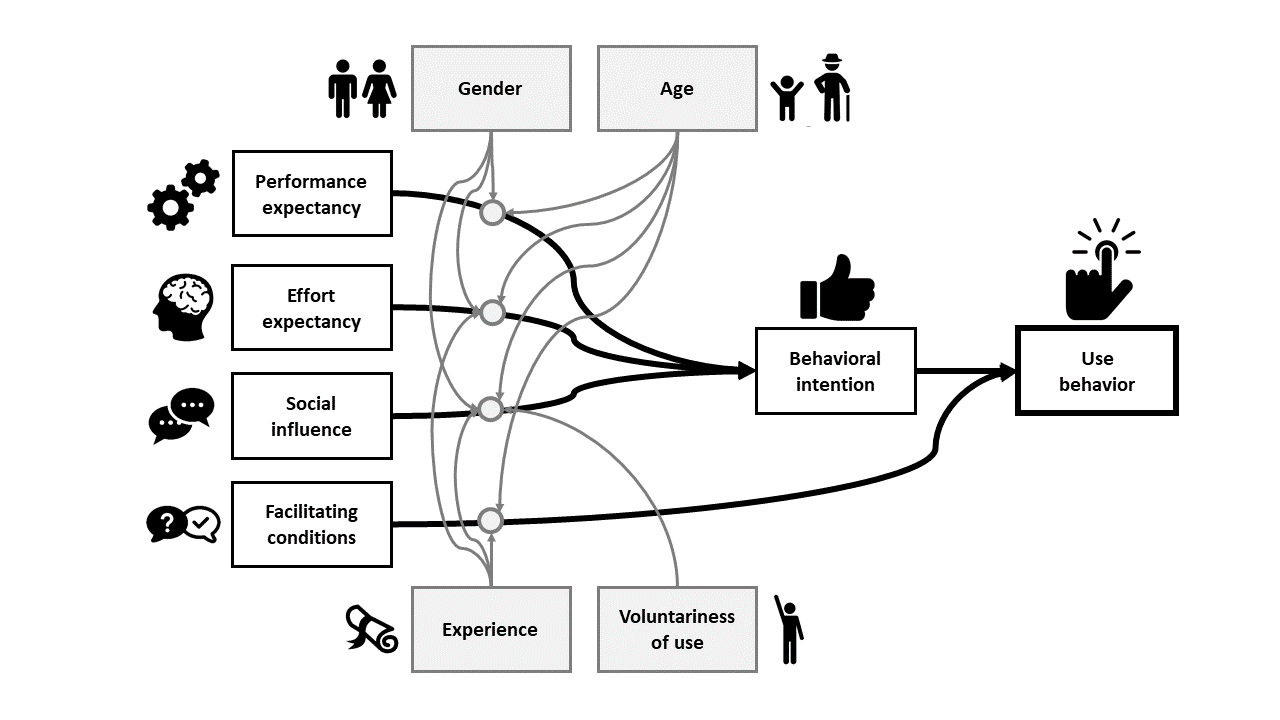
\includegraphics{./media/17-acceptance-of-new-technology-–-the-most-prominent-theories/media/image3.png}
\caption[The variables and moderators in the UTAUT model (Venkatesh et al., 2003) ~]{The variables and moderators in the UTAUT model (Venkatesh et al., 2003)\footnotemark{} ~}\label{fig:figure163}
}
\end{figure}
\footnotetext{Icons from Noun project designed by A. Coquet, S. Singh, M. Polakovic, G. Cresnar, A. Uddin, G. Higgins, J. Pictos, and Corpus delicti.}

Since this model was introduced, it has been used extensively by researchers when trying to explain the acceptance and use of technology. Although the model has been successful, newer research has found that these constructs and moderators are not always applicable to all contexts, and some crucial constructs may be excluded (Dwivedi, Rana, Jeyaraj, Clement, \& Williams, 2019). Many studies have not utilized the moderating factors (Venkatesh et al., 2012); one explanation might be that there may not be any variation in the moderators (Dwivedi et al., 2019). As an example, the organization might have decided that the use of the technology is mandatory, which makes the moderator voluntariness not applicable. Dwivedi and colleagues (2019) further argue that the UTAUT model is missing one important aspect, namely, the individual perspective. Attitudes, an individual's positive or negative feelings about performing the target behaviour, play an important role in accepting technology, as suggested in the TPB model. They found that attitude had a central role in an individual's intention to use the technology and that it also had a direct effect on usage behaviour. Therefore, it is proposed that attitude should be an integral part of the UTAUT model in the future.~

\hypertarget{beers-theory-of-organizational-change}{%
\section*{Beer's theory of organizational change~}\label{beers-theory-of-organizational-change}}
\addcontentsline{toc}{section}{Beer's theory of organizational change~}

Implementing new technology also often means an organizational change. Acceptance of new technology is therefore somewhat linked to the success of the organizational change. Unfortunately, approximately 70\% of initiated changes fail (e.g., Burnes, 2011). It is therefore of great value to have an effective approach for organizational change. A rational approach to change is Beer's theory of organizational change (Beer 1988, read in Hughes, Ginnett, \& Curphy, 2015). This model includes many of the issues raised by other researchers in the field and highlights what is important for leaders in organizations to consider if they want to be successful with their change effort. The model can be used as a road map when wanting to implement an organizational change and as a diagnostic tool to determine what went wrong if an investment failed to meet its promises (Hughes et al., 2015). Beer has proposed a formula for organizational change, as seen in fig.~\ref{fig:figure164}.

\begin{figure}
\hypertarget{fig:figure164}{%
\centering
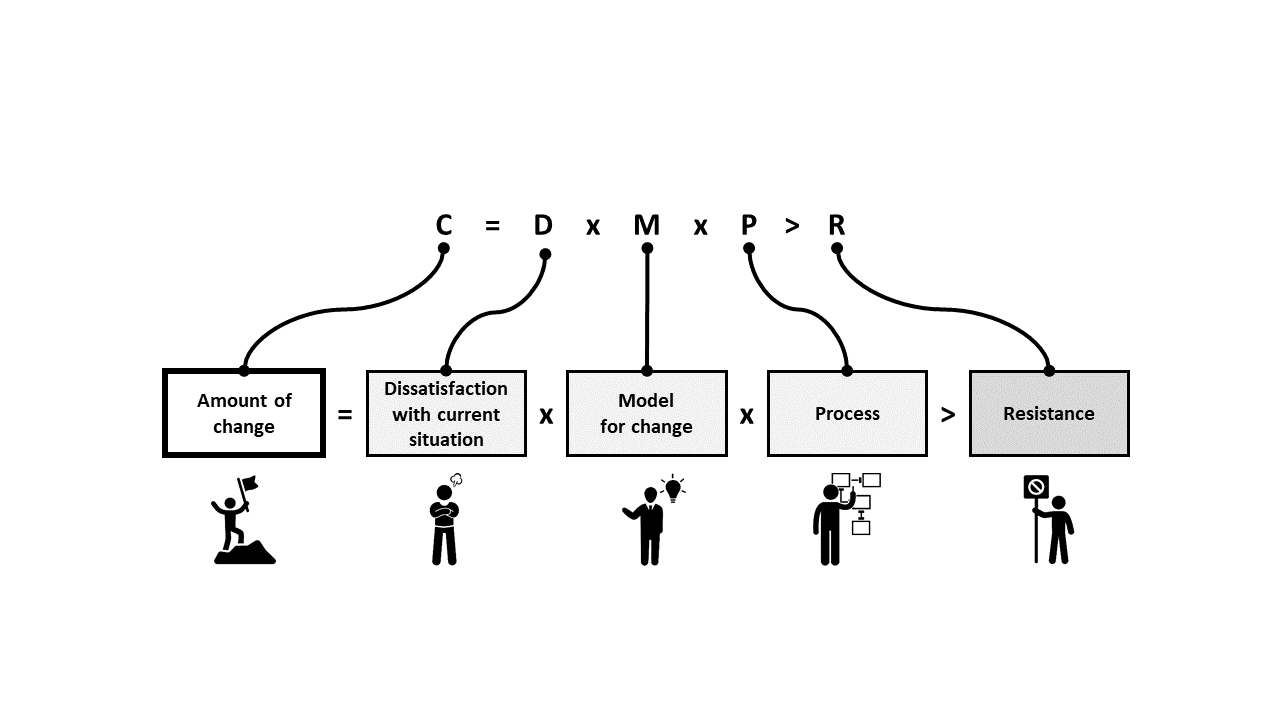
\includegraphics{./media/17-acceptance-of-new-technology-–-the-most-prominent-theories/media/image4.png}
\caption[Beer's (1988, read in Hughes et al., 2015) formula for organizational change]{Beer's (1988, read in Hughes et al., 2015) formula for organizational change\footnotemark{}}\label{fig:figure164}
}
\end{figure}
\footnotetext{Icons from Noun project designed by A. Coquet, G.K. Lay, and M.R. Alam.}

\textbf{\emph{C}} stands for the \textbf{amount of change} that is achieved, and of course ``the more the better''. However, the amount depends on the levels of the other factors in the formula, which needs to be considered to be successful with the change. These factors are briefly described below and exemplified with introducing new technology in a mining context.

The \textbf{\emph{D}} in the formula stands for the employees' \textbf{dissatisfaction} with the current situation. How satisfied the employees are with the current situation is an important factor when trying to accomplish change, because satisfied employees are much less willing to change. In other words, if the employees are satisfied, a key factor for change is to increase dissatisfaction, or stated more positively, to ensure that the employees understand and see the value with the planned change. Let us exemplify: if the organization is about to introduce new technology, then it might be a good idea to first determine how satisfied the employees are with the current situation and/or present technology. If they are satisfied, but the organization nonetheless sees the need for new technology, then it is necessary to stress its importance, which can be done by highlighting economic, competitive, legal, technological and social challenges that the organization faces and what can happen if the change, e.g., dismissal of personnel, bankruptcy, or safety risks, is not implemented (Hughes et al., 2015).~

The \textbf{\emph{M}} stands for the \textbf{model for change}, which primarily constitutes a clear vision for the change and goals that the change is trying to accomplish. The vision should provide guidance for the organization's action, that is, what needs to be changed to fulfil the vision and accomplish the goals (Hughes et al., 2015). To exemplify, the vision could be to be the most attractive mining company in Sweden. To reach that vision, a set of goals needs to be established. One goal can for example be to increase safety. After setting up the goals, which systems need to change to fulfil the vision and accomplish the goals must be decided (Hughes et al., 2015). For example, to reach the goal to increase safety, the organization might decide to implement new technology such as positioning technology. However, to be successful, one needs to think about how changes in one system can affect other parts of the organization (Hughes et al., 2015). For example, if the goal to increase safety includes implementing positioning technology, employees' reaction to that needs to be considered (see Chapter 17). Hence, to increase the odds for a successful change, it is of great value to anticipate possible problems and consider how changes in one system can lead to consequences for other parts of the organization.

The \textbf{\emph{P}} symbolizes the \textbf{process}, which consists of the development and execution of the change plan. A change plan should answer the questions of \emph{what, who, when, where} and \emph{how} the change will happen (Hughes et al., 2015). It might also include planned actions for how to handle possible resistance and how to highlight the importance for change if employees are satisfied with the current situation. A thorough communication plan is also needed, as it is important that all parties are well informed throughout the process. A good way to get the employees committed to the change plan is to let those who are affected by the change be part of creating the plan. Of course, that is not always possible; in that case, it is suggested that commitment to the plan can be increased if the personal benefits of the change are made clear, the expectations are explicitly stated, and there is a trusting relationship between the employees and the leaders (Hughes et al., 2015). In the case of implementing positioning technology, the model suggests that it might be a good idea to let the employees be involved in an early stage to ensure commitment (see also Chapter 17). The resistance may be reduced if they receive a chance to express their fears and suggest solutions, for example on how the information should be handled.

\textbf{\emph{R}} stands for \textbf{resistance}. As already mentioned, people often resist change, which can partly depend on fears of the unknown and of loss. The employees might fear that the change will result in loss of identity, of close relationships with others, of power, or of being seen as competent (Hughes et al., 2015). Resistance can also stem from a temporary drop in performance, which is very common when employees learn new systems and skills. These types of sources for resistance should be taken into account in the change plan. In the case of implementing positioning technology that handles personal information, there might be a fear of violation of privacy and misuse of information (see Chapter 17). One way to handle such fear is to listen to possible concerns and let the employees be part of the change plan.

This model suggests that it is possible for the organization to increase the amount of change by considering different aspects. The level of change can be increased by increasing the level of dissatisfaction with the current situation by communicating the importance and value of the change, presenting a clear vision, developing a well thought-out plan for the change, or by decreasing the employees' level of resistance. However, as seen in fig.~\ref{fig:figure164}, the model is multiplicative, which means that none of the factors can be null if change is about to occur. For example, it does not matter how well thought-out the change plan is or how clear the vision is if there is no dissatisfaction, i.e., the employees are satisfied with the current situation. On the other hand, if there is dissatisfaction with the current situation but there is no plan, then little change will occur. Hence, the model both explains why a change could fail and how to avoid a failure.

\hypertarget{the-importance-of-fairness-justice-and-trust-in-the-workplace}{%
\section*{The importance of fairness, justice and trust in the workplace}\label{the-importance-of-fairness-justice-and-trust-in-the-workplace}}
\addcontentsline{toc}{section}{The importance of fairness, justice and trust in the workplace}

More general psychological concepts that affect emotional and behavioural reactions to the work environment are the perception of fairness, justice and trust in the workplace. The different concepts will be briefly explained below and related to the context of implementing new technology.

\hypertarget{perception-of-justice-and-fairness}{%
\subsection*{Perception of justice and fairness}\label{perception-of-justice-and-fairness}}
\addcontentsline{toc}{subsection}{Perception of justice and fairness}

Humans are highly motivated to strive for justice and have a strong need to feel that they are being treated fairly. These needs are so strong that they have a significant effect in the workplace. Perceptions of justice have been found to affect, for example, job performance, respect for leaders, trust in the organization, thoughts of quitting and tendency to file lawsuits (Conte \& Landy, 2018). There are various types of justice in the workplace; the most frequently discussed are \emph{distributive justice, procedural justice}, and \emph{interactional justice} (see fig.~\ref{fig:figure165}).

Distributive justice, which refers to whether the employees believe they have received (or will receive) fair rewards, are perhaps not that applicable in the context of implementing new technology. However, one example could be if different units receive access to different types of systems; for example, some receive mobile phones while others receive COM radios as communication tools. It should be remembered that distributed justice contributes to the overall perception of the workplace, and employees are found to work harder towards organizational goals if they feel that they are working in a fair and just workplace (Conte \& Landy, 2018). Therefore, acceptance towards using new technology may also be indirectly affected by a general feeling of justice.~

Procedural justice refers to the perception of the fairness of the policies and procedures used in making decisions in the workplace (Greenberg, 1990, read in Alge, 2001). For processes to be perceived as fair, it is important for the employees to feel that they have the opportunity to influence processes and/or outcomes by, for example, being able to express an objection if they believe that the organization has taken an unfavourable action (Conte \& Landy, 2018). It is also important that the employees believe that the organization truly cares and listens to their objections; otherwise, the processes will not produce feelings of justice and fairness. When implementing new technology, it is therefore important to ensure that there is an opportunity for employees to give input into the process and express their hopes and fears. It is equally important for the leaders of a change to show that they genuinely consider the employees' opinions.

Interactional justice refers to how well the employees are treated when procedures are implemented and is suggested to consist of two specific types of interpersonal treatment, namely, \emph{interpersonal justice} and \emph{informational justice} (Colquitt, Conlon, Wesson, Porter \& Ng, 2001). Interpersonal justice reflects the degree to which the employees are treated with politeness, dignity, and respect by the organization. Informational justice focusses instead on the explanations provided to the employees about why procedures were used in that way and hence stresses the need for high-quality communication (Colquitt et al., 2001). When implementing new technology, it is therefore very important to have well-functioning and thorough communication and to give explanations for the change. Equally important is the communication style, which should be warm and supportive.

The feeling of being treated fairly influences a wide range of emotional and behavioural reactions, as mentioned in the beginning of this section. The perception of justice has been found to make the employees accept less-than-perfect working conditions (Conte \& Landy, 2018). On the other hand, the perception of injustice has been proposed to have an even greater impact than justice and can for example lead to retaliation and reduced effort. Once this feeling has arisen, it is extremely difficult to undo the harm. It is therefore important to give thorough information about the process, ensure that the employees can voice their opinions and treat the employees with respect and empathy.

\begin{figure}
\hypertarget{fig:figure165}{%
\centering
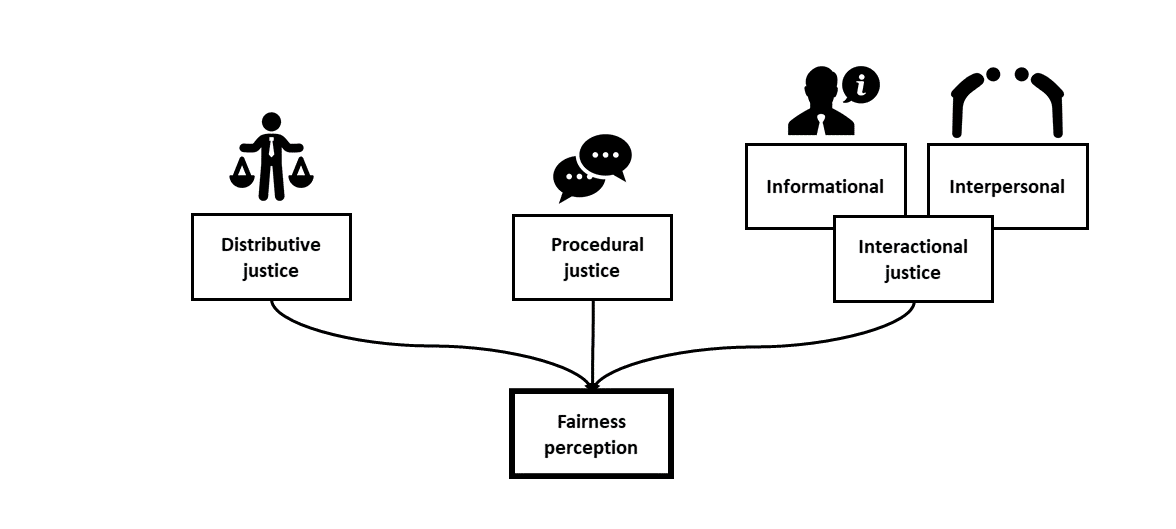
\includegraphics{./media/17-acceptance-of-new-technology-–-the-most-prominent-theories/media/image5.png}
\caption[Types of justice (Conte \& Landy, 2018)]{Types of justice (Conte \& Landy, 2018)\footnotemark{}}\label{fig:figure165}
}
\end{figure}
\footnotetext{Icons from Noun project designed by A. Coquet, D. Kunze, J. Pictos, and S. Wauters.}

\hypertarget{trust}{%
\subsection*{Trust}\label{trust}}
\addcontentsline{toc}{subsection}{Trust}

Many barriers to acceptance of change can be structured under \emph{trust}. Trust is a psychological state, i.e., more an expectation than a reality (Conte \& Landy, 2018). In a broad context, trust means a belief about how a person or an organization will act on some future occasion which is based upon previous interactions with that person or organization (Conte \& Landy, 2018). There are different types of trust. Three types that are relevant in this context are \emph{interpersonal trust}, \emph{organizational trust} and \emph{technological trust} (Montague \& Chiou, 2014, see fig.~\ref{fig:figure166})\emph{.} Interpersonal trust concerns trust between persons, for example, an employer's belief that he or she can trust another person at work, e.g., a colleague (Anderson \& Dedrick, 1990). Organizational trust is the belief that the supervisors and the organization can be trusted (Mayer, Davis, \& Schoorman, 1995). These two types of trust have been found to be especially important when implementing technical systems that collect personal information. To accept such technology, the employees must trust that the people who have access to the information (which can be both colleagues and management) will handle it with care and not misuse the information (see also Chapter 17 for a discussion on this topic). Further, trust in management is a good predictor of lower levels of resistance to change. If the organization lacks, or has lost, the employees' trust, then resistance will be higher, and change will be more difficult to achieve. Technological trust refers to workers' trust in a technology (Timmons, Harrison-Paul, \& Crosbie, 2008). Concerning trust in technology, it is especially important that there is an appropriate level of trust (Montague \& Chiou, 2014). Over-trust or overreliance in the technology and distrust and under-trust can be damaging to work outcomes (fig.~\ref{fig:figure166}). Over-trust in technology can make the workers careless and complacent. For example, the use of positioning technology can make the control room workers rely too heavily on the technology and hence not have a backup plan for a manual rescue operation in case of power failure. On the other hand, distrust among workers, or workers' distrust of technology, may lead to inappropriate or non-use of the technology (Montague \& Chiou, 2014). If workers are required to use technologies that they do not trust, they might create ways to avoid using the technology, which can lead to errors. One such example can be that the workers do not trust the use of the positioning technology and therefore resist wearing the tag and hence remove it, which may lead to devastating consequences in case of a fire or when blasting.

If the newly introduced technology reduces efficiency, decreases safety and is difficult to use, it can negatively impact employee trust in the organization (Montague \& Chiou, 2014). Further, it is found that people who have lost trust begin to seek out information that will confirm their distrust, and they are less open to information that challenges that distrust (Conte \& Landy, 2018). In other words, previously handled implementations can affect how new technology is accepted. Trust is difficult to build but easy to lose (Kramer, 1999). Further, once trust in an organization has been lost, it is extremely hard to rebuild (Conte \& Landy, 2018). Have in mind though, that explanations and apologies can help repair the damage done by violations of trust (Conte \& Landy, 2018), which goes hand in hand with the recommendations to ensure that the workplace is perceived as just and fair.~

\begin{figure}
\hypertarget{fig:figure166}{%
\centering
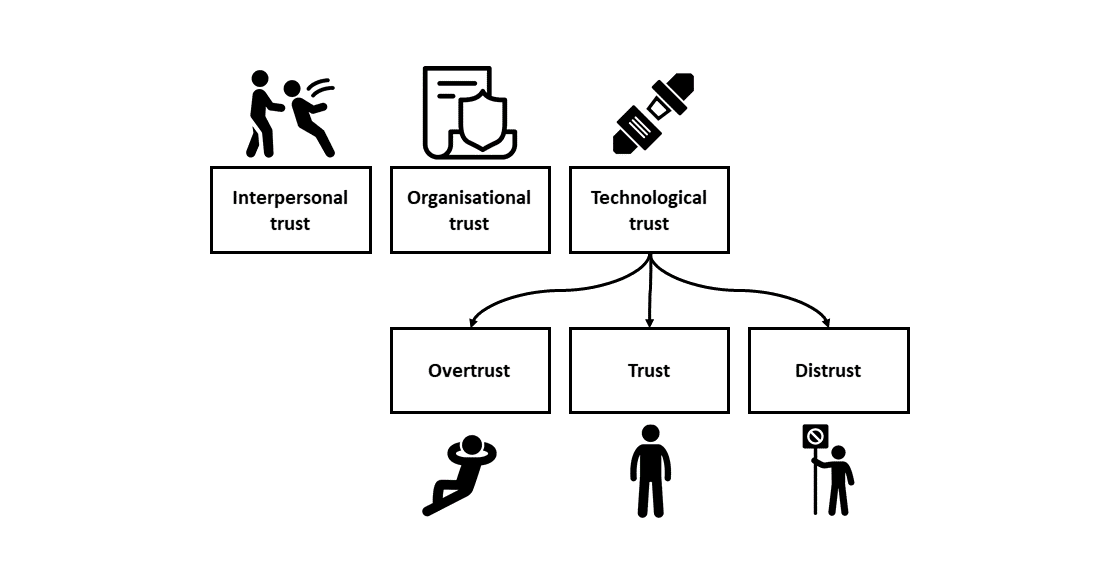
\includegraphics{./media/17-acceptance-of-new-technology-–-the-most-prominent-theories/media/image6.png}
\caption[Different types of trust]{Different types of trust\footnotemark{}}\label{fig:figure166}
}
\end{figure}
\footnotetext{Icons from Noun project designed by A. Coquet, G.K. Lay, Graphic Enginer, and LAFS.}

\hypertarget{positioning-technology-safety-vs-privacy-concerns}{%
\chapter{Positioning technology -- safety vs privacy concerns}\label{positioning-technology-safety-vs-privacy-concerns}}

\begin{chap-auth}
Lisa Öman Ekervhén and Camilla Grane
\end{chap-auth}

This chapter discusses the positive effects of positioning technology from a safety perspective and sets it against privacy concerns. Factors that need to be considered to enhance privacy and reduce the perception of misuse are discussed.

As can be read in chapter 4, a recommendation for creating attractive workplaces in the mining industry is to have health and safety at work as a top priority. This goal can be achieved through mechanization, remote control and automation, and a developed safety climate. An additional means of increasing safety is to use new and advanced communication and positioning technology that works in a mining environment. The communication and positioning technology allows real-time location, tracking and monitoring of vehicles, personnel and equipment. The information can be available both in control rooms on the surface and underground on mobile phones and tablets (see fig.~\ref{fig:figure171}). Such technology entails everyone, wherever they are located, having access to information about what is going on down below (and above ground).~

\begin{figure}
\hypertarget{fig:figure171}{%
\centering
\includegraphics{./media/18-positioning-technology-–-safety-vs-privacy-concerns/media/image1.png}
\caption[Positioning information of objects, people, vehicles and locations can be viewed in mobile phones and on computer screens]{Positioning information of objects, people, vehicles and locations can be viewed in mobile phones and on computer screens\footnotemark{}}\label{fig:figure171}
}
\end{figure}
\footnotetext{Icons from the Noun project designed by A. Coquet.}

From a safety perspective, it is of course a great advantage to see peoples' exact location, for example, in case of a fire or a cave-in that requires evacuation of the mine. In such situations, time is of great importance. Without positioning technology, rescue personnel need to spend much time confirming that each worker is in a safe location. With a positioning system, this phase goes much faster and instead allows the focus to be on those who have not reached safety and supports decisions about who needs attention first.~

Today's technology also makes it possible to collect other types of information from the environment in addition to that from humans. Via sensors, information regarding machine functionality, temperature, tensions, vibrations and similar data can be collected, including information on the surrounding environment such as levels of fumes and gases in the air. A rather new concept is sensors worn by humans, measuring human conditions. Physiological sensors can provide information about \emph{personal health} such as pulse and temperature; biokinetic sensors can measure posture and body movements (\emph{position}); and ambient sensors can measure environmental factors such as temperature or sound pressure level (Johny \& Anpalagan, 2014; fig.~\ref{fig:figure172}). These systems could also be useful as a preventive safety system or in case of an accident, as the information can be shared with other workers close by, control room personnel, and rescue personnel.~

\begin{figure}
\hypertarget{fig:figure172}{%
\centering
\includegraphics{./media/18-positioning-technology-–-safety-vs-privacy-concerns/media/image2.png}
\caption[Information that is possible to collect by positioning technology and wearable sensors]{Information that is possible to collect by positioning technology and wearable sensors\footnotemark{}}\label{fig:figure172}
}
\end{figure}
\footnotetext{~Icons from the Noun project designed by A. Coquet and Ahmad.}

Doubtlessly, this capability is a great advantage, but what do the workers think about such technology? In a safety critical situation, this type of human tracking might be accepted by the workers, but the information could also be misused. As can be read in chapter 15, one must be aware that these kinds of systems are a threat against personal integrity and must therefore be handled with care. According to Zweig and Webster (2002), there is a growing acknowledgement that technologies that track presence and activity lead to privacy concerns. Hence, when implementing such technology, psychological aspects must be taken under consideration.

\hypertarget{important-psychological-aspects-to-consider}{%
\section*{Important psychological aspects to consider}\label{important-psychological-aspects-to-consider}}
\addcontentsline{toc}{section}{Important psychological aspects to consider}

Privacy can be defined as the extent to which individuals believe they have control over their personal information and interactions with others (Stone \& Stone, 1990). The individual perceiving a loss of such control can lead to a perception of invasion of privacy. Privacy concerns are one of the most consistent reactions to awareness systems (e.g., Zweig \& Webster, 2002). Hence, positioning technology and human sensors can lead to the feeling of lost control if not restricted and handled properly. Based on research and findings from the SIMS project and other related projects, we will now briefly exemplify some psychological aspects that are important to consider to avoid violating privacy and to create acceptance for techniques that collect personal data.

One important aspect is that the collected information must be perceived as being \emph{relevant,} i.e., necessary and appropriate to collect. Collected information that is perceived as relevant is more likely to be viewed as less invasive of privacy than information that is perceived as irrelevant (e.g., Alge, 2001). It is therefore extremely important that each bit of information that is collected can be justified on good grounds. Have in mind that, although today's technology makes it possible to collect all sorts of information, information should not be collected only because it is possible to do so. The more the merrier does not apply in this context. For example, if one's position is of importance only from a safety perspective, then it may be of less importance to view the name of the person.~

It is of great importance to make the \emph{usefulness} of the technology visible for the workers to achieve acceptance (e.g., Davis, 1993). The organization must be able to communicate \emph{why} such systems should be implemented. As when children ask ``why'', ``because'' is not a good answer. Are you satisfied with such an answer? Hence, the organization must be able to justify its use, that is, have a legitimate reason for implementing the system. From a privacy perspective, the individual wants to have control over what information the organization has \emph{access} to and how the organization will \emph{use} the collected information (Brandimarte, Acquisti, \& Loewenstein, 2013). Most important for accepting the revealing of personal information is likely to be control over how the information will be used. In this context, be careful to ensure and clarify the purposes for collecting possibly sensitive information and to communicate the true purpose. It is also important to explain the usefulness clearly. For example, ensure that the workers understand how the technology will enhance \emph{their} safety and facilitate rescue operations. A further aspect is to emphasize the accompanying advantages such technology can have for the workers in their everyday job, in terms of being able to locate persons, vehicles and equipment and of providing information about the surrounding environment.~

\emph{Participation} is a key component for enhancing employees' perception of procedural justice and reducing feelings of invasion of privacy (Alge, 2001). It is therefore important to allow employees to be involved in both the design and implementation of the technology. The workers should be involved at an early stage, even if introducing the technology is mandatory, i.e., not optional. They should be included when discussing and deciding \emph{what} information should be collected, \emph{who} will have access to the information, and \emph{how} the information should be stored and handled, etc. For example, knowledge of who is able to monitor you has been found to lower perceptions of privacy invasion (Zweig \& Webster, 2002). One further advantage of including workers early in the process is the possibility of understanding their hopes and fears. It is important to be responsive to any concerns that employees might have and try to sort them out at an early stage. Therefore, the most sceptical employees can be a valuable resource. If their concerns are listened to and met, there is a greater possibility that the technology will be accepted when implemented.~

Our attitudes are influenced by important others, and attitudes towards positioning technology are no exception. In other words, an individual worker's attitude to such technology can be influenced by the attitudes of the colleagues (\emph{social influence}). This point is especially true in mandatory settings, i.e., when using the technology is not optional (e.g., Venkatesh, Morris, Davis, \& Davis, 2003). The influence of others' opinions tends to be highest in the early stages of experience with the technique before the individual has had time to form their own opinion. Each worker's individual \emph{a priori} attitude about the technology cannot simply be summed to predict whether the group will decide to adopt the technology unless they all are in agreement (Sarker, Valacich, \& Sarker, 2005). If not in agreement, a complex group interaction process will start, where they attempt to influence each other, which in turn results in the group adopting or not adopting the technology. This process implies that it is important to view the implementation of new technology as a group process and therefore also handle it on a group level. It is also extremely important to remember that workers also influenced by the management; therefore, managers must communicate support and belief in the system. In other words, acceptance of the technology must permeate the entire organization.

The human strives for the perception of \emph{justice} (see also Chapter 16). Therefore, to achieve acceptance for positioning technology, it may be of importance that everyone can see everyone's position. If a worker is monitored differently than are other co-workers or other professionals, that worker may experience injustice (Alge, 2001). The feeling of big brother's watching you should be avoided. It has also been found that mere suspicion that the information could be used for performance monitoring creates a perception of unfairness (Zweig \& Webster, 2002). Hence, if there is no such intention with the system, it is important to make that clear.

Another important factor that can affect acceptance for technical systems that collect personal information is \emph{trust}. Such systems require a level of trust in the relationships between colleagues, managers and the organization. Trust in this context means the belief that the other party (who collects the data) will behave in a responsible manner and by doing so also fulfil the trusting party's (the employee's) expectations without taking advantage of its vulnerabilities (Pavlou, 2003). Hence, the employees must trust that the people who have access to the information will handle it with care and not misuse it. When interviewing workers who have experience with positioning technology, trust is a frequently mentioned aspect for accepting the technology. A further type of trust is workers' trust in a technology (Montague \& Chiou, 2014). Distrust among workers, or workers' distrust of technology, may lead to inappropriate or non-use of the technology (Montague \& Chiou, 2014). If workers are required to use technologies they do not trust, they might create ways to avoid using the technology, which can lead to errors. For example, if the workers do not trust the use of the positioning technology, they may resist wearing the tag and hence remove it, which can lead to devastating consequences in case of a fire or when blasting.

The implementation of new technology requires \emph{proper training}. Much money is spent on developing new technology, but much less is spent on educating the personnel who will use it on \emph{how} to use the technology. This step is often forgotten. It can be summarized as ``too little training and too late''. As an example, in the event of an accident, it is not desirable for the personnel in the control room to see the emergency functions for the first time. Further, another side of trust besides trust in relationships (see the section above) is over-trust in technology. What happens if the system goes down because of a power failure and the position technology cannot be used? Then, it is important to have a backup plan and have had proper training on how to handle such situations with manual routines.

Humans are generally sceptical about change; there is a fear of the unknown. Change can be perceived as stressful, which leads to negative emotions and feelings of uncertainty that in turn can affect acceptance. This result can be countered with thorough information. Therefore, it is extremely important to keep personnel updated at all stages in the implementation of positioning technology and to ensure that all personnel receive the same information (to create justice).~

There are of course other important aspects to consider, but the purpose of this chapter was to highlight some of the most important psychological aspects that need to be considered when implementing technology that handles personal information. The aspects are summarized in the following bullet list:~

\begin{itemize}
\item
  Ensure that the system only collects relevant information.~
\item
  Ensure that the implementation is justified on good grounds.
\item
  Ensure that the usefulness of the system is visible for the individual workers.
\item
  Make clear what the purpose of the system is and what it is not (e.g., not performance monitoring).
\item
  Design and implement the technology in close cooperation with the workers.
\item
  Consider change a group process (social influence).
\item
  Ensure that acceptance permeates the entire organization.
\item
  Ensure that the technology is used fairly and create guidelines that restrict the use of the system and that include individual rights, how the information will be stored, and who will have access to what information, and so forth.~
\item
  Ensure that trust exists in the organization.
\item
  Ensure that the users receive proper training.
\item
  Give the workers thorough information, and ensure that there are forums to vent questions about expectations and fears with the technology.
\end{itemize}

\hypertarget{investing-in-new-technology-how-to-do-it-right-or-understand-what-went-wrong}{%
\chapter{Investing in new technology: how to do it right or understand what went wrong}\label{investing-in-new-technology-how-to-do-it-right-or-understand-what-went-wrong}}

\begin{chap-auth}
Lisa Öman Ekervhén and Camilla Grane
\end{chap-auth}

This chapter provides guidelines or questions to consider when investing in new technology. These questions are meant to aid the organization in the process of selecting, developing and introducing new technology that is effective, efficient and accepted from a user perspective. The chapter can also be used as a guide in more general development processes. It does not describe the process itself, but it points out some important aspects to consider to achieve high acceptance of a change. The guideline can also be used as a diagnostic tool to determine what went wrong if an investment or change process fails to meet its promises regarding acceptance and use.~

Although the intention (often) is good when introducing new technology in an organization, there is no guarantee that the intended users will accept and use the technology. Further, although the technology is ``right,'' people might not accept it (Zweig \& Webster, 2002). Hence, there are several aspects that need to be considered to gain acceptance and succeed with the implementation. The best means of achieving a successful implementation of new technology is of course to proactively avoid making mistakes that can be thought of beforehand.~

Based on research introduced in previous chapters (see for example Chapters 16,17 and 19) and on our experiences from the SIMS project and other similar projects, we have created a guideline consisting of questions that are good to consider before implementing new technology to attain acceptance. The questions are organized around the different aspects that they are supposed to consider.

\hypertarget{clear-vision}{%
\section*{Clear vision~}\label{clear-vision}}
\addcontentsline{toc}{section}{Clear vision~}

\begin{itemize}
\item
  What is the purpose of implementing the new technology?
\item
  What are the goals with the new technology?
\item
  Are the purpose and goals clear for the employees?
\item
  Can the new technology have consequences for other parts of the organization?
\end{itemize}

Of course, the purpose for implementing new technology should be known and well thought-out; however, a clear vision and intended goals should also be formulated, that is, written down (Beer 1988, read in Hughes, Ginnett, \& Curphy, 2015). The vision and goals must also be communicated to all employees who are affected by the new technology. Hence, the organization must be able to justify and give a legitimate reason for implementing the technology. One also needs to think about how changes in one system can affect other parts of the organization.~

\hypertarget{perceived-usefulness-performance-expectancy}{%
\section*{Perceived usefulness (Performance expectancy)}\label{perceived-usefulness-performance-expectancy}}
\addcontentsline{toc}{section}{Perceived usefulness (Performance expectancy)}

\begin{itemize}
\item
  Will the new technology improve the quality of the work?
\item
  Will the new technology make it easier to accomplish tasks more quickly?
\item
  Will the new technology improve safety at work (or another significant aspect)?
\item
  Overall, is the technology perceived as useful?
\end{itemize}

The purpose for implementing new technology may of course vary; however, it is important to ensure that the workers see the usefulness of the technology to attain acceptance and increase actual use (e.g., Davis, 1993; Venkatesh, Morris, Davis, \& Davis, 2003).~

\hypertarget{perceived-ease-of-use-effort-expectancy}{%
\section*{Perceived ease of use (Effort expectancy)}\label{perceived-ease-of-use-effort-expectancy}}
\addcontentsline{toc}{section}{Perceived ease of use (Effort expectancy)}

\begin{itemize}
\item
  Is the new technology easy to learn and remember how to use?
\item
  Is the new technology easy to understand and interact with?
\item
  Is the new technology flexible and possible to use for all workers?
\item
  Is the new technology easy to use and bring in the contexts in which it will be used?
\item
  Overall, is the new technology perceived as easy to use?
\end{itemize}

However, it is not enough that the users believe the technology to be useful; it will not be accepted unless they also believe the technology to be easy to use (e.g., Davis, 1993; Venkatesh et al., 2003). Consistent with human-centred design (see Chapter 19), it is therefore important that the design of the new technology is based on the needs and wants of the people who interact with it instead of having them accommodate the technology, as it can improve employee acceptance of workplace changes (Horberry, Burgess-Limerick, \& Steiner, 2018). It is also important to consider and test the technology in its right context of use. Consider for example background noise, dirt, work situations, safety equipment and work clothes. For example, if the users are obliged to wear gloves, the technology should be possible to use with gloves.~

\hypertarget{inclusiveness}{%
\section*{Inclusiveness}\label{inclusiveness}}
\addcontentsline{toc}{section}{Inclusiveness}

\begin{itemize}
\item
  Can the new technology be used independent of size and strength?
\item
  Can the new technology be used independent of age?
\item
  Can the new technology be used by non-natives?
\item
  Can the new technology be used by people with disabilities?~
\end{itemize}

As an extension of usefulness, it is extremely important to take into account that people differ and the technology must therefore be inclusive, i.e., well suited for all workers irrespective of gender, age, and height, etc. (see also Chapter 19). Many workers also have common disabilities such as dyslexia or colour blindness that may interfere with their interaction with some systems. Additionally, there may be entrepreneurs or workers hired temporarily that do not speak the native language; it is important to ensure that they could still understand and use the technology and follow safety routines. Hence, ensure that the technique is suitable, comfortable and safe to use for more than just the average person.

\hypertarget{facilitating-conditionsperceived-ability}{%
\section*{Facilitating conditions/Perceived ability}\label{facilitating-conditionsperceived-ability}}
\addcontentsline{toc}{section}{Facilitating conditions/Perceived ability}

\begin{itemize}
\item
  Will the users have the resources necessary to use the system?
\item
  Will the users have the competence/knowledge needed to use the technology?
\item
  Will the users receive appropriate support if they do not know how to use the technology?
\item
  Will the users receive appropriate support if the technology fails to work?
\item
  Is the technology compatible with other technologies or systems used in the workplace?
\end{itemize}

Organizations can spend a great deal of money on developing and implementing new technology, but much less is spent on educating the personnel who will use it. It is therefore important to consider these types of questions at an early stage and to ensure that an organizational and technical infrastructure exists to support the use of the new technology (e.g., Venkatesh et al., 2003).~

\hypertarget{participation}{%
\section*{Participation}\label{participation}}
\addcontentsline{toc}{section}{Participation}

\begin{itemize}
\item
  How can the employees be involved in the decision to implement the new technology?
\item
  How can the employees be involved in the implementation phase?
\end{itemize}

A good approach to convincing the employees to accept changes in the organization is to let those who are affected by the change participate in the process (Hughes et al., 2015). Of course, it is not always possible for the employees to be involved in the decision, although they might be able to influence certain aspects within given frames. Employee representatives, for example the union, should also be~part of the decision process. Employees could more easily be part of the implementation phase. For example, they could be part of writing instructions or decide on use strategies.

\hypertarget{social-influence}{%
\section*{Social influence~}\label{social-influence}}
\addcontentsline{toc}{section}{Social influence~}

\begin{itemize}
\item
  Are the employees positive towards using new technology?
\item
  Are the employees positive towards changes at work?
\item
  Is the implementation supported by the managers in the organization?
\end{itemize}

The opinions of colleagues, managers, supervisors, family and friends are important when an individual user is forming an intention to use new technology. This point is especially true in mandatory settings, i.e., when using the technology is not optional (e.g., Venkatesh et al., 2003). The influence of others' opinions tends to be highest in the early stages of experience with the technology before the individual has had time to form their own opinion. Additionally, workers are influenced by the management; therefore, managers must communicate support and believe in the system. In other words, acceptance of the technology must permeate the entire organization.

\hypertarget{implementation-plan}{%
\section*{Implementation plan}\label{implementation-plan}}
\addcontentsline{toc}{section}{Implementation plan}

\begin{itemize}
\item
  Is there a clear plan that clarifies \emph{who, what, when, where} and \emph{how} the implementation of the technology should take place?
\item
  Is the plan communicated to everyone in the organization?
\end{itemize}

A thorough plan increases the chances of a successful implementation. The plan should for example include timelines, key deliverables, and a description of who is responsible for what (Hughes et al., 2015). Because employees who are satisfied with the current situation are less willing to change, and because people often resist change, it might be a good idea to also include planned actions for how to handle possible resistance and increase dissatisfaction. It is important to ensure that the employees understand and see the value of the planned change. It is also important to ensure that the plan is clearly communicated to all affected parties in the organization.~

\hypertarget{perceived-justice-and-fairness}{%
\section*{Perceived justice and fairness}\label{perceived-justice-and-fairness}}
\addcontentsline{toc}{section}{Perceived justice and fairness}

\begin{itemize}
\item
  Are new technologies evenly distributed to all employees?
\item
  Can an uneven distribution be justified?
\item
  Are the procedures and outcomes thoroughly expressed and justified?
\item
  Is it possible for the employees to influence the process and/or the outcome?
\item
  Is it possible for the employees to raise concerns about the new technology?
\item
  Are possible concerns considered and taken into account?~
\item
  Are the employees treated with respect throughout the process?
\end{itemize}

The feeling of being treated fairly influences a wide range of emotional and behavioural reactions in the workplace (see Chapter 16). For the workplace to be perceived as fair and just, which enhances acceptance, it is of great importance to give thorough information about the process, ensure that the employees can voice their opinions and treat the employees with respect and empathy (e.g., Conte \& Landy, 2018).

\hypertarget{trust-1}{%
\section*{Trust}\label{trust-1}}
\addcontentsline{toc}{section}{Trust}

\begin{itemize}
\item
  Is there an appropriate level of trust between colleagues?
\item
  Is there an appropriate level of trust in the management?
\item
  Is there an appropriate level of trust in the technology?
\item
  Could the new technology be misused and hence violate trust?
\item
  Is there a risk of over-trust or distrust, and how will this risk be addressed?
\end{itemize}

Many barriers to acceptance of change can be structured under trust. Trust in management is a good predictor of lower levels of resistance to change. If the organization lacks, or has lost, the employees' trust, then resistance will be higher, and change will be more difficult to achieve. A further type of trust is workers' trust in a technology. However, it is important that there is an appropriate level of trust, as over-trust or overreliance and distrust and under-trust can be damaging to work outcomes (Montague \& Chiou, 2014). Over-trust can make the workers careless and complacent, while distrust among workers, or workers' distrust of technology, may lead to inappropriate or non-use of the technology (Montague \& Chiou, 2014). It should be remembered that trust is difficult to build but easy to lose (Kramer, 1999).~

\hypertarget{privacy-concerns-intrusiveness}{%
\section*{Privacy concerns (Intrusiveness)}\label{privacy-concerns-intrusiveness}}
\addcontentsline{toc}{section}{Privacy concerns (Intrusiveness)}

\begin{itemize}
\item
  Is there any risk that the new technology or information that it collects can be perceived as intrusive?
\item
  Is there any risk that the new technology or information that it collects can be misused?
\item
  How can the data be restricted in terms of what to collect?
\item
  How can accessibility be limited in terms of who has access and when data can be accessed? There are at least two alternatives to consider:

  \begin{itemize}
  \item
    Access to data is restricted; for example, data are only accessible to the crisis management group in emergencies.
  \item
    Data are open and accessible for all employees.~
  \end{itemize}
\end{itemize}

Privacy can be a concern if individuals believe they do not have control over their personal information and their interactions with others (Stone \& Stone, 1990). The individual perceiving such a loss of control can lead to a perception of invasion of privacy. Today, there is an increase in what data can be collected that may be perceived as private, for example, your current position, your conversations, your arousal level, your drowsiness, and even your facial expressions. New technologies challenge personal boundaries. Based on Davis' (1993) model, we could assume that acceptance towards new privacy-violating technologies will be low if the usefulness is not clear. Trust should also be considered. It is recommended that the use of information is strictly limited to its purpose and not used for other purposes. Employees will sooner or later discover whether the technology is used as a tool for increased management control and supervision, and their trust will be violated if that use is not coherent with the communicated intended use.~

\hypertarget{adapting-the-technology-to-the-miners-human-factors}{%
\chapter{Adapting the technology to the miners' human factors}\label{adapting-the-technology-to-the-miners-human-factors}}

\begin{chap-auth}
Erik Sundström
\end{chap-auth}

Human-centred design, commonly interchanged with the term human factors design, is defined by Horberry, Burgess-Limerick, \& Steiner (2018) as the science of designing equipment, workplaces, tasks and organizations to account for the users' needs and wants. In other words, designers need to ensure that they accommodate a wide range of users of different shapes, sizes, genders, ages and more. This definition also entails considering the effects that the design has on other stakeholders, such as on maintenance workers who repair the equipment.

The goal of human-centred design, or HCD, is to improve work performance and the safety, health and well-being of the workforce (and, if possible, society at large). According to Horberry m.fl. (2018), the key principles for HCD can be summarized as follows:

\begin{enumerate}
\def\labelenumi{\arabic{enumi}.}
\item
  Adapt the equipment, system or product to the needs and wants of the people who interact with it instead of having them accommodate the system or object. For example, controls and equipment should be designed to be easy to use and perform maintenance on. People should not have to work with the equipment or system in unhealthy or dangerous ways to make it function properly.
\item
  Designing systems or equipment requires an understanding of the people who will interact with or be affected by it. Questions such as what the context for their interaction is, what tasks do they need to perform, in what environment and so forth need to be investigated are asked.
\item
  Continuous involvement of the users and other stakeholders in the design and development process is important to ensure that the previous principles can be upheld.
\item
  The design process is iterative to ensure ideas and concepts are reworked until they fulfil established requirements. Amongst these requirements are needs to account for human-centred subjects such as usability, safety and ergonomics.
\item
  Each stage of the design process of the equipment or system must accommodate the needs and wants of the people who will be interacting with it.
\end{enumerate}

There are several potential benefits with designing in accordance with human factors:

\begin{itemize}
\item
  May allow for solutions or performance improvements not otherwise possible.
\item
  Improves operator performance and efficiency and lowers costs of training.
\item
  Can help avoid additional costs and problems stemming from equipment, workplaces or tasks being badly adapted to the users.
\item
  Demonstrates that the company accommodates their employees' needs and wants. This benefit can improve the attractiveness of the workplace and the products for potential employees and customers.
\item
  Can improve employee acceptance of workplace aspects, changes and tasks.
\item
  Can increase trust from the people involved in the human factors-designed system.
\end{itemize}

According to Horberry, Burgess-Limerick, \& Steiner (2011), human factors are rarely considered when designing mining equipment. Instead, focus often lies on what the technical aspects of the equipment can achieve. The people are often left to perform the tasks that the machines cannot. This doesn't mean that there aren't parts of the mining workplace where human-centred design is currently being taken into account. Below are~some~examples of areas of mining workplaces where human-centred design~is or should be designed for.

The vehicles and machines used in mining have, according to Simpson, Horberry, \& Joy (2009), had problems with cabin visibility for a long time. Due to the size and equipment of the vehicles, the drivers' line of sight is often very limited. The risks and potential consequences of this problem have inspired the implementation or design of several preventative measures, including added cameras to show the ``blind spots'' of the driver's line of sight, proximity sensors to notify the driver on how close they are to things in their environment and more.

The interfaces of mining equipment and machines often contain many buttons, levers and other interactable elements. A human-centred design ensures, amongst other things, that no parts of the interface are difficult or unergonomic to reach. The most-commonly used levers and buttons are the easiest to access. Furthermore, interactable elements need to be grouped up on the interface according to function, for example by placing buttons next to the dials and screens that they interact with.

Relating to unergonomic interfaces, foot rests, seats, handles and other physical elements of the machines can easily become uncomfortable or even perilous to use if they are not designed to accommodate people of different sizes and statures. Tools and equipment can have the same problem, where their weight and size do not consider the physical capabilities of different users. To design with a human-centred focus is to ensure that equipment, tools and other elements in the workplace are comfortable and safe to use for more than just the average person. Making the equipment modifiable and adaptable, such as chairs that can be adjusted and helmets that can fit more people, helps ensure that all employees can safely and effectively use it. It is not enough, however, to ensure that the equipment is comfortable and safe for the users to work with. The equipment also needs to be designed with maintenance in mind. Maintenance hatches, engine housings and electronics need to be reasonably easy to access to not complicate maintenance work more than necessary. Concerning future technologies in mining, the batteries of the electrical vehicles that are to be implemented in the mines need to be easily charged and replaced. Designing and creating these future technologies provides an excellent opportunity to create machines, systems and equipment that accommodate the users and the people affected by such elements.

There are aspects of the future vision for mining workplaces that resemble human-centred design thinking. Mining industries are moving towards utilizing more remote-controlled machines and control room work in mines. The mining operators can thus be removed from potentially dangerous or ergonomically unhealthy work tasks and environments. This approach reduces their exposure to vibration, dust, blasting gases and the risk of cave-ins, improving the safety and health conditions of the workplace. With future mining workplaces consisting of more remote-controlled work, however, operators will spend more time doing static work in control rooms. The Swedish administrative authority Arbetsmiljöverket (2011) warns of the potential health risks such as circulatory problems caused by too much static work. A workplace with a human-centred design should thus provide its operators with work tasks balanced between physical and static work.

\hypertarget{iterative-design-of-mining-workplaces}{%
\chapter{Iterative design of mining workplaces}\label{iterative-design-of-mining-workplaces}}

\begin{chap-auth}
Erik Sundström
\end{chap-auth}

When making and implementing changes to mining industries, it is rare to see large extensive changes take place, which is likely due to the complexities of the systems involved in a mine. Instead, changes are often implemented incrementally, with individual implementations coming together as a larger change effort over a longer period. The development and implementation of changes and solutions can occasionally take between 7 and 10 years to complete, after which they remain in use for at least as long. The problem is that the changes may have already become obsolete at the point of their implementation due to this long implementation process. The designers and planners must thus ensure that they do not introduce long-lasting changes that negatively affect the working environment. This approach can, however, become difficult due to how mining change projects are structured.

According to Lööw, Johansson, Andersson, and Johansson (2019), design processes in mining industries are rarely iterative and human-centred processes, instead following more-linear processes with a technology-centred perspective. While these processes have been successful at times in the mining industry,~there are times where the most relevant issues are only revealed late in the project. A linear process does not allow for earlier parts of the process to be easily revisited, which could make necessary adjustments difficult or expensive. With how long the development times can be for mining implementations, this linear process can risk invalidating several years' worth of work. An iterative design process is more suited for adapting to changing goals and requirements, in addition to placing a greater focus on user feedback. This focus, in turn, provides better opportunities to create results that address relevant issues and user needs.

The iterative design process has been described by several different authors as consisting of a varying number of steps. The process can be generalized, however, into four steps: planning, diagnosis of the present status, formulating demands, and creation and evaluation of proposals. When working with an iterative process, these four steps are followed in order, with more focus being placed on the first steps early in the project. Once all steps have been completed, the process cycles back to the planning phase and work begins again, only this time, more emphasis and detail is placed on the following steps. Osvalder, Rose, Karlsson, Eklund, \& Odenrick (2015) describe this design process using a project circle similar to that shown in fig.~\ref{fig:figure201}. During the cycles, several different solutions should be created to compare and judge between different alternatives. The solutions that satisfy the demands of the project can then be assessed and combined with other solutions, while the solutions that do not can be removed. This design process continues, with each cycle shifting the work focus more towards the final steps, until a final proposal has been gradually developed and chosen.

\begin{figure}
\hypertarget{fig:figure201}{%
\centering
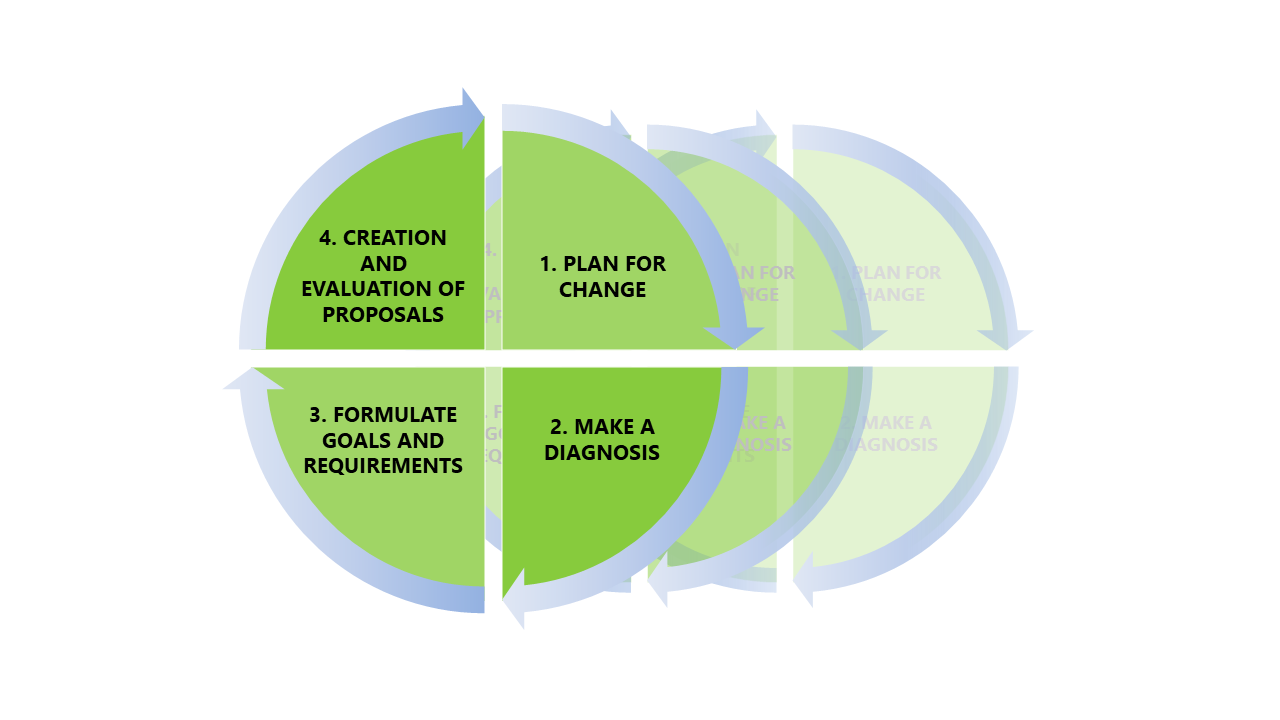
\includegraphics{./media/21-iterative-design-of-mining-workplaces/media/image1.png}
\caption{An illustration of the project circle describing an iterative design process TEMP}\label{fig:figure201}
}
\end{figure}

To more specifically describe the work that goes into the steps of an iterative work process, Ranhagen (1989) starts with describing how the planning phase can be separated into three parts; formulating the goals in general terms, creating a project organization, and separating the work into stages. A project organization can consist of a decision-making body, a health and safety reference group and a project group. The important thing here is to include both people with experience in design work and people from the areas of the workplace who will be affected by the changes, such as maintenance workers or miners. The second step of the iterative process, the diagnosis step, consists of documenting and investigating the current state of the workplace: what problems exist, how the work is done today, what will be done in the future, and so on. In the third step, functional demands are to be established and developed. These demands help guide the creation of concepts and solutions by serving as objectives that need to be fulfilled. At the same time, they need to promote creativity by not specifying a certain solution, for example by having a demand for good air quality instead of a demand for extensive ventilation systems. If one demand is more important than another, a weight point can be applied to each demand that signifies its importance. The final, fourth step entails using different creative methods to create solutions that can then be evaluated based on how well they fulfil the established demands. Here, the weight of the demands can be combined with how well the solution fulfils them to create a score system, allowing the designers to see which solution generally best fulfils the demands. It is important to note, however, that having the highest score does not guarantee that the solution is the best choice. Before deciding, the results should be assessed to see whether the solution is sensible or whether another solution is a viable alternative despite not scoring as high.

As mentioned previously, the benefits of using iterative design processes in mining industries comes from the flexibility in creating solutions. This flexibility helps make projects less vulnerable to changes in focus or to a new problem arising midway through. Furthermore, an iterative process offers more opportunities to create attractive workplaces for both new and existing employees by involving them more in the design process, making it easier to discover and adapt the solutions to their needs and wants, which helps create workplaces where they want to work.

\hypertarget{more-research-is-needed}{%
\chapter{More research is needed}\label{more-research-is-needed}}

\begin{chap-auth}
Jan Johansson and Lena Abrahamsson
\end{chap-auth}

Future efficient mining operations will be dependent upon a highly competent and well-motivated work force on all levels. The mining companies will have to recruit their personnel from a limited group of talented individuals with high demands and expectations of future work. To cope with the future labour supply, the mining industry must change the image of mining work and increase the attractiveness of working in the sector, especially for young women and men.

We know a great deal about what creates an attractive job, but we do not know everything. It is important that the mining industry keeps up with this quest for knowledge; the world is changing, and new knowledge is required. The winners are those who apply the knowledge quickly and translate it into practice.

Below, we describe several activities required to attract and keep skilled personnel in the future mining industry. To achieve this goal, we have identified six areas that need further clarification through research:

\begin{itemize}
\item
  Digitalization opens up new opportunities to create attractive workplaces in a safe environment and jobs that provide space for the employee's full expertise and creativity. However, there are also risks that need to be addressed, such as privacy issues, increased stress and work-life boundaries.
\item
  With the increased digitization, new qualifications are needed. These must be identified, and programmes for reskilling and lifelong learning must be formed.
\item
  Research on health and safety has been successful, but the industry still needs innovative methods to control health and safety-related issues. To be perceived as a safe industry, a zero vision is required based on better proactive safety work.
\item
  Health and safety conditions for contractors must be explored, and more-inclusive safety cultures must be developed.
\item
  Companies must be proactive and try to avoid creating problems in the first place. This result is especially important in mining, where initial mistakes can have consequences for a very long time.
\item
  Finally, it is necessary to develop a holistic concept for the attractive mine that can attract young people.
\end{itemize}

Research must work with these issues from different time perspectives. The long-term vision is the zero-entry mine where all machines are self-regulated or remote-controlled from operation centres above ground. These centres are designed to promote cooperation and creative problem solving in multiskilled teams of men and women. Basic safety level is not an issue anymore; dangerous work tasks are performed by robots.

From a shorter perspective, many workers remain underground. Here, there are new methods for iterative mine planning that take work environment and safety into account and reduce common initial design errors when mines are planned. Production is organized through a holistic approach based on production teams and broad professional skills among management and miners; mining work has been transformed into being attractive to both women and men, not only because of the wages but also because it is an interesting occupation with good potential for personal and professional development and lifelong learning in a safe and sound working environment. Nonetheless, several issues of attractive workplaces should also be considered in future research and innovation; the most important are addressed below.

First, digitization and its effects have an obvious place in a future research agenda. Used correctly, digitalization can create attractive jobs that provide space for the employee's full expertise and creativity. However, there are also risks that need to be analysed and considered. Furthermore, competence development and learning at work, etc., should be prioritized. These topics are vital to meet the demands of new technology and can guarantee flexibility for the company and development in one's professional role. Important focus areas for research are the following:

\begin{itemize}
\item
  How can the new roles of the operators (i.e., ``Operator 4.0'') meet the values and expectations that young women and men have when they enter work life?
\item
  How should digitized production systems address privacy issues?
\item
  How can employers gain acceptance of and avoid resistance to new technology?
\end{itemize}

There is a need for new methods for learning at work, something both employers and employees want. To guarantee development in one's professional role and inhibit becoming stuck in the demands of a special task requires a certain degree of generalness in competence development. Broad work roles are a classic demand that can also be combined with the ideas behind lean mining. The industry has a general need to recruit more women. Important focus areas for research are the following:

\begin{itemize}
\item
  Identification of future skills requirements
\item
  Development of new education programmes for reskilling and competence development of management and workers as part of lifelong learning
\item
  Develop a strategy for recruiting more women
\item
  Develop a mentor system for miners so that professional knowledge is transferred between generations
\item
  Develop VR and AR for training and simulation, particularly for operations in hazardous environments
\end{itemize}

Health and safety at work must have top priority. Mechanization, remote control and automation are efficient preventive safety measures. They are also appropriate for reducing workload to avoid musculoskeletal injuries and allow for recovery periods. New technology makes it possible to both warn of dangerous working conditions and monitor employees' health conditions in real time. Improved safety is also a matter of a developed safety climate in the form of relevant education, rules and effective leadership, with safety prioritized in the day-to-day work. In short, there is a need for further development of the following:

\begin{itemize}
\item
  How we can increase safety by monitoring the operators in real time?
\item
  New methods for monitoring and controlling the work environment
\item
  Efficient tools for proactive safety control, and broader analyses of the impact of digitalization on health and safety in general
\item
  Upgraded safety climate
\end{itemize}

Moreover, the increased number of contractors must be addressed. The focus should be on the benefits and potential problems that come from a workforce of in-house personnel and contractors. This focus includes strengthening both formal (e.g., implementing joint safety management practices) and informal (e.g., communication and interaction in the workplace) relations at multiemployer worksites. Important issues in this area include the following:

\begin{itemize}
\item
  Reviews of the health and safety conditions for contractors in mining
\item
  The development of a safety culture that includes contractors
\end{itemize}

Many problems in the work environment in present mines (and in other industries) can be traced back to insufficient initial physical planning and design. Since mining is characterized by huge investments and long-term operations, it is very important that it is based on a well-designed physical production system. The physical layout also influences and limits the organizational aspects. If initial mistakes are made, personnel will have to withstand the negative consequences for many years to come. The initial design phases of every major development project are therefore critical for establishing a safe and attractive physical and psychosocial work environment in a mine.

The main idea and research task in this challenge is to combine and further develop a general iterative industrial planning and design method (Ranhagen, 1995) with available and relevant work environment tools and combine them with the demands of the new technology. The final product, which is planning guidelines with a focus on work environment design in underground mines, should be adapted to the users' (pre-study engineers, feasibility engineers, project planners, automation engineers, layout planners, and ventilation planners, etc.) needs and professional situation. Such guidelines, preferably integrated with CAD planning and design tools, would help these professionals to create safer and more attractive future workplaces in the mines.

Designers of mine productions systems also have many legislative and compulsory provisions to follow and company-specific rules and standards for the work environment and the management of health and safety (Johansson and Johansson, 2008). These aspects must also be integrated into the guidelines for work environment planning and design. The major research task can be described as follows:

\begin{itemize}
\tightlist
\item
  Development of alternative guidelines for early and critical stages of future mine design
\end{itemize}

Finally, although the traditional image of mining is not particularly attractive, and the industry still has health and safety issues that need to be considered, we think that it is possible to create a new vision of future mining, i.e., a vision of a high-technology industry that speaks to today's young people. Mining companies must more actively demonstrate their social responsibility. Employees want to feel proud to work in the company, which means that issues such as vision, mission and core values are important. If we manage these problems well, they can be turned into advantages that create new, attractive job roles. All these factors affect the company's image and thus the possibility of recruiting young, talented people to the industry. Overall, broader strategic research areas should include matters related to

\begin{itemize}
\item
  The development of a holistic concept for the zero entry mine;
\item
  The development of efficient programmes for development of attractive societies;
\item
  The development of a model for an ethical, ecological and diverse workplace and recognized as a green branch; and
\item
  Giving the industry a new image that can attract young people.
\end{itemize}

The mining industry must be prepared to meet technological development on human terms. From a longer perspective, this preparedness can lead to a recognition of the mining industry as an ethical, ecological and diverse industry that can offer challenging jobs and attractive workplaces.

\hypertarget{checklist-for-safe-and-attractive-mining-workplaces}{%
\chapter{Checklist for safe and attractive mining workplaces}\label{checklist-for-safe-and-attractive-mining-workplaces}}

\begin{chap-auth}
Erik Sundström
\end{chap-auth}

While ensuring and creating safe and attractive mining workplaces is important, it is understandably not a simple task.
There are many aspects, issues and questions that must be considered and addressed to achieve that goal, enough that it would be very difficult to try and address them all at once. Making wider, simpler analyses on the current state of a mining workplace, however, can still be useful. Identifying what areas of a mining workplace that can be changed to improve safety and attractiveness should be done to allow for early analysis and planning of actions. It is possible, however, that people become blind to the faults and needs for improvement in their working environment. This checklist aims to help highlight potential areas of improvement in a mining workplace that could make it a safer and more attractive workplace, without presenting in-depth solutions that may limit the decisionmaking process.

\hypertarget{key-categories-for-documentation}{%
\section*{Key categories for documentation}\label{key-categories-for-documentation}}
\addcontentsline{toc}{section}{Key categories for documentation}

\begin{itemize}
\item
  Name and/or location of the mine:

  \begin{center}\rule{0.5\linewidth}{0.5pt}\end{center}
\item
  Date of investigation:

  \begin{center}\rule{0.5\linewidth}{0.5pt}\end{center}
\end{itemize}

\hypertarget{safety-and-risks-general-questions}{%
\section*{Safety and risks: General questions}\label{safety-and-risks-general-questions}}
\addcontentsline{toc}{section}{Safety and risks: General questions}

\begin{itemize}
\item
  Are there systems for documentation of incidents, risks and accidents available?

  \begin{itemize}
  \item[$\square$]
    Yes
  \item[$\square$]
    No
  \item
    Are the employees motivated and encouraged to document and report incidents, risks and accidents?

    \begin{itemize}
    \tightlist
    \item[$\square$]
      Yes
    \item[$\square$]
      No
    \end{itemize}
  \item
    Are reports anonymous?

    \begin{itemize}
    \tightlist
    \item[$\square$]
      Yes
    \item[$\square$]
      No
    \end{itemize}
  \item
    Are managers and the organization accepting and welcoming of these reports?

    \emph{(i.e., taking suggestions and warnings to heart, not becoming defensive and/or accusatory towards the one reporting)}

    \begin{itemize}
    \tightlist
    \item[$\square$]
      Yes
    \item[$\square$]
      No
    \end{itemize}
  \end{itemize}
\item
  Are reports of incidents, risks and accidents taken seriously by management?

  \begin{itemize}
  \item[$\square$]
    Yes
  \item[$\square$]
    No
  \item
    Are reports of incidents and risks investigated?

    \begin{itemize}
    \tightlist
    \item[$\square$]
      Yes
    \item[$\square$]
      No
    \end{itemize}
  \item
    Are reports of accidents followed up?

    \begin{itemize}
    \tightlist
    \item[$\square$]
      Yes
    \item[$\square$]
      No
    \end{itemize}
  \end{itemize}
\item
  Are contractors motivated and encouraged to document and report incidents, risks and accidents to the organization?

  \begin{itemize}
  \item[$\square$]
    Yes
  \item[$\square$]
    No
  \item
    Are actions taken to address dangers and risks in contractor workplaces?

    \begin{itemize}
    \tightlist
    \item[$\square$]
      Yes
    \item[$\square$]
      No
    \end{itemize}
  \end{itemize}
\item
  How are hazards most-commonly handled?

  \begin{itemize}
  \tightlist
  \item[$\square$]
    Hazards are eliminated by replacing them in the planning stages.
  \item[$\square$]
    Hazards are isolated so that they cannot reach individuals.
  \item[$\square$]
    Change how people work to reduce the effects and/or risks of hazards.
  \item[$\square$]
    Hazards are encapsulated and limited through enclosures and physical protection.
  \item[$\square$]
    People are isolated from the hazard zone through enclosures and physical protection around the individuals.
  \item[$\square$]
    Risks are reduced through information and training on safe handling of and work with the hazard.
  \item[$\square$]
    The effects of hazards on workers are mitigated with personal protective equipment.
  \end{itemize}
\item
  Are efforts being taken to move towards the higher levels of hazard control?

  \begin{itemize}
  \tightlist
  \item[$\square$]
    Yes
  \item[$\square$]
    No
  \end{itemize}
\item
  Is systematic safety work management practised?

  \emph{(i.e., systematic review of reports, analysis of risks and accidents, and maintaining good safety practices, etc.})

  \begin{itemize}
  \tightlist
  \item[$\square$]
    Yes
  \item[$\square$]
    No
  \end{itemize}
\end{itemize}

\hypertarget{safety-and-risks-mining-specific-questions}{%
\section*{Safety and risks: Mining-specific questions}\label{safety-and-risks-mining-specific-questions}}
\addcontentsline{toc}{section}{Safety and risks: Mining-specific questions}

\begin{itemize}
\item
  Are remote-controlled vehicles used in the mine?

  \begin{itemize}
  \tightlist
  \item[$\square$]
    Yes
  \item[$\square$]
    No
  \end{itemize}
\item
  Are there work tasks where the miners work alone?

  \begin{itemize}
  \tightlist
  \item[$\square$]
    Yes
  \item[$\square$]
    No
  \end{itemize}
\item
  Do the employees take training courses in mine safety?

  \begin{itemize}
  \item[$\square$]
    Yes
  \item[$\square$]
    No
  \item
    Is this training mandatory?

    \begin{itemize}
    \tightlist
    \item[$\square$]
      Yes
    \item[$\square$]
      No
    \end{itemize}
  \item
    Is the training recurring?

    \begin{itemize}
    \tightlist
    \item[$\square$]
      Yes
    \item[$\square$]
      No
    \end{itemize}
  \item
    Do the employees receive additional training if/when changes are made in the workplace?

    \begin{itemize}
    \tightlist
    \item[$\square$]
      Yes
    \item[$\square$]
      No
    \end{itemize}
  \end{itemize}
\item
  Are the presences of the people in the mine registered?

  \emph{(i.e., checking in/out when entering/exiting the mine in case of an accident/if the mine needs evacuating)}
\item[$\square$]
  Yes
\item[$\square$]
  No
\item
  Are employees educated in evacuation procedures in case of an accident?

  \begin{itemize}
  \tightlist
  \item[$\square$]
    Yes
  \item[$\square$]
    No
  \end{itemize}
\item
  Are contractors educated in evacuation procedures in case of an accident?

  \begin{itemize}
  \tightlist
  \item[$\square$]
    Yes
  \item[$\square$]
    No
  \end{itemize}
\item
  Who is evacuated during blasting?

  \begin{itemize}
  \tightlist
  \item[$\square$]
    Everyone in the mine
  \item[$\square$]
    People near the blasting zone
  \end{itemize}
\end{itemize}

Are there procedures for searching for duds after blasting?

\begin{itemize}
\tightlist
\item[$\square$]
  Yes
\item[$\square$]
  No
\end{itemize}

\hypertarget{safety-and-risks-equipment-and-vehicles}{%
\section*{Safety and risks: Equipment and vehicles}\label{safety-and-risks-equipment-and-vehicles}}
\addcontentsline{toc}{section}{Safety and risks: Equipment and vehicles}

\begin{itemize}
\item
  Is standard safety equipment available to the miners?

  \begin{itemize}
  \tightlist
  \item[$\square$]
    Helmet
  \item[$\square$]
    Hi-vis clothing
  \item[$\square$]
    Ear protection
  \item[$\square$]
    Eye protection
  \item[$\square$]
    Work gloves
  \item[$\square$]
    Work boots
  \item[$\square$]
    Breathing mask
  \item[$\square$]
    Lamp/Light
  \end{itemize}
\item
  Do all employees wear/utilize the safety equipment?

  \begin{itemize}
  \tightlist
  \item[$\square$]
    Yes
  \item[$\square$]
    No
  \end{itemize}
\item
  Are the employees motivated/encouraged to utilize the safety equipment?

  \begin{itemize}
  \tightlist
  \item[$\square$]
    Yes
  \item[$\square$]
    No
  \end{itemize}
\item
  Do all contractors wear/utilize the safety equipment?

  \begin{itemize}
  \tightlist
  \item[$\square$]
    Yes
  \item[$\square$]
    No
  \end{itemize}
\item
  Are contractors motivated/encouraged to utilize the safety equipment?

  \begin{itemize}
  \tightlist
  \item[$\square$]
    Yes
  \item[$\square$]
    No
  \end{itemize}
\item
  Do the employees have ways to remotely communicate with others while working in the mine?

  \begin{itemize}
  \tightlist
  \item[$\square$]
    Yes
  \item[$\square$]
    No
  \end{itemize}
\item
  Are the employees' locations tracked?

  \begin{itemize}
  \item[$\square$]
    Yes
  \item[$\square$]
    No
  \item
    Is it the equipment and the vehicles or the employees themselves that are tracked?

    \begin{itemize}
    \tightlist
    \item[$\square$]
      Equipment \& vehicles
    \item[$\square$]
      Employees
    \item[$\square$]
      Both
    \item[$\square$]
      Not applicable
    \end{itemize}
  \item
    Are contractors tracked?

    \begin{itemize}
    \tightlist
    \item[$\square$]
      Yes
    \item[$\square$]
      No
    \end{itemize}
  \item
    Is this tracking restricted to inside the mine?

    \begin{itemize}
    \tightlist
    \item[$\square$]
      Yes
    \item[$\square$]
      No
    \end{itemize}
  \item
    Is tracking restricted to be used during active work?

    \emph{(i.e., tracking is not used during breaks and office work, etc.})

    \begin{itemize}
    \tightlist
    \item[$\square$]
      Yes
    \item[$\square$]
      No
    \end{itemize}
  \end{itemize}
\item
  Are the employees' health conditions monitored?

  \begin{itemize}
  \tightlist
  \item[$\square$]
    Yes
  \item[$\square$]
    No
  \end{itemize}
\item
  Are there regular safety tests performed on the equipment and vehicles?

  \emph{(i.e., break tests and light tests, etc.)}

  \begin{itemize}
  \tightlist
  \item[$\square$]
    Yes
  \item[$\square$]
    No
  \end{itemize}
\item
  Are mining vehicles capable of protecting from rockfalls?

  \begin{itemize}
  \tightlist
  \item[$\square$]
    Yes
  \item[$\square$]
    No
  \end{itemize}
\item
  Are there safety routines and procedures for all work activities?

  \begin{itemize}
  \item[$\square$]
    Yes
  \item[$\square$]
    No
  \item
    Are these routines followed by all employees?

    \begin{itemize}
    \tightlist
    \item[$\square$]
      Yes
    \item[$\square$]
      No
    \end{itemize}
  \item
    Are these routines followed by all contractors?

    \begin{itemize}
    \tightlist
    \item[$\square$]
      Yes
    \item[$\square$]
      No
    \end{itemize}
  \item
    How are employees motivated to follow safety routines?

    \begin{itemize}
    \tightlist
    \item[$\square$]
      Training
    \item[$\square$]
      Signs and information
    \item[$\square$]
      Reminders from others
    \item[$\square$]
      Not applicable
    \end{itemize}
  \end{itemize}
\item
  Is the visibility in mining vehicles improved/compensated for in some way?

  \begin{itemize}
  \tightlist
  \item[$\square$]
    Cameras
  \item[$\square$]
    Proximity sensors
  \item[$\square$]
    Mirrors
  \item[$\square$]
    Other
  \item[$\square$]
    No
  \end{itemize}
\end{itemize}

\hypertarget{ergonomics}{%
\section*{Ergonomics}\label{ergonomics}}
\addcontentsline{toc}{section}{Ergonomics}

\begin{itemize}
\item
  Are mining vehicle interfaces designed to avoid uncomfortable working positions?

  \begin{itemize}
  \tightlist
  \item[$\square$]
    Yes
  \item[$\square$]
    No
  \end{itemize}
\item
  Can the equipment and tools generally be adjusted according to the users' needs?

  \begin{itemize}
  \item[$\square$]
    Yes
  \item[$\square$]
    No
  \item
    Are the seats and chairs adjustable?

    \begin{itemize}
    \tightlist
    \item[$\square$]
      Adjustable seat height
    \item[$\square$]
      Adjustable back support
    \item[$\square$]
      Adjustable arm rest height
    \end{itemize}
  \end{itemize}
\item
  Are the mining workplaces properly illuminated?

  \begin{itemize}
  \tightlist
  \item[$\square$]
    Yes
  \item[$\square$]
    No
  \end{itemize}
\item
  Are sufficient efforts taken to minimize employee exposure to vibration?

  \begin{itemize}
  \tightlist
  \item[$\square$]
    Yes
  \item[$\square$]
    No
  \end{itemize}
\item
  Are sufficient efforts taken to minimize employee exposure to high noise and sound levels?

  \begin{itemize}
  \item[$\square$]
    Yes
  \item[$\square$]
    No
  \item
    The limit to safe average levels of exposure is 85 dB over 8 hours; anything higher and people may risk hearing damage Are sufficient efforts taken to provide clean air in the mine workplaces?

    \emph{(The limit to safe levels of diesel pollution is at 400 µm/m3 {[}concentration{]})}

    \begin{itemize}
    \tightlist
    \item[$\square$]
      Yes
    \item[$\square$]
      No
    \end{itemize}
  \end{itemize}
\item
  Are sufficient efforts taken to minimize employee exposure to potentially dangerous chemicals?

  \begin{itemize}
  \tightlist
  \item[$\square$]
    Yes
  \item[$\square$]
    No
  \end{itemize}
\item
  Are sufficient efforts taken to minimize employee exposure to dust?

  \emph{(The limit to safe dust levels is 0,1 mg/m3 of air.)}

  \begin{itemize}
  \tightlist
  \item[$\square$]
    Yes
  \item[$\square$]
    No
  \end{itemize}
\end{itemize}

\hypertarget{working-hours}{%
\section*{Working hours}\label{working-hours}}
\addcontentsline{toc}{section}{Working hours}

\begin{itemize}
\item
  How long are work shifts generally?

  \begin{itemize}
  \tightlist
  \item[$\square$]
    \textless8 hours
  \item[$\square$]
    8 hours
  \item[$\square$]
    10 hours
  \item[$\square$]
    \textgreater10 hours
  \end{itemize}
\item
  Are there employees who often work shifts longer than 8 hours?

  \begin{itemize}
  \tightlist
  \item[$\square$]
    Yes
  \item[$\square$]
    No
  \end{itemize}
\item
  How common is overtime work?

  \begin{itemize}
  \tightlist
  \item[$\square$]
    Once or twice per month
  \item[$\square$]
    Once per week
  \item[$\square$]
    2-3 shifts per week
  \item[$\square$]
    \textgreater3 shifts per week
  \end{itemize}
\item
  Do employees work consistent shift times?

  \emph{(i.e., would an employee consistently work evening shifts during a week, or would they vary between day/evening/night shifts in the same week?)}

  \begin{itemize}
  \tightlist
  \item[$\square$]
    Yes
  \item[$\square$]
    No
  \end{itemize}
\item
  Are night shifts restricted to a maximum of 8 hours per 24 hours?

  \emph{(This restriction is based on European parliament work directives.)}

  \begin{itemize}
  \tightlist
  \item[$\square$]
    Yes
  \item[$\square$]
    No
  \item[$\square$]
    Not applicable (No night shifts)
  \end{itemize}
\end{itemize}

\hypertarget{employmentworking-conditions}{%
\section*{Employment/working conditions}\label{employmentworking-conditions}}
\addcontentsline{toc}{section}{Employment/working conditions}

\begin{itemize}
\item
  What are employee wages based upon?

  \begin{itemize}
  \tightlist
  \item[$\square$]
    Piece rate wage
  \item[$\square$]
    Hourly wage
  \item[$\square$]
    Fixed wage
  \end{itemize}
\item
  Does the work pace offer variation between intensive and calm periods?

  \emph{(i.e., changing between more and less intense work tasks, or having recurrent breaks.)}

  \begin{itemize}
  \tightlist
  \item[$\square$]
    Yes
  \item[$\square$]
    No
  \end{itemize}
\item
  Is there variation between work tasks?

  \begin{itemize}
  \item[$\square$]
    Yes
  \item[$\square$]
    No
  \item
    How often do/can employees swap between work tasks?

    \begin{itemize}
    \tightlist
    \item[$\square$]
      More often than every hour
    \item[$\square$]
      Every hour
    \item[$\square$]
      Every two hours
    \item[$\square$]
      Every four hours
    \item[$\square$]
      Every shift
    \item[$\square$]
      More infrequent than every shift
    \end{itemize}
  \item
    Can employees choose whether to change work task?

    \begin{itemize}
    \tightlist
    \item[$\square$]
      Yes
    \item[$\square$]
      No
    \end{itemize}
  \end{itemize}
\item
  Are there opportunities for variation between practical and mental work tasks?

  \begin{itemize}
  \tightlist
  \item[$\square$]
    Yes
  \item[$\square$]
    No
  \end{itemize}
\item
  Are miners involved in performing maintenance work tasks?

  \begin{itemize}
  \tightlist
  \item[$\square$]
    Yes
  \item[$\square$]
    No
  \end{itemize}
\end{itemize}

\hypertarget{employee-involvement-and-learning}{%
\section*{Employee involvement and learning}\label{employee-involvement-and-learning}}
\addcontentsline{toc}{section}{Employee involvement and learning}

\begin{itemize}
\item
  Are mine workers included in the design and implementation process for changes, or are they otherwise involved in making changes?

  \begin{itemize}
  \tightlist
  \item[$\square$]
    Yes
  \item[$\square$]
    No
  \end{itemize}
\item
  Are workers properly recognized for performing well in their work?

  \begin{itemize}
  \tightlist
  \item[$\square$]
    Yes
  \item[$\square$]
    No
  \end{itemize}
\item
  Are the different working roles structured in a hierarchy?

  \emph{(i.e., do every/most employees start with a specific role and advance to others depending on time worked/skill?)}

  \begin{itemize}
  \tightlist
  \item[$\square$]
    Yes
  \item[$\square$]
    No
  \end{itemize}
\item
  Can the employees take courses to develop their skills and their profession?

  \begin{itemize}
  \tightlist
  \item[$\square$]
    Yes
  \item[$\square$]
    No
  \end{itemize}
\item
  Are employees given opportunities to improve and apply their skills in their work?

  \emph{(i.e., take courses in mine safety to become a safety representative, or become certified to operate different equipment.)}

  \begin{itemize}
  \tightlist
  \item[$\square$]
    Yes
  \item[$\square$]
    No
  \end{itemize}
\item
  Does employee training involve senior employees?

  \emph{(i.e., do younger/newer miners learn from older/more senior miners?)}

  \begin{itemize}
  \tightlist
  \item[$\square$]
    Yes
  \item[$\square$]
    No
  \end{itemize}
\item
  Do employees work with one/a few main task(s) or does their work involve changing work
  roles?

  \emph{(i.e., would an employee only work as a ``driller'' or would they on some days work with bolting or material handling?)}

  \begin{itemize}
  \item[$\square$]
    Main task/role
  \item[$\square$]
    Changing tasks/roles
  \item
    If employees have a main role/main tasks, are they trained in other tasks and roles?

    \emph{(i.e., do they possess general competence on the work tasks in their working environment?)}

    \begin{itemize}
    \tightlist
    \item[$\square$]
      Yes
    \item[$\square$]
      No
    \end{itemize}
  \end{itemize}
\item
  At what organizational level is the planning level?

  \begin{itemize}
  \tightlist
  \item[$\square$]
    Organizational
  \item[$\square$]
    Department
  \item[$\square$]
    Workgroups
  \item[$\square$]
    Individual
  \end{itemize}
\end{itemize}

\hypertarget{social-aspects}{%
\section*{Social aspects}\label{social-aspects}}
\addcontentsline{toc}{section}{Social aspects}

\begin{itemize}
\item
  Is there proper trust, communication and cooperation between employees and management?

  \begin{itemize}
  \tightlist
  \item[$\square$]
    Yes
  \item[$\square$]
    No
  \end{itemize}
\item
  Are employees given opportunities to socialize with their co-workers?

  \begin{itemize}
  \tightlist
  \item[$\square$]
    Yes
  \item[$\square$]
    No
  \end{itemize}
\item
  Does the mine interact with and support the local community?

  \begin{itemize}
  \item[$\square$]
    Yes
  \item[$\square$]
    No
  \item
    In what way?

    \begin{itemize}
    \tightlist
    \item[$\square$]
      Public transportation
    \item[$\square$]
      Housing
    \item[$\square$]
      Infrastructure
    \item[$\square$]
      Other: \_\_\_\_\_\_\_\_\_\_\_\_
    \end{itemize}
  \end{itemize}
\end{itemize}

\hypertarget{social-aspects-gender-equality}{%
\section*{Social aspects: Gender equality}\label{social-aspects-gender-equality}}
\addcontentsline{toc}{section}{Social aspects: Gender equality}

\begin{itemize}
\item
  Have there been issues or problems exclusively affecting people of one gender?

  \begin{itemize}
  \item[$\square$]
    Yes
  \item[$\square$]
    No
  \item
    Have these issues been addressed?

    \begin{itemize}
    \tightlist
    \item[$\square$]
      Yes
    \item[$\square$]
      No
    \end{itemize}
  \end{itemize}
\item
  Have there been cases of gender-based harassment?

  \begin{itemize}
  \tightlist
  \item[$\square$]
    Yes
  \item[$\square$]
    No
  \end{itemize}
\item
  Do the workplace facilities accommodate both men and women?

  \emph{(i.e., are there bathrooms and changing rooms for both?)}

  \begin{itemize}
  \tightlist
  \item[$\square$]
    Yes
  \item[$\square$]
    No
  \end{itemize}
\item
  Are there certain work tasks that are considered gendered?

  \begin{itemize}
  \item[$\square$]
    Yes
  \item[$\square$]
    No
  \item
    Give examples of gendered work tasks:

    \emph{(i.e., are some work tasks considered to be a ``man's job'' and others ``women's work''?)}

    \begin{center}\rule{0.5\linewidth}{0.5pt}\end{center}

    \begin{center}\rule{0.5\linewidth}{0.5pt}\end{center}

    \begin{center}\rule{0.5\linewidth}{0.5pt}\end{center}

    \begin{center}\rule{0.5\linewidth}{0.5pt}\end{center}
  \end{itemize}
\end{itemize}

\hypertarget{environmental-aspects}{%
\section*{Environmental aspects}\label{environmental-aspects}}
\addcontentsline{toc}{section}{Environmental aspects}

\begin{itemize}
\item
  Are efforts made to reduce emissions?

  \begin{itemize}
  \item[$\square$]
    Yes
  \item[$\square$]
    No
  \item
    Give examples of efforts made to reduce emissions:

    \begin{center}\rule{0.5\linewidth}{0.5pt}\end{center}

    \begin{center}\rule{0.5\linewidth}{0.5pt}\end{center}

    \begin{center}\rule{0.5\linewidth}{0.5pt}\end{center}

    \begin{center}\rule{0.5\linewidth}{0.5pt}\end{center}
  \end{itemize}
\item
  Are efforts made to minimize the effect on the local environment?

  \begin{itemize}
  \item[$\square$]
    Yes
  \item[$\square$]
    No
  \item
    Give examples of efforts made to minimize effects on the local environment:

    \begin{center}\rule{0.5\linewidth}{0.5pt}\end{center}

    \begin{center}\rule{0.5\linewidth}{0.5pt}\end{center}

    \begin{center}\rule{0.5\linewidth}{0.5pt}\end{center}

    \begin{center}\rule{0.5\linewidth}{0.5pt}\end{center}
  \end{itemize}
\end{itemize}

\hypertarget{sources}{%
\section*{Sources}\label{sources}}
\addcontentsline{toc}{section}{Sources}

\hypertarget{safety-and-risks-general-questions-1}{%
\subsection*{Safety and risks: General questions}\label{safety-and-risks-general-questions-1}}
\addcontentsline{toc}{subsection}{Safety and risks: General questions}

\indent
  \setlength{\parindent}{-0.2in}

\setlength{\leftskip}{0.2in} \setlength{\parskip}{0.25em}

\hypertarget{refs}{}
\begin{cslreferences}
\end{cslreferences}

Morberg, M., Bergendahl, H., \& Prevent. (2009). \emph{Bättre arbetsmiljö.}
Prevent.

Harms-Ringdahl, L., \& IRS Riskhantering. (2013). \emph{Guide to safety
analysis for accident prevention}. IRS Riskhantering\,: GML.

\hypertarget{safety-and-risks-mining-specific-questions-1}{%
\subsection*{Safety and risks: Mining-specific questions}\label{safety-and-risks-mining-specific-questions-1}}
\addcontentsline{toc}{subsection}{Safety and risks: Mining-specific questions}

Abrahamsson, L., Johansson, B., \& Johansson, J. (2009). Future of metal
mining: Sixteen predictions. \emph{International Journal of Mining and
Mineral Engineering}, \emph{1}(3), 304.
\url{https://doi.org/10.1504/IJMME.2009.027259}

Lööw, J., Johansson, B., Andersson, E., \& Johansson, J. (2019).
\emph{Designing ergonomic, safe, and attractive mining workplaces}. Taylor \&
Francis, a CRC title, part of the Taylor \& Francis imprint, a member of
the Taylor \& Francis Group, the academic division of T\&F Informa, plc.

Morberg, M., Bergendahl, H., \& Prevent. (2009). \emph{Bättre arbetsmiljö.}
Prevent.

\hypertarget{safety-and-risks-equipment-and-vehicles-1}{%
\subsection*{Safety and risks: Equipment and vehicles}\label{safety-and-risks-equipment-and-vehicles-1}}
\addcontentsline{toc}{subsection}{Safety and risks: Equipment and vehicles}

Elgstrand, K., \& Vingård, E. (2013). \emph{Occupational safety and health in
mining: Anthology on the situation in 16 mining countries}. Occupational
and Environmental Medicine, University of Gothenburg.

Johansson, J., Abrahamsson, L., Kåreborn, B. B., Fältholm, Y., Grane,
C., \& Wykowska, A. (2017). Work and Organization in a Digital Industrial
Context. \emph{Management Revu}, \emph{28}(3), 281--297.
\url{https://doi.org/10.5771/0935-9915-2017-3-281}

Lööw, J., \& Nygren, M. (2019). Initiatives for increased safety in the
Swedish mining industry: Studying 30 years of improved accident rates.
\emph{Safety Science}, \emph{117}, 437--446.
\url{https://doi.org/10.1016/j.ssci.2019.04.043}

Morberg, M., Bergendahl, H., \& Prevent. (2009). \emph{Bättre arbetsmiljö.}
Prevent.

Simpson, G., Horberry, T., \& Joy, J. (2009). \emph{Understanding human error
in mine safety}. Ashgate.

\hypertarget{ergonomics-1}{%
\subsection*{Ergonomics}\label{ergonomics-1}}
\addcontentsline{toc}{subsection}{Ergonomics}

European Commission. (2003). Directive 2003/10/EC of the European
Parliament and of the Council of 6 February 2003 on the minimum health
and safety requirements regarding the exposure of workers to the risks
arising from physical agents (noise).
\url{https://ec.europa.eu/health/ph/_risk/committees/04/_scenihr/docs/scenihr/_o/_018.pdf}

Hägg, G. M., Ericson, M., \& Odenrick, S. (2015). Physical load. In Work
and technology on human terms (2nd ed.). Prevent.

Horberry, T., Burgess-Limerick, R., \& Steiner, L. J. (2018).
Human-centered design for mining equipment and new technology. Taylor \&
Francis, a CRC title, part of the Taylor \& Francis imprint, a member of
the Taylor \& Francis Group, the academic division of T\&F Informa, plc.

Morberg, M., Bergendahl, H., \& Prevent. (2009). Bättre arbetsmiljö.
Prevent.

\hypertarget{working-hours-1}{%
\subsection*{Working hours}\label{working-hours-1}}
\addcontentsline{toc}{subsection}{Working hours}

Johansson, B., Johansson, J., \& Abrahamsson, L. (2010). Attractive
workplaces in the mine of the future: 26 statements. \emph{International
Journal of Mining and Mineral Engineering}, \emph{2}(3), 239.
\url{https://doi.org/10.1504/IJMME.2010.037626}

Lööw, J., Johansson, B., Andersson, E., \& Johansson, J. (2019).
\emph{Designing ergonomic, safe, and attractive mining workplaces}. Taylor \&
Francis, a CRC title, part of the Taylor \& Francis imprint, a member of
the Taylor \& Francis Group, the academic division of T\&F Informa, plc.

Morberg, M., Bergendahl, H., \& Prevent. (2009). \emph{Bättre arbetsmiljö.}
Prevent.

\hypertarget{employmentworking-conditions-1}{%
\subsection*{Employment/working conditions}\label{employmentworking-conditions-1}}
\addcontentsline{toc}{subsection}{Employment/working conditions}

Åteg, M., Hedlund, A., Pontén, B., \& Arbetslivsinstitutet. (2004).
\emph{Attraktivt arbete: Från anställdas uttalanden till skapandet av en
modell}. Arbetslivsinstitutet.

Johansson, B., \& Johansson, J. (2014). `The new attractive mine': 36
research areas for attractive workplaces in future deep metal mining.
\emph{International Journal of Mining and Mineral Engineering}, \emph{5}(4), 350.
\url{https://doi.org/10.1504/IJMME.2014.066582}

\hypertarget{employee-involvement-and-learning-1}{%
\subsection*{Employee involvement and learning}\label{employee-involvement-and-learning-1}}
\addcontentsline{toc}{subsection}{Employee involvement and learning}

Åteg, M., Hedlund, A., Pontén, B., \& Arbetslivsinstitutet. (2004).
\emph{Attraktivt arbete: Från anställdas uttalanden till skapandet av en
modell}. Arbetslivsinstitutet.

Horberry, T., Burgess-Limerick, R., \& Steiner, L. J. (2018).
\emph{Human-centered design for mining equipment and new technology}. Taylor
\& Francis, a CRC title, part of the Taylor \& Francis imprint, a member
of the Taylor \& Francis Group, the academic division of T\&F Informa,
plc.

Johansson, B., \& Johansson, J. (2014). `The new attractive mine': 36
research areas for attractive workplaces in future deep metal mining.
\emph{International Journal of Mining and Mineral Engineering}, \emph{5}(4), 350.
\url{https://doi.org/10.1504/IJMME.2014.066582}

Johansson, B., Johansson, J., \& Abrahamsson, L. (2010). Attractive
workplaces in the mine of the future: 26 statements. \emph{International
Journal of Mining and Mineral Engineering}, \emph{2}(3), 239.
\url{https://doi.org/10.1504/IJMME.2010.037626}

Johansson, J., \& Abrahamsson, L. (2009). The good work -- A Swedish
trade union vision in the shadow of lean production. \emph{Applied
Ergonomics}, \emph{40}(4), 775--780.
\url{https://doi.org/10.1016/j.apergo.2008.08.001}

\hypertarget{social-aspects-1}{%
\subsection*{Social aspects}\label{social-aspects-1}}
\addcontentsline{toc}{subsection}{Social aspects}

Abrahamsson, L., Johansson, B., \& Johansson, J. (2009). Future of metal
mining: Sixteen predictions. \emph{International Journal of Mining and
Mineral Engineering}, \emph{1}(3), 304.
\url{https://doi.org/10.1504/IJMME.2009.027259}

\hypertarget{social-aspects-gender-equality-1}{%
\subsection*{Social aspects: Gender equality}\label{social-aspects-gender-equality-1}}
\addcontentsline{toc}{subsection}{Social aspects: Gender equality}

Abrahamsson, L., Johansson, B., \& Johansson, J. (2009). Future of metal
mining: Sixteen predictions. \emph{International Journal of Mining and
Mineral Engineering}, \emph{1}(3), 304.
\url{https://doi.org/10.1504/IJMME.2009.027259}

\hypertarget{environmental-aspects-1}{%
\subsection*{Environmental aspects}\label{environmental-aspects-1}}
\addcontentsline{toc}{subsection}{Environmental aspects}

Abrahamsson, L., Johansson, B., \& Johansson, J. (2009). Future of metal
mining: Sixteen predictions. \emph{International Journal of Mining and
Mineral Engineering}, \emph{1}(3), 304.
\url{https://doi.org/10.1504/IJMME.2009.027259}

\hypertarget{references}{%
\chapter*{References}\label{references}}
\addcontentsline{toc}{chapter}{References}

Abrahamsson, L. (2007). Gruvarbetets historia ur ett genusperspektiv.
Hur gruvarbetet blev och förblev manligt {[}The history of mining from a
gender perspective. How mining became and remained male{]}. In: Doktare,
H. (Ed.). \emph{OPLOGAT -- spår av kvinnors liv och arbete i Norrbotten}
{[}UNPLOWED- traces of women's lives and work in Norrbotten{]}. Luleå:
Oplogat produktion.

Abrahamsson, L. (2008). \emph{Organizational gender aspects: a baseline study
of socio-economic effects of Northland Resources ore establishment in
northern Sweden and Finland}. Luleå tekniska universitet.

Abrahamsson, L., \& Johansson, J. (2006). From grounded skills to sky
qualifications: a study of workers creating and recreating
qualifications, identity and gender at an underground iron ore mine in
Sweden. \emph{Journal of Industrial Relations}, 48(5), 657-676.

Abrahamsson, L., Johansson, B., \& Johansson, J. (2009). Future of metal
mining: Sixteen predictions. \emph{International Journal of Mining and
Mineral Engineering}, \emph{1}(3), 304.
\url{https://doi.org/10.1504/IJMME.2009.027259}

Abrahamsson, L., Segerstedt, E., Nygren, M., Johansson, J., Johansson,
B., Edman, I., \& Åkerlund, A. (2014). \emph{Mining and Sustainable
Development: Gender, Diversity and Work Conditions in Mining}. Luleå:
Luleå University of Technology.

Alge, B. J. (2001). Effects of computer surveillance on perceptions of
privacy and procedural justice. \emph{Journal of Applied Psychology},
\emph{86}(4), 797.

Andersson, E. (2012) \emph{Malmens manliga mysterium -- en interaktiv studie
om kön och tradition i modernt gruvarbete}. {[}The male mystery of iron
ore -- an interactive study on gender and tradition in contemporary
mining{]}. Doctoral thesis. Luleå: Luleå University of Technology.

Åteg, M., Hedlun,d A. and Pontén B. (2004) \emph{Attraktivt arbete. Från
anställdas uttalanden till} skapandet \emph{av en modell.} Arbetsliv i
omvandling, 2004:1, Stockholm: Arbetslivsinstitutet.

Åteg, M., Hedlund, A., Pontén, B., \& Arbetslivsinstitutet. (2004).
\emph{Attraktivt arbete: Från anställdas uttalanden till skapandet av en
modell}. Arbetslivsinstitutet.

Brandimarte, L., Acquisti, A., \& Loewenstein, G. (2013). Misplaced
confidences: Privacy and the control paradox. \emph{Social Psychological and
Personality Science}, \emph{4}(3), 340-347.

Burnes, B. (2011). Introduction: Why Does Change Fail, and What Can We
Do About It?. \emph{Journal of Change Management, 11}(4), 445-450, DOI:
10.1080/14697017.2011.630507

Crawley, A., \& Sinclair, A. (2003). Indigenous human resource practices
in Australian mining companies: Towards an ethical model. \emph{Journal of
Business Ethics}, \emph{45}(4), 361-373.

Davis, F. D. (1993). User acceptance of information technology: System
characteristics, user perceptions and behavioral impacts. \emph{International
Journal of Man-Machine Studies}, \emph{38}(3), 475--487.
\url{https://doi-org.proxy.lib.ltu.se/10.1006/imms.1993.1022}

Dwivedi, Y. K., Rana, N. R., Jeyaraj, A., Clement, M., \& Williams, M. D.
(2019). Re-examining the Unified Theory of Acceptance and Use of
Technology (UTAT): Towards a revised theoretical model\emph{. Inf Syst Front
(21}), 719-734. Doi: 10.1007/s10796-017-9774-y

Elgstrand, K., \& Vingård, E. (2013). \emph{Occupational safety and health in
mining: Anthology on the situation in 16 mining countries}. Occupational
and Environmental Medicine, University of Gothenburg.

European Commission. (2003). Directive 2003/10/EC of the European
Parliament and of the Council of 6 February 2003 on the minimum health
and safety requirements regarding the exposure of workers to the risks
arising from physical agents (noise).
\url{https://ec.europa.eu/health/ph/_risk/committees/04/_scenihr/docs/scenihr/_o/_018.pdf}

Eveline, J., \& Booth, M. (2002). Gender and sexuality in discourses of
managerial control: The case of women miners. \emph{Gender, Work \&
Organization}, 9(5), 556-578.

Hägg, G. M., Ericson, M., \& Odenrick, S. (2015). Physical load. In Work
and technology on human terms (2nd ed.). Prevent.

Harms-Ringdahl L (2013) Guide to safety analysis for accident
prevention, IRS Riskhantering AB, Stockholm

Harms-Ringdahl, L., \& IRS Riskhantering. (2013). \emph{Guide to safety
analysis for accident prevention}. IRS Riskhantering\,: GML.

Hedlund, A. (2007) Attraktivitetens dynamik -- studier av förändringar i
arbetets attraktivitet, doktorsavhandling i arbetsvetenskap, Högskolan i
Dalarna/Kungliga, Tekniska Högskolan, Stockholm.

Horberry, T., Burgess-Limerick, R., \& Steiner, L. J. (2011). Human
factors for the design, operation, and maintenance of mining equipment.
Boca Raton: CRC Press.

Horberry, T., Burgess-Limerick, R., \& Steiner, L. J. (2018).
\emph{Human-centered design for mining equipment and new technology}. Taylor
\& Francis, a CRC title, part of the Taylor \& Francis imprint, a member
of the Taylor \& Francis Group, the academic division of T\&F Informa,
plc.

Hughes, G., Ginnett, R., \& Curphy, G. (2015). \emph{Leadership: Enhancing the
Lessons of Experience}. New York: McGraw-Hill Education.

Johansson J., Johansson B., Lööw J., Nygren M. Abrahamsson L. (2018).
``Attracting young people to the mining industry -- Six recommendations''.
International journal of mining and mineral engineering Vol. 9, No.~2,
2018. pg 94-108

Johansson, B., \& Johansson, J. (2014). `The new attractive mine': 36
research areas for attractive workplaces in future deep metal mining.
\emph{International Journal of Mining and Mineral Engineering}, \emph{5}(4), 350.
\url{https://doi.org/10.1504/IJMME.2014.066582}

Johansson, B., Johansson, J., \& Abrahamsson, L. (2010). Attractive
workplaces in the mine of the future: 26 statements. \emph{International
Journal of Mining and Mineral Engineering}, \emph{2}(3), 239.
\url{https://doi.org/10.1504/IJMME.2010.037626}

Johansson, J., \& Abrahamsson, L. (2009). The good work -- A Swedish
trade union vision in the shadow of lean production. \emph{Applied
Ergonomics}, \emph{40}(4), 775--780.
\url{https://doi.org/10.1016/j.apergo.2008.08.001}

Johansson, J., Abrahamsson, L., Kåreborn, B. B., Fältholm, Y., Grane,
C., \& Wykowska, A. (2017). Work and Organization in a Digital Industrial
Context. \emph{Management Revu}, \emph{28}(3), 281--297.
\url{https://doi.org/10.5771/0935-9915-2017-3-281}

Johansson, T., Segerstedt, E., Olofsson, T., \& Jakobsson, M. (2016).
Revealing social values by 3D city visualization in city
transformations. \emph{Sustainability}, \emph{8}(2), 195.

Johny, B., \& Anpalagan, A. (2014). Body area sensor networks:
Requirements, operations, and challenges. \emph{IEEE Potentials}, \emph{33}(2),
21-25.

Kagerman, H., W. Wahlster and J. Helbig. 2013. Recommendations for
Implementing the Strategic Initiative Industry 4.0. München: Acatech.

Lööw J., Johansson B., Andersson E. and Johansson J. (2019), \emph{Designing
Ergonomic, Safe, and Attractive Mining Workplaces}. New York: CRC Press,
Taylor \& Francis.

Lööw, J., \& Nygren, M. (2019). Initiatives for increased safety in the
Swedish mining industry: Studying 30 years of improved accident rates.
\emph{Safety Science}, \emph{117}, 437--446.
\url{https://doi.org/10.1016/j.ssci.2019.04.043}

Lööw, J., Abrahamsson, L. \& Johansson (2019). Mining 4.0---the Impact of
New Technology from a Work Place Perspective, \emph{J. Mining, Metallurgy \&
Exploration}. \url{https://doi.org/10.1007/s42461-019-00104-9}

Lööw, J., Johansson, B., Andersson, E., \& Johansson, J. (2019).
\emph{Designing ergonomic, safe, and attractive mining workplaces}. Taylor \&
Francis, a CRC title, part of the Taylor \& Francis imprint, a member of
the Taylor \& Francis Group, the academic division of T\&F Informa, plc.

Mayhew, C., Quinlan, M., \& Ferris, R. (1997). The effects of
subcontracting/outsourcing on occupational health and safety: Survey
evidence from four Australian industries. Safety Science, 25(1-3),
163--178.

Morberg, M., Bergendahl, H., \& Prevent. (2009). \emph{Bättre arbetsmiljö.}
Prevent.

Muzaffar, S., Cummings, K., Hobbs, G., Allison, P., \& Kreiss, K. (2013).
Factors associated with fatal mining injuries among contractors and
operators. Journal of Occupational and Environmental Medicine, 55(11),
1337--1344.

Nygren, M., Jakobsson, M., Andersson, E., \& Johansson, B. (2017). Safey
and multi-employer worksites in high-risk industries. Relations
industrielles/Industrial relations, 72(2), 223--245.

Osvalder, A.-L., Rose, L., Karlsson, S., Eklund, J., \& Odenrick, P.
(2015). Design processes. I Work and technology on human terms (2:a
uppl.). Stockholm: Prevent.

Ranhagen, U. (1989). Renewal of industrial environments: Pt. 1, the
planning process, Pt. 2, principles and case studies. Stockholm: Swedish
Council for Building Research.

Research project at Luleå University of Technology during 2014-2016
\emph{Nordic Mining and the Search for Women. Designing new gender equality
interventions,} project coordinator Eira Andersson.

Ringblom, L. (2019). \emph{Utmanad ordning? En studie av kön och
jämställdhetsarbete i den svenska gruvindustrins arbetsorganisationer}.
{[}Challenging the gendered order? A study of gender and gender equality
work in the Swedish mining industry{]}. Doctoral thesis. Luleå: Luleå
University of Technology.

Romero, D., J. Stahre, T. Wuest, O. Noran, P. Bernus, Å. Fast-Berglund,
and D. Gorecky. 2016. Towards an operator 4.0 typology: a human-centric
perspective on the fourth industrial revolution technologies. In
Proceedings International Conference on Computers \& Industrial
Engineering (CIE46).

Sarker, S., Valacich, J. S., \& Sarker, S. (2005). Technology adoption by
groups: A valence perspective. \emph{Journal of the Association for
Information Systems}, \emph{6}(2), 37-70.

Segerstedt, E., \& Abrahamsson, L. (2019). Diversity of livelihoods and
social sustainability in established mining communities. \emph{The Extractive
Industries and Society}.

Simpson, G., Horberry, T., \& Joy, J. (2009). Understanding human error
in mine safety. Farnham, England\,; Burlington, VT: Ashgate.

SIP STRIM (2019). Strategic Research and Innovation Roadmap for the
Swedish Minong, Mineral and Metal Producing Industry, Stockholm:
Vinnova.

Stone, E.F., \& Stone, L.D. (1990). Privacy in Organizations: Theoretical
issues, Research findings, and Protection mechanisms.In G. Ferris \& K.
Rowland (Eds.), Research in personnel and human resources management,
Vol. 8, (pp.~549-411). Greenwich, CT: JAI Press.

SveMin. (2010). Occupational Injuries and Sick Leave in the Swedish
Mining and Mineral Industry 2009. SveMin, Stockholm.

Sverige, \& Arbetsmiljöverket. (2011). Belastningsergonomi. Hämtad från
\url{http://www.av.se/dokument/afs/afs2012/_02.pdf}

Venkatesh, V., Morris M. G., Davis, G. B., \& Davis, F. D. (2003). User
acceptance of information technology: toward a unified view. \emph{MIS
Quarterly, 27}(3), 425-478. \url{DOI:10.2307/30036540}

Venkatesh, V., Thong, J., \& Xu, X. (2012). Consumer acceptance and use
of information technology: Extending the unified theory of acceptance
and use of technology. \emph{MIS Quarterly, 36}(1), 157-178.
\url{DOI:10.2307/41410412}

Zuiderwijk, A., Janssen, M., \& Dwivedi, Y. K. (2015). Acceptance and use
predictors of open data technologies: Drawing upon the unified theory of
acceptance and use of technology. \emph{Government information quarterly},
\emph{32}(4), 429-440. \url{http://dx.doi.org/10.1016/j.giq.2015.09.005}

Zweig, D., \& Webster, J. (2002). Where is the line between benign and
invasive? An examination of psychological barriers to the acceptance of
awareness monitoring systems. \emph{Journal of organizational behavior, 23},
605-633. \url{Doi:10.1002/job.157}

\end{document}
